\documentclass[10pt,twocolumn,letterpaper]{article}

\usepackage{cvpr}
\usepackage{times}
\usepackage{epsfig}
\usepackage{graphicx}
\usepackage{amsmath}
\usepackage{amssymb}
\usepackage[babel,english=british]{csquotes} % cool quotes
\usepackage[backend=biber,style=ieee]{biblatex} % bibliogrpahy
\usepackage[utf8]{inputenc}
\usepackage{pgf}
\usepackage{tikz}


% Include other packages here, before hyperref.

% If you comment hyperref and then uncomment it, you should delete
% egpaper.aux before re-running latex.  (Or just hit 'q' on the first latex
% run, let it finish, and you should be clear).
%\usepackage[pagebackref=true,breaklinks=true,letterpaper=true,colorlinks,bookmarks=false]{hyperref}
\usepackage[pagebackref=false,breaklinks=true,letterpaper=true,colorlinks,bookmarks=false,draft]{hyperref}

%\let\cite\parencite
\addbibresource{literature.bib}

\cvprfinalcopy % *** Uncomment this line for the final submission

\def\cvprPaperID{****} % *** Enter the CVPR Paper ID here
\def\httilde{\mbox{\tt\raisebox{-.5ex}{\symbol{126}}}}

% Pages are numbered in submission mode, and unnumbered in camera-ready
\ifcvprfinal\pagestyle{empty}\fi
\begin{document}

%%%%%%%%% TITLE
\title{Using Reinforcement Learning to play Connect Four}

\author{Raphael Michel
% For a paper whose authors are all at the same institution,
% omit the following lines up until the closing ``}''.
% Additional authors and addresses can be added with ``\and'',
% just like the second author.
% To save space, use either the email address or home page, not both
\and
Lucas-Raphael Müller
\and
Florian Störtz
}

\maketitle
%\thispagestyle{empty}

%%%%%%%%% ABSTRACT
\begin{abstract}
   Tbd.
\end{abstract}

%%%%%%%%% BODY TEXT
\section{Introduction}

In this project, we try to use methods from Reinforcement Learning to solve
the well-known game \emph{Connect Four}, in which two players take turns in
inserting coins from the top into the columns of a $7\times 6$ grid board.
The first player who is able to establish four of their coins consecutively
within a column, row, or diagonal, wins the game.

It has been shown by Edelkamp and Kissmann that there are exactly $4\,531\,985\,219\,092$ legal positions in this game \cite{Edelkamp2008}. In the 1980s, two authors independently found a strategy for perfect playing of the game \cite{Allis88}\cite{Allen1990} that is quite complicated to perform. The game has since also been solved by brute force and and strong solvers have been created using minimax or negamax methods.

Our interest in this project is whether Reinforcement Learning methods will allow us to solve the game with less effort -- either less computational effort or less effort in algorithm design and implementation.

Additionally, we implement a traditional vision algorithm with the aim to
recognize the current game state of a Connect Four board from a photo of the
board. This could be seen as a proof of concept for creating an end-user friendly smartphone application that assists in playing the game.

\section{Methods}

\subsection{Vision}
We provide a framework which features extraction of game information(i.e. board configuration) by processing image data.
The board undergoes a variety of image processing steps and is then identified and checked.
In case the former process failed, the user is asked to retake the photograph.

\subsubsection{Object Detection using Haar-Like Features}
The very first step is detection of the connect4 board by using a Haar-Like feature incorporating Haar wavelet functions.
This processing step is done within the openCV framework \parencite{openCV}.
After the feature has been trained, the framework features the output of a \textit{Haar cascade xml-file} for fast object detection.

\paragraph{Training} has been performed on a set of 25 \textit{distinct} pictures wich were taken by hand (20) and from the internet (5).
Training of a Haar cascade needs many positive and negative samples (order of thousands;  \cite{kuranov}).
In the case of the unpresence of so many samples (even downloading all results of google image search would be insufficient), openCV features the generation of great amount of sample data by deduction of a set of present images.
Available image data will then be placed on negative samples in a manipulated way, e.g. distortion and rotation can be applied.
\begin{figure}[bh]
  \centering
  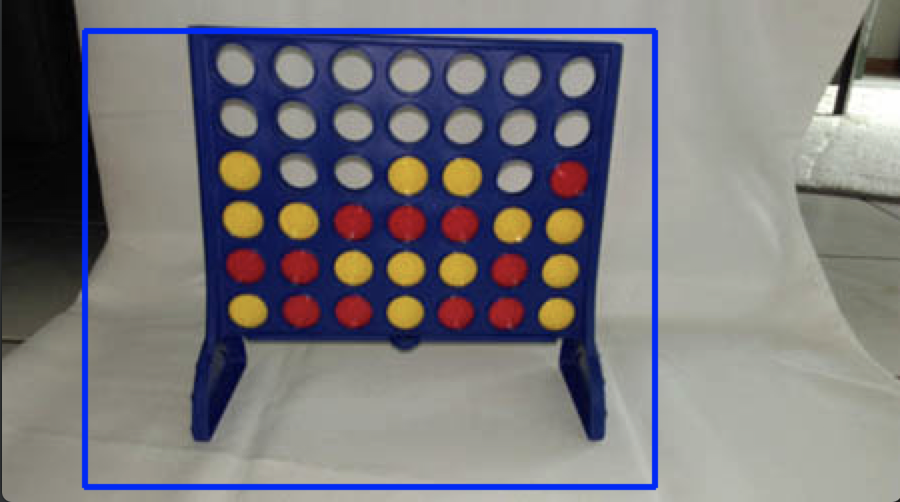
\includegraphics[width = .3\textwidth]{figures/detection.png}
  \caption{Object detection using a Haar Algorithm.}
  \label{fig:haarDetection}
\end{figure}
After several hoursa \textit{cascade.xml} is provided and can be used for image detection easily.

\subsubsection{Filters}
The image undergoes various filter processes for differentiation between yellow, red and blue and background.
At the time this abstract was written, colors are being compared hardcoded, so a couple of references are being provided and then use for comparison.
The image is then divided into multiple binary channels (i.e. red, yellow, blue, background) by a thresholded RGB color comparison.
\begin{figure}[bh]
  \centering
  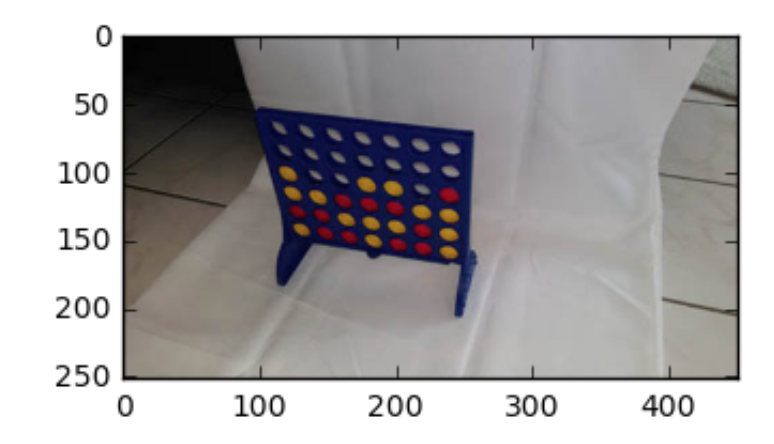
\includegraphics[width = .3\textwidth]{figures/camera.png}
  \caption{Original photograph before image processing.}
  \label{fig:capturedImage}
\end{figure}
\begin{figure}[bh]
  \centering
  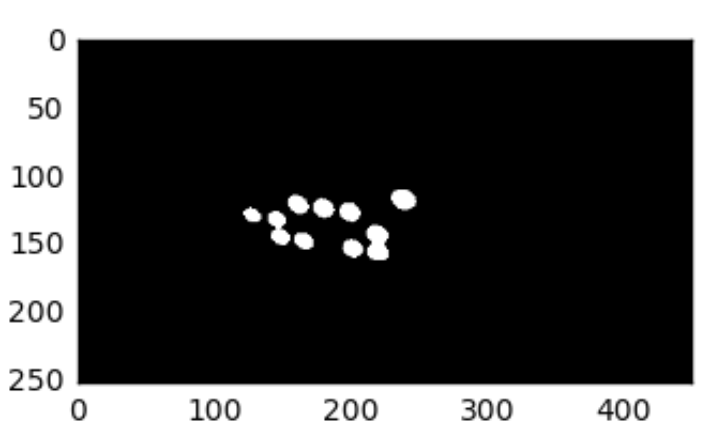
\includegraphics[width = .3\textwidth]{figures/redChannel.png}
  \caption{Extraction of a binary red channel.}
  \label{fig:redChannel}
\end{figure}
\begin{figure}[bh]
  \centering
  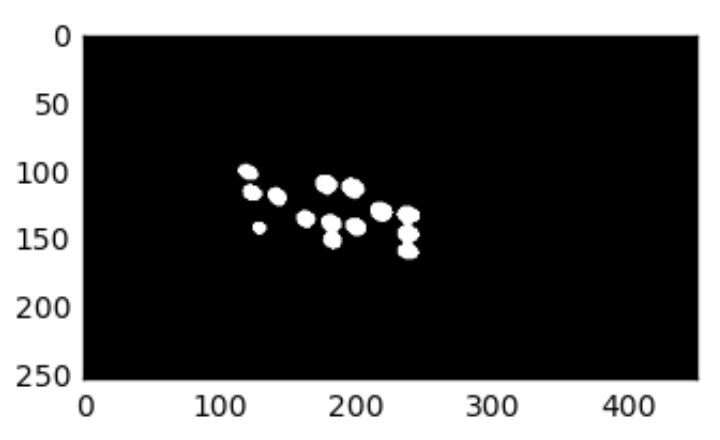
\includegraphics[width = .3\textwidth]{figures/yellowChannel.png}
  \caption{Extraction of a binary yellow channel.}
  \label{fig:yellowChannel}
\end{figure}
% \begin{figure}[bh]
%   \centering
%   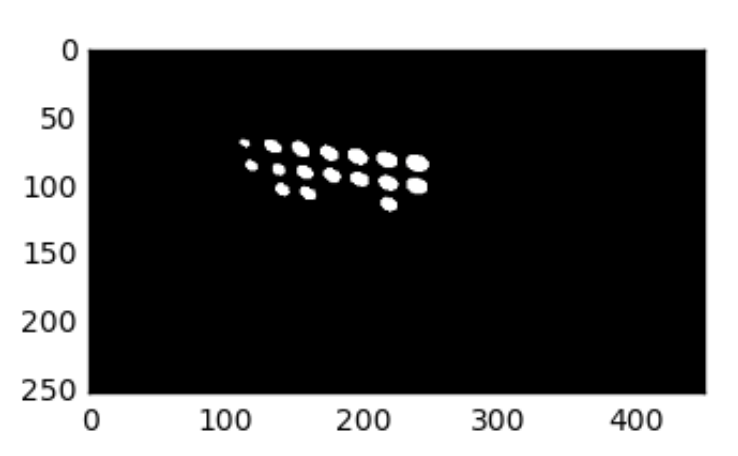
\includegraphics[width = .3\textwidth]{figures/whiteChannel.png}
%   \caption{OExtraction of a binary white channel.}
%   \label{fig:meg}
% \end{figure}
Various steps are done as well, as further optimization of white channels but should not be explained in detail.

\subsection{Transformation}
In the present case, the corners of the connect4 board are needed for the perspective transformation of the board to a standardized one.
All four corners are found by using the brightest pixel of the sum of red, yellow and background channel which is close to a corner.
Using this information, the channels can be retransformed and a regular grid can be applied.
\begin{figure}[bh]
  \centering
  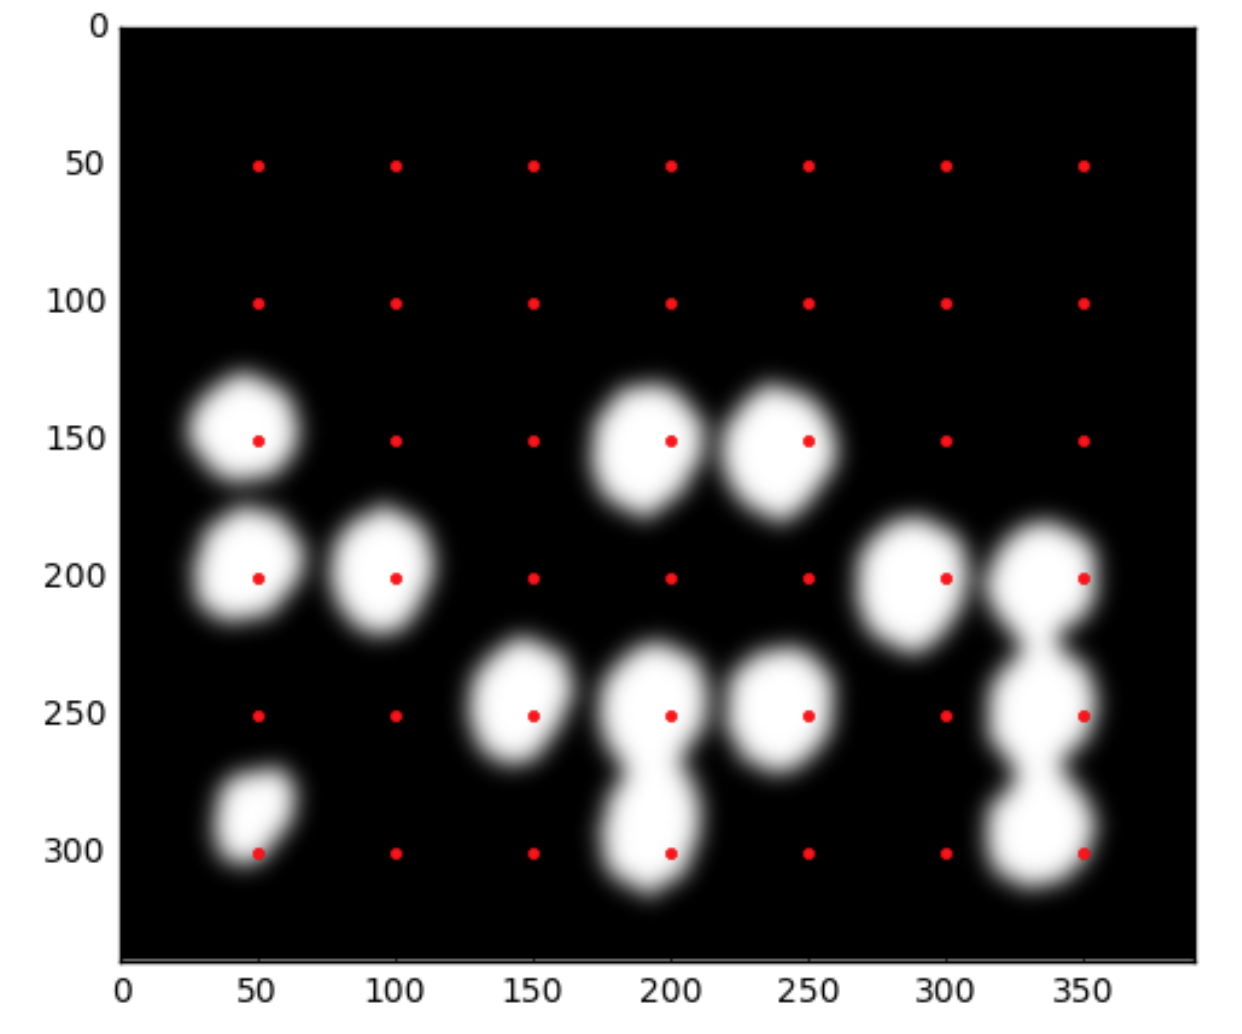
\includegraphics[width = .3\textwidth]{figures/grid.png}
  \caption{Gridpoints of a regular connect4 board.}
  \label{fig:grid}
\end{figure}
\begin{figure}[bh]
  \centering
  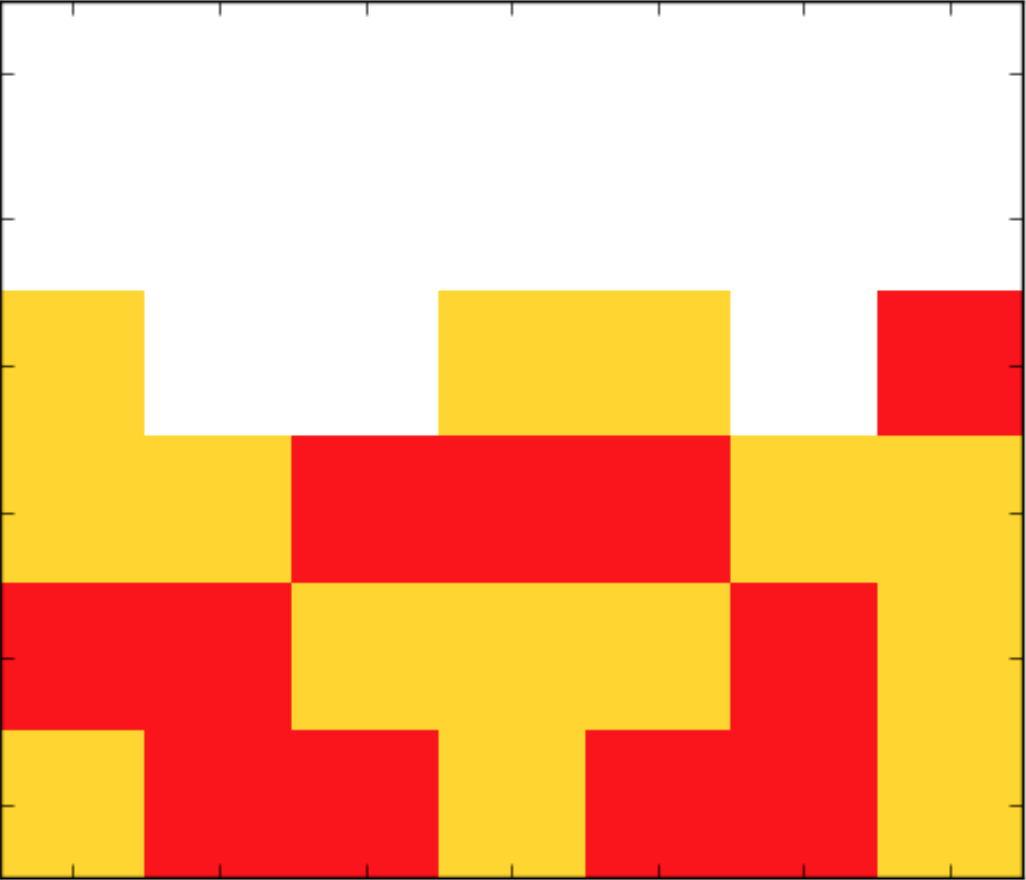
\includegraphics[width = .3\textwidth]{figures/finalBoard.png}
  \caption{Visualisation of final representation of a processed board.}
  \label{fig:final}
\end{figure}


%  by color and pattern comparision.
% The image is then cropped and undergoes various image processing steps, such as wrapping, contrast enhancement and color channel extraction.
% The current board configuration can then be read and converted to a computer readable format by thresholded color comparision.

\subsection{State representation}
Theoretically, we need at least $\lfloor \log_2 3^{6\cdot 7} \rfloor = 67$ bit to store the entire game state, so we could just use a single
128-bit integer to store it.
However, we chose a slightly longer representation by storing the state $s$ in an array of $7$ 16-bit integers $s_i$, one for each column (14 bytes or 112 bit in total).
In each of these integers $s_i$ we assigned two bits for each row of the board, beginning at the lowest two bits with the lowest row.
For every cell, we set the assigned bits to $01$ to represent a coin of player 1, $10$ to represent a coin of player 2 and $00$ to represent an empty cell.

We can now for example efficiently check if a column is full by just checking if the bits of the highest row are set or if the integer value of the column exceeds $0b01000000000$.
Modifying the board and checking for winning positions now just requires some simple bit-wise operations on these integers.

\subsection{Learning}
Our approach to learning the game follows standard reinforcement learning methods.
Our training algorithm performs $N_i$ iterations and simulate $N_g$ games in every iteration.
In each of the simulated games, the moves are determined by a neural network that we will describe in detail below.
The current board state is taken as the input to the neural network and one of the allowed next moves is determined randomly using, weighted by the results of the neural network.
We have only added one single bit of game knowledge to this algorithm: If one of the allowed next moves is a winning move, that move will always be performed.
After the move has ended, a total reward of the end position will be calculated.
We used a reward of $100$ for winning, $-100$ for losing and $-10$ for a draw.

This reward will then be used by the employed algorithms for automatic differentiation and optimization\cite{Adam}, implemented by the software library PyTorch\cite{PyTorch}.

The neural network is constructed of a layer of 42 input neurons, one for each cell of the board, then two layers of 64 neurons each and finally a layer of 8 output neurons, one for each column of the board that the next move could put a coin into.

During the simulations, we experimented with different types of training opponents: random play, random play with winning move recognition and self-play.
In the first case, the opponent just randomly chooses one of the possible moves while in the second case, a random move is chosen except in situations where there is a move that leads to a win of the opponent.
In the third case, the same algorithm and neural network that we train and use for the first player is used for playing both sides (but only the actions of the first player are used for learning).
To avoid the self-play method to just play the same game over and over again, we add some random noise to the decisions of the opponent.

It can be shown that with perfect play on both sides, the first player to insert a coin will always win if and only if they insert their coin in one of the columns adjacent to the middle.
If the first coin is inserted in the outer columns of the game, the second player can win with perfect play.

The consequence of this is that if our learning agent learns the perfect strategy, we would still only see a winning rate of $50\%$ if we randomly
let the agent and its opponent begin.
For simplicity and more understandable results, we therefore assume that our agent always begins the game.

%-------------------------------------------------------------------------
\section{Results}

\subsection{Vision}
The complete image processing time is $< 0.3$ s (i7-4790K CPU @ 4.00GHz) per image.

\subsubsection{Object Detection}
Figure \ref{fig:haarDetection} shows the visulisation of the object detection using Haar wavelet features.
A more simple Local Binary Pattern (LBP) has been tried as well, but lead to fewer succesful detections.

\subsubsection{Filters}
Figure \ref{fig:capturedImage} shows the original image coming from the camera without any image processing steps.
Figure \ref{fig:redChannel} and \ref{fig:yellowChannel} show the binary channels of the board.
Note that all processing steps following object detection are carried out no matter detection was successful or not.
\subsubsection{Transformation}
Figure \ref{fig:grid} shows the perspectively transformed image with gridpoints on top of it.
After this step, the final representation of the board can be seen in \ref{fig:final}.



\subsection{Learning}
Our training algorithm was mainly CPU-bound and using a GPU for tensor
operation did not pose a speed-up since the time wasn't lost in the neural
network computation but in the game logic (e.g. checks for winning position).
We tried to quickly port our Python game logic code to Cython code but were
unable to achieve a speed-up without investing more engineering effort.
In the end, we were able to simulate $N_g = 250$ games and learn from
them within $4\mathrm{s}$ on a fast desktop CPU (i7-4790K @ 4.00 GHz)
or within $8 \mathrm{s}$ on a regular notebook CPU (i5-3210M CPU @ 2.50GHz).

Figure \ref{fig:last_move_self_001} shows the winning rate evolving during
1000 training cycles.
As one can easily see, the winning rate more or less
instantly reaches $70–80 \%$ in self-play and does not really change any more.
Literature suggests that there might be a strong improvement after a huge number of iteration cycles ($> 10^7$) but due to limited project time and server computation resources we haven't been able to research this further.

\begin{figure}[t]
    \begin{center}
		\noindent
		\makebox[3.25in]{
	   		%% Creator: Matplotlib, PGF backend
%%
%% To include the figure in your LaTeX document, write
%%   \input{<filename>.pgf}
%%
%% Make sure the required packages are loaded in your preamble
%%   \usepackage{pgf}
%%
%% Figures using additional raster images can only be included by \input if
%% they are in the same directory as the main LaTeX file. For loading figures
%% from other directories you can use the `import` package
%%   \usepackage{import}
%% and then include the figures with
%%   \import{<path to file>}{<filename>.pgf}
%%
%% Matplotlib used the following preamble
%%   \usepackage{fontspec}
%%   \setmainfont{DejaVu Serif}
%%   \setsansfont{DejaVu Sans}
%%   \setmonofont{DejaVu Sans Mono}
%%
\begingroup%
\makeatletter%
\begin{pgfpicture}%
\pgfpathrectangle{\pgfpointorigin}{\pgfqpoint{3.250000in}{3.000000in}}%
\pgfusepath{use as bounding box, clip}%
\begin{pgfscope}%
\pgfsetbuttcap%
\pgfsetmiterjoin%
\definecolor{currentfill}{rgb}{1.000000,1.000000,1.000000}%
\pgfsetfillcolor{currentfill}%
\pgfsetlinewidth{0.000000pt}%
\definecolor{currentstroke}{rgb}{1.000000,1.000000,1.000000}%
\pgfsetstrokecolor{currentstroke}%
\pgfsetdash{}{0pt}%
\pgfpathmoveto{\pgfqpoint{0.000000in}{0.000000in}}%
\pgfpathlineto{\pgfqpoint{3.250000in}{0.000000in}}%
\pgfpathlineto{\pgfqpoint{3.250000in}{3.000000in}}%
\pgfpathlineto{\pgfqpoint{0.000000in}{3.000000in}}%
\pgfpathclose%
\pgfusepath{fill}%
\end{pgfscope}%
\begin{pgfscope}%
\pgfsetbuttcap%
\pgfsetmiterjoin%
\definecolor{currentfill}{rgb}{1.000000,1.000000,1.000000}%
\pgfsetfillcolor{currentfill}%
\pgfsetlinewidth{0.000000pt}%
\definecolor{currentstroke}{rgb}{0.000000,0.000000,0.000000}%
\pgfsetstrokecolor{currentstroke}%
\pgfsetstrokeopacity{0.000000}%
\pgfsetdash{}{0pt}%
\pgfpathmoveto{\pgfqpoint{0.706528in}{0.582778in}}%
\pgfpathlineto{\pgfqpoint{3.065000in}{0.582778in}}%
\pgfpathlineto{\pgfqpoint{3.065000in}{2.795000in}}%
\pgfpathlineto{\pgfqpoint{0.706528in}{2.795000in}}%
\pgfpathclose%
\pgfusepath{fill}%
\end{pgfscope}%
\begin{pgfscope}%
\pgfsetbuttcap%
\pgfsetroundjoin%
\definecolor{currentfill}{rgb}{0.000000,0.000000,0.000000}%
\pgfsetfillcolor{currentfill}%
\pgfsetlinewidth{0.803000pt}%
\definecolor{currentstroke}{rgb}{0.000000,0.000000,0.000000}%
\pgfsetstrokecolor{currentstroke}%
\pgfsetdash{}{0pt}%
\pgfsys@defobject{currentmarker}{\pgfqpoint{0.000000in}{-0.048611in}}{\pgfqpoint{0.000000in}{0.000000in}}{%
\pgfpathmoveto{\pgfqpoint{0.000000in}{0.000000in}}%
\pgfpathlineto{\pgfqpoint{0.000000in}{-0.048611in}}%
\pgfusepath{stroke,fill}%
}%
\begin{pgfscope}%
\pgfsys@transformshift{0.813731in}{0.582778in}%
\pgfsys@useobject{currentmarker}{}%
\end{pgfscope}%
\end{pgfscope}%
\begin{pgfscope}%
\pgftext[x=0.813731in,y=0.485556in,,top]{\sffamily\fontsize{10.000000}{12.000000}\selectfont 0}%
\end{pgfscope}%
\begin{pgfscope}%
\pgfsetbuttcap%
\pgfsetroundjoin%
\definecolor{currentfill}{rgb}{0.000000,0.000000,0.000000}%
\pgfsetfillcolor{currentfill}%
\pgfsetlinewidth{0.803000pt}%
\definecolor{currentstroke}{rgb}{0.000000,0.000000,0.000000}%
\pgfsetstrokecolor{currentstroke}%
\pgfsetdash{}{0pt}%
\pgfsys@defobject{currentmarker}{\pgfqpoint{0.000000in}{-0.048611in}}{\pgfqpoint{0.000000in}{0.000000in}}{%
\pgfpathmoveto{\pgfqpoint{0.000000in}{0.000000in}}%
\pgfpathlineto{\pgfqpoint{0.000000in}{-0.048611in}}%
\pgfusepath{stroke,fill}%
}%
\begin{pgfscope}%
\pgfsys@transformshift{1.344440in}{0.582778in}%
\pgfsys@useobject{currentmarker}{}%
\end{pgfscope}%
\end{pgfscope}%
\begin{pgfscope}%
\pgftext[x=1.344440in,y=0.485556in,,top]{\sffamily\fontsize{10.000000}{12.000000}\selectfont 25}%
\end{pgfscope}%
\begin{pgfscope}%
\pgfsetbuttcap%
\pgfsetroundjoin%
\definecolor{currentfill}{rgb}{0.000000,0.000000,0.000000}%
\pgfsetfillcolor{currentfill}%
\pgfsetlinewidth{0.803000pt}%
\definecolor{currentstroke}{rgb}{0.000000,0.000000,0.000000}%
\pgfsetstrokecolor{currentstroke}%
\pgfsetdash{}{0pt}%
\pgfsys@defobject{currentmarker}{\pgfqpoint{0.000000in}{-0.048611in}}{\pgfqpoint{0.000000in}{0.000000in}}{%
\pgfpathmoveto{\pgfqpoint{0.000000in}{0.000000in}}%
\pgfpathlineto{\pgfqpoint{0.000000in}{-0.048611in}}%
\pgfusepath{stroke,fill}%
}%
\begin{pgfscope}%
\pgfsys@transformshift{1.875150in}{0.582778in}%
\pgfsys@useobject{currentmarker}{}%
\end{pgfscope}%
\end{pgfscope}%
\begin{pgfscope}%
\pgftext[x=1.875150in,y=0.485556in,,top]{\sffamily\fontsize{10.000000}{12.000000}\selectfont 50}%
\end{pgfscope}%
\begin{pgfscope}%
\pgfsetbuttcap%
\pgfsetroundjoin%
\definecolor{currentfill}{rgb}{0.000000,0.000000,0.000000}%
\pgfsetfillcolor{currentfill}%
\pgfsetlinewidth{0.803000pt}%
\definecolor{currentstroke}{rgb}{0.000000,0.000000,0.000000}%
\pgfsetstrokecolor{currentstroke}%
\pgfsetdash{}{0pt}%
\pgfsys@defobject{currentmarker}{\pgfqpoint{0.000000in}{-0.048611in}}{\pgfqpoint{0.000000in}{0.000000in}}{%
\pgfpathmoveto{\pgfqpoint{0.000000in}{0.000000in}}%
\pgfpathlineto{\pgfqpoint{0.000000in}{-0.048611in}}%
\pgfusepath{stroke,fill}%
}%
\begin{pgfscope}%
\pgfsys@transformshift{2.405859in}{0.582778in}%
\pgfsys@useobject{currentmarker}{}%
\end{pgfscope}%
\end{pgfscope}%
\begin{pgfscope}%
\pgftext[x=2.405859in,y=0.485556in,,top]{\sffamily\fontsize{10.000000}{12.000000}\selectfont 75}%
\end{pgfscope}%
\begin{pgfscope}%
\pgfsetbuttcap%
\pgfsetroundjoin%
\definecolor{currentfill}{rgb}{0.000000,0.000000,0.000000}%
\pgfsetfillcolor{currentfill}%
\pgfsetlinewidth{0.803000pt}%
\definecolor{currentstroke}{rgb}{0.000000,0.000000,0.000000}%
\pgfsetstrokecolor{currentstroke}%
\pgfsetdash{}{0pt}%
\pgfsys@defobject{currentmarker}{\pgfqpoint{0.000000in}{-0.048611in}}{\pgfqpoint{0.000000in}{0.000000in}}{%
\pgfpathmoveto{\pgfqpoint{0.000000in}{0.000000in}}%
\pgfpathlineto{\pgfqpoint{0.000000in}{-0.048611in}}%
\pgfusepath{stroke,fill}%
}%
\begin{pgfscope}%
\pgfsys@transformshift{2.936568in}{0.582778in}%
\pgfsys@useobject{currentmarker}{}%
\end{pgfscope}%
\end{pgfscope}%
\begin{pgfscope}%
\pgftext[x=2.936568in,y=0.485556in,,top]{\sffamily\fontsize{10.000000}{12.000000}\selectfont 100}%
\end{pgfscope}%
\begin{pgfscope}%
\pgftext[x=1.885764in,y=0.295587in,,top]{\sffamily\fontsize{10.000000}{12.000000}\selectfont Iteration}%
\end{pgfscope}%
\begin{pgfscope}%
\pgfsetbuttcap%
\pgfsetroundjoin%
\definecolor{currentfill}{rgb}{0.000000,0.000000,0.000000}%
\pgfsetfillcolor{currentfill}%
\pgfsetlinewidth{0.803000pt}%
\definecolor{currentstroke}{rgb}{0.000000,0.000000,0.000000}%
\pgfsetstrokecolor{currentstroke}%
\pgfsetdash{}{0pt}%
\pgfsys@defobject{currentmarker}{\pgfqpoint{-0.048611in}{0.000000in}}{\pgfqpoint{0.000000in}{0.000000in}}{%
\pgfpathmoveto{\pgfqpoint{0.000000in}{0.000000in}}%
\pgfpathlineto{\pgfqpoint{-0.048611in}{0.000000in}}%
\pgfusepath{stroke,fill}%
}%
\begin{pgfscope}%
\pgfsys@transformshift{0.706528in}{0.582778in}%
\pgfsys@useobject{currentmarker}{}%
\end{pgfscope}%
\end{pgfscope}%
\begin{pgfscope}%
\pgftext[x=0.520940in,y=0.530016in,left,base]{\sffamily\fontsize{10.000000}{12.000000}\selectfont 0}%
\end{pgfscope}%
\begin{pgfscope}%
\pgfsetbuttcap%
\pgfsetroundjoin%
\definecolor{currentfill}{rgb}{0.000000,0.000000,0.000000}%
\pgfsetfillcolor{currentfill}%
\pgfsetlinewidth{0.803000pt}%
\definecolor{currentstroke}{rgb}{0.000000,0.000000,0.000000}%
\pgfsetstrokecolor{currentstroke}%
\pgfsetdash{}{0pt}%
\pgfsys@defobject{currentmarker}{\pgfqpoint{-0.048611in}{0.000000in}}{\pgfqpoint{0.000000in}{0.000000in}}{%
\pgfpathmoveto{\pgfqpoint{0.000000in}{0.000000in}}%
\pgfpathlineto{\pgfqpoint{-0.048611in}{0.000000in}}%
\pgfusepath{stroke,fill}%
}%
\begin{pgfscope}%
\pgfsys@transformshift{0.706528in}{1.025222in}%
\pgfsys@useobject{currentmarker}{}%
\end{pgfscope}%
\end{pgfscope}%
\begin{pgfscope}%
\pgftext[x=0.432575in,y=0.972461in,left,base]{\sffamily\fontsize{10.000000}{12.000000}\selectfont 20}%
\end{pgfscope}%
\begin{pgfscope}%
\pgfsetbuttcap%
\pgfsetroundjoin%
\definecolor{currentfill}{rgb}{0.000000,0.000000,0.000000}%
\pgfsetfillcolor{currentfill}%
\pgfsetlinewidth{0.803000pt}%
\definecolor{currentstroke}{rgb}{0.000000,0.000000,0.000000}%
\pgfsetstrokecolor{currentstroke}%
\pgfsetdash{}{0pt}%
\pgfsys@defobject{currentmarker}{\pgfqpoint{-0.048611in}{0.000000in}}{\pgfqpoint{0.000000in}{0.000000in}}{%
\pgfpathmoveto{\pgfqpoint{0.000000in}{0.000000in}}%
\pgfpathlineto{\pgfqpoint{-0.048611in}{0.000000in}}%
\pgfusepath{stroke,fill}%
}%
\begin{pgfscope}%
\pgfsys@transformshift{0.706528in}{1.467667in}%
\pgfsys@useobject{currentmarker}{}%
\end{pgfscope}%
\end{pgfscope}%
\begin{pgfscope}%
\pgftext[x=0.432575in,y=1.414905in,left,base]{\sffamily\fontsize{10.000000}{12.000000}\selectfont 40}%
\end{pgfscope}%
\begin{pgfscope}%
\pgfsetbuttcap%
\pgfsetroundjoin%
\definecolor{currentfill}{rgb}{0.000000,0.000000,0.000000}%
\pgfsetfillcolor{currentfill}%
\pgfsetlinewidth{0.803000pt}%
\definecolor{currentstroke}{rgb}{0.000000,0.000000,0.000000}%
\pgfsetstrokecolor{currentstroke}%
\pgfsetdash{}{0pt}%
\pgfsys@defobject{currentmarker}{\pgfqpoint{-0.048611in}{0.000000in}}{\pgfqpoint{0.000000in}{0.000000in}}{%
\pgfpathmoveto{\pgfqpoint{0.000000in}{0.000000in}}%
\pgfpathlineto{\pgfqpoint{-0.048611in}{0.000000in}}%
\pgfusepath{stroke,fill}%
}%
\begin{pgfscope}%
\pgfsys@transformshift{0.706528in}{1.910111in}%
\pgfsys@useobject{currentmarker}{}%
\end{pgfscope}%
\end{pgfscope}%
\begin{pgfscope}%
\pgftext[x=0.432575in,y=1.857350in,left,base]{\sffamily\fontsize{10.000000}{12.000000}\selectfont 60}%
\end{pgfscope}%
\begin{pgfscope}%
\pgfsetbuttcap%
\pgfsetroundjoin%
\definecolor{currentfill}{rgb}{0.000000,0.000000,0.000000}%
\pgfsetfillcolor{currentfill}%
\pgfsetlinewidth{0.803000pt}%
\definecolor{currentstroke}{rgb}{0.000000,0.000000,0.000000}%
\pgfsetstrokecolor{currentstroke}%
\pgfsetdash{}{0pt}%
\pgfsys@defobject{currentmarker}{\pgfqpoint{-0.048611in}{0.000000in}}{\pgfqpoint{0.000000in}{0.000000in}}{%
\pgfpathmoveto{\pgfqpoint{0.000000in}{0.000000in}}%
\pgfpathlineto{\pgfqpoint{-0.048611in}{0.000000in}}%
\pgfusepath{stroke,fill}%
}%
\begin{pgfscope}%
\pgfsys@transformshift{0.706528in}{2.352556in}%
\pgfsys@useobject{currentmarker}{}%
\end{pgfscope}%
\end{pgfscope}%
\begin{pgfscope}%
\pgftext[x=0.432575in,y=2.299794in,left,base]{\sffamily\fontsize{10.000000}{12.000000}\selectfont 80}%
\end{pgfscope}%
\begin{pgfscope}%
\pgfsetbuttcap%
\pgfsetroundjoin%
\definecolor{currentfill}{rgb}{0.000000,0.000000,0.000000}%
\pgfsetfillcolor{currentfill}%
\pgfsetlinewidth{0.803000pt}%
\definecolor{currentstroke}{rgb}{0.000000,0.000000,0.000000}%
\pgfsetstrokecolor{currentstroke}%
\pgfsetdash{}{0pt}%
\pgfsys@defobject{currentmarker}{\pgfqpoint{-0.048611in}{0.000000in}}{\pgfqpoint{0.000000in}{0.000000in}}{%
\pgfpathmoveto{\pgfqpoint{0.000000in}{0.000000in}}%
\pgfpathlineto{\pgfqpoint{-0.048611in}{0.000000in}}%
\pgfusepath{stroke,fill}%
}%
\begin{pgfscope}%
\pgfsys@transformshift{0.706528in}{2.795000in}%
\pgfsys@useobject{currentmarker}{}%
\end{pgfscope}%
\end{pgfscope}%
\begin{pgfscope}%
\pgftext[x=0.344210in,y=2.742238in,left,base]{\sffamily\fontsize{10.000000}{12.000000}\selectfont 100}%
\end{pgfscope}%
\begin{pgfscope}%
\pgftext[x=0.288654in,y=1.688889in,,bottom,rotate=90.000000]{\sffamily\fontsize{10.000000}{12.000000}\selectfont Winning rate (\%)}%
\end{pgfscope}%
\begin{pgfscope}%
\pgfpathrectangle{\pgfqpoint{0.706528in}{0.582778in}}{\pgfqpoint{2.358472in}{2.212222in}} %
\pgfusepath{clip}%
\pgfsetrectcap%
\pgfsetroundjoin%
\pgfsetlinewidth{1.505625pt}%
\definecolor{currentstroke}{rgb}{0.121569,0.466667,0.705882}%
\pgfsetstrokecolor{currentstroke}%
\pgfsetdash{}{0pt}%
\pgfpathmoveto{\pgfqpoint{0.813731in}{1.910111in}}%
\pgfpathlineto{\pgfqpoint{0.834959in}{2.060542in}}%
\pgfpathlineto{\pgfqpoint{0.856188in}{2.051693in}}%
\pgfpathlineto{\pgfqpoint{0.877416in}{1.989751in}}%
\pgfpathlineto{\pgfqpoint{0.898645in}{2.087089in}}%
\pgfpathlineto{\pgfqpoint{0.919873in}{2.122484in}}%
\pgfpathlineto{\pgfqpoint{0.941101in}{2.069391in}}%
\pgfpathlineto{\pgfqpoint{0.962330in}{1.980902in}}%
\pgfpathlineto{\pgfqpoint{0.983558in}{2.051693in}}%
\pgfpathlineto{\pgfqpoint{1.004786in}{1.945507in}}%
\pgfpathlineto{\pgfqpoint{1.026015in}{2.033996in}}%
\pgfpathlineto{\pgfqpoint{1.047243in}{2.051693in}}%
\pgfpathlineto{\pgfqpoint{1.068472in}{2.042844in}}%
\pgfpathlineto{\pgfqpoint{1.089700in}{1.901262in}}%
\pgfpathlineto{\pgfqpoint{1.110928in}{1.662342in}}%
\pgfpathlineto{\pgfqpoint{1.132157in}{1.839320in}}%
\pgfpathlineto{\pgfqpoint{1.153385in}{2.033996in}}%
\pgfpathlineto{\pgfqpoint{1.174613in}{1.565004in}}%
\pgfpathlineto{\pgfqpoint{1.195842in}{1.388027in}}%
\pgfpathlineto{\pgfqpoint{1.217070in}{1.467667in}}%
\pgfpathlineto{\pgfqpoint{1.238299in}{2.122484in}}%
\pgfpathlineto{\pgfqpoint{1.259527in}{1.963204in}}%
\pgfpathlineto{\pgfqpoint{1.280755in}{1.874716in}}%
\pgfpathlineto{\pgfqpoint{1.301984in}{2.069391in}}%
\pgfpathlineto{\pgfqpoint{1.323212in}{2.016298in}}%
\pgfpathlineto{\pgfqpoint{1.344440in}{1.963204in}}%
\pgfpathlineto{\pgfqpoint{1.365669in}{1.927809in}}%
\pgfpathlineto{\pgfqpoint{1.386897in}{1.989751in}}%
\pgfpathlineto{\pgfqpoint{1.408126in}{1.927809in}}%
\pgfpathlineto{\pgfqpoint{1.429354in}{1.901262in}}%
\pgfpathlineto{\pgfqpoint{1.450582in}{1.343782in}}%
\pgfpathlineto{\pgfqpoint{1.471811in}{1.458818in}}%
\pgfpathlineto{\pgfqpoint{1.493039in}{1.963204in}}%
\pgfpathlineto{\pgfqpoint{1.514267in}{1.963204in}}%
\pgfpathlineto{\pgfqpoint{1.535496in}{2.087089in}}%
\pgfpathlineto{\pgfqpoint{1.556724in}{1.883564in}}%
\pgfpathlineto{\pgfqpoint{1.577952in}{1.989751in}}%
\pgfpathlineto{\pgfqpoint{1.599181in}{1.963204in}}%
\pgfpathlineto{\pgfqpoint{1.620409in}{2.042844in}}%
\pgfpathlineto{\pgfqpoint{1.641638in}{1.901262in}}%
\pgfpathlineto{\pgfqpoint{1.662866in}{1.954356in}}%
\pgfpathlineto{\pgfqpoint{1.684094in}{2.025147in}}%
\pgfpathlineto{\pgfqpoint{1.705323in}{1.989751in}}%
\pgfpathlineto{\pgfqpoint{1.726551in}{2.025147in}}%
\pgfpathlineto{\pgfqpoint{1.747779in}{1.963204in}}%
\pgfpathlineto{\pgfqpoint{1.769008in}{2.025147in}}%
\pgfpathlineto{\pgfqpoint{1.790236in}{2.007449in}}%
\pgfpathlineto{\pgfqpoint{1.811465in}{2.007449in}}%
\pgfpathlineto{\pgfqpoint{1.832693in}{2.025147in}}%
\pgfpathlineto{\pgfqpoint{1.853921in}{1.963204in}}%
\pgfpathlineto{\pgfqpoint{1.875150in}{2.033996in}}%
\pgfpathlineto{\pgfqpoint{1.896378in}{2.122484in}}%
\pgfpathlineto{\pgfqpoint{1.917606in}{1.848169in}}%
\pgfpathlineto{\pgfqpoint{1.938835in}{1.927809in}}%
\pgfpathlineto{\pgfqpoint{1.960063in}{1.954356in}}%
\pgfpathlineto{\pgfqpoint{1.981292in}{1.927809in}}%
\pgfpathlineto{\pgfqpoint{2.002520in}{1.892413in}}%
\pgfpathlineto{\pgfqpoint{2.023748in}{1.927809in}}%
\pgfpathlineto{\pgfqpoint{2.044977in}{1.901262in}}%
\pgfpathlineto{\pgfqpoint{2.066205in}{2.016298in}}%
\pgfpathlineto{\pgfqpoint{2.087433in}{1.803924in}}%
\pgfpathlineto{\pgfqpoint{2.108662in}{2.042844in}}%
\pgfpathlineto{\pgfqpoint{2.129890in}{1.980902in}}%
\pgfpathlineto{\pgfqpoint{2.151119in}{1.945507in}}%
\pgfpathlineto{\pgfqpoint{2.172347in}{2.060542in}}%
\pgfpathlineto{\pgfqpoint{2.193575in}{2.007449in}}%
\pgfpathlineto{\pgfqpoint{2.214804in}{1.954356in}}%
\pgfpathlineto{\pgfqpoint{2.236032in}{1.963204in}}%
\pgfpathlineto{\pgfqpoint{2.257260in}{1.936658in}}%
\pgfpathlineto{\pgfqpoint{2.278489in}{1.892413in}}%
\pgfpathlineto{\pgfqpoint{2.299717in}{2.060542in}}%
\pgfpathlineto{\pgfqpoint{2.320946in}{1.972053in}}%
\pgfpathlineto{\pgfqpoint{2.342174in}{1.892413in}}%
\pgfpathlineto{\pgfqpoint{2.363402in}{2.033996in}}%
\pgfpathlineto{\pgfqpoint{2.384631in}{1.812773in}}%
\pgfpathlineto{\pgfqpoint{2.405859in}{1.980902in}}%
\pgfpathlineto{\pgfqpoint{2.427087in}{1.865867in}}%
\pgfpathlineto{\pgfqpoint{2.448316in}{2.007449in}}%
\pgfpathlineto{\pgfqpoint{2.469544in}{2.051693in}}%
\pgfpathlineto{\pgfqpoint{2.490773in}{1.963204in}}%
\pgfpathlineto{\pgfqpoint{2.512001in}{2.007449in}}%
\pgfpathlineto{\pgfqpoint{2.533229in}{1.759680in}}%
\pgfpathlineto{\pgfqpoint{2.554458in}{2.087089in}}%
\pgfpathlineto{\pgfqpoint{2.575686in}{1.857018in}}%
\pgfpathlineto{\pgfqpoint{2.596914in}{1.936658in}}%
\pgfpathlineto{\pgfqpoint{2.618143in}{1.927809in}}%
\pgfpathlineto{\pgfqpoint{2.639371in}{1.998600in}}%
\pgfpathlineto{\pgfqpoint{2.660599in}{2.033996in}}%
\pgfpathlineto{\pgfqpoint{2.681828in}{1.892413in}}%
\pgfpathlineto{\pgfqpoint{2.703056in}{1.963204in}}%
\pgfpathlineto{\pgfqpoint{2.724285in}{2.069391in}}%
\pgfpathlineto{\pgfqpoint{2.745513in}{1.927809in}}%
\pgfpathlineto{\pgfqpoint{2.766741in}{1.927809in}}%
\pgfpathlineto{\pgfqpoint{2.787970in}{1.989751in}}%
\pgfpathlineto{\pgfqpoint{2.809198in}{1.927809in}}%
\pgfpathlineto{\pgfqpoint{2.830426in}{1.963204in}}%
\pgfpathlineto{\pgfqpoint{2.851655in}{1.972053in}}%
\pgfpathlineto{\pgfqpoint{2.872883in}{1.812773in}}%
\pgfpathlineto{\pgfqpoint{2.894112in}{1.972053in}}%
\pgfpathlineto{\pgfqpoint{2.915340in}{1.989751in}}%
\pgfpathlineto{\pgfqpoint{2.936568in}{1.954356in}}%
\pgfpathlineto{\pgfqpoint{2.957797in}{1.857018in}}%
\pgfusepath{stroke}%
\end{pgfscope}%
\begin{pgfscope}%
\pgfsetrectcap%
\pgfsetmiterjoin%
\pgfsetlinewidth{0.803000pt}%
\definecolor{currentstroke}{rgb}{0.000000,0.000000,0.000000}%
\pgfsetstrokecolor{currentstroke}%
\pgfsetdash{}{0pt}%
\pgfpathmoveto{\pgfqpoint{0.706528in}{0.582778in}}%
\pgfpathlineto{\pgfqpoint{0.706528in}{2.795000in}}%
\pgfusepath{stroke}%
\end{pgfscope}%
\begin{pgfscope}%
\pgfsetrectcap%
\pgfsetmiterjoin%
\pgfsetlinewidth{0.803000pt}%
\definecolor{currentstroke}{rgb}{0.000000,0.000000,0.000000}%
\pgfsetstrokecolor{currentstroke}%
\pgfsetdash{}{0pt}%
\pgfpathmoveto{\pgfqpoint{3.065000in}{0.582778in}}%
\pgfpathlineto{\pgfqpoint{3.065000in}{2.795000in}}%
\pgfusepath{stroke}%
\end{pgfscope}%
\begin{pgfscope}%
\pgfsetrectcap%
\pgfsetmiterjoin%
\pgfsetlinewidth{0.803000pt}%
\definecolor{currentstroke}{rgb}{0.000000,0.000000,0.000000}%
\pgfsetstrokecolor{currentstroke}%
\pgfsetdash{}{0pt}%
\pgfpathmoveto{\pgfqpoint{0.706528in}{0.582778in}}%
\pgfpathlineto{\pgfqpoint{3.065000in}{0.582778in}}%
\pgfusepath{stroke}%
\end{pgfscope}%
\begin{pgfscope}%
\pgfsetrectcap%
\pgfsetmiterjoin%
\pgfsetlinewidth{0.803000pt}%
\definecolor{currentstroke}{rgb}{0.000000,0.000000,0.000000}%
\pgfsetstrokecolor{currentstroke}%
\pgfsetdash{}{0pt}%
\pgfpathmoveto{\pgfqpoint{0.706528in}{2.795000in}}%
\pgfpathlineto{\pgfqpoint{3.065000in}{2.795000in}}%
\pgfusepath{stroke}%
\end{pgfscope}%
\end{pgfpicture}%
\makeatother%
\endgroup%

		}
	\end{center}
    \caption{Training with $N_g=250$, self play with $1\%$ noise, reward given for last move.}
	\label{fig:last_move_self_001}
\end{figure}
We tested different ways to propagate the reward used for the reinforcement learning algorithm.
In most cases, we just assigned the total reward $r_{total}$ to the last move of the game and did not explicitly specify a reward for all other moves.
In one experiment, we instead set the reward
As Figure \ref{fig:all_moves_self_001} shows, this change does not visibly change the results.
\begin{figure}[t]
    \begin{center}
		\noindent
		\makebox[3.25in]{
	   		%% Creator: Matplotlib, PGF backend
%%
%% To include the figure in your LaTeX document, write
%%   \input{<filename>.pgf}
%%
%% Make sure the required packages are loaded in your preamble
%%   \usepackage{pgf}
%%
%% Figures using additional raster images can only be included by \input if
%% they are in the same directory as the main LaTeX file. For loading figures
%% from other directories you can use the `import` package
%%   \usepackage{import}
%% and then include the figures with
%%   \import{<path to file>}{<filename>.pgf}
%%
%% Matplotlib used the following preamble
%%   \usepackage{fontspec}
%%   \setmainfont{DejaVu Serif}
%%   \setsansfont{DejaVu Sans}
%%   \setmonofont{DejaVu Sans Mono}
%%
\begingroup%
\makeatletter%
\begin{pgfpicture}%
\pgfpathrectangle{\pgfpointorigin}{\pgfqpoint{3.250000in}{3.000000in}}%
\pgfusepath{use as bounding box, clip}%
\begin{pgfscope}%
\pgfsetbuttcap%
\pgfsetmiterjoin%
\definecolor{currentfill}{rgb}{1.000000,1.000000,1.000000}%
\pgfsetfillcolor{currentfill}%
\pgfsetlinewidth{0.000000pt}%
\definecolor{currentstroke}{rgb}{1.000000,1.000000,1.000000}%
\pgfsetstrokecolor{currentstroke}%
\pgfsetdash{}{0pt}%
\pgfpathmoveto{\pgfqpoint{0.000000in}{0.000000in}}%
\pgfpathlineto{\pgfqpoint{3.250000in}{0.000000in}}%
\pgfpathlineto{\pgfqpoint{3.250000in}{3.000000in}}%
\pgfpathlineto{\pgfqpoint{0.000000in}{3.000000in}}%
\pgfpathclose%
\pgfusepath{fill}%
\end{pgfscope}%
\begin{pgfscope}%
\pgfsetbuttcap%
\pgfsetmiterjoin%
\definecolor{currentfill}{rgb}{1.000000,1.000000,1.000000}%
\pgfsetfillcolor{currentfill}%
\pgfsetlinewidth{0.000000pt}%
\definecolor{currentstroke}{rgb}{0.000000,0.000000,0.000000}%
\pgfsetstrokecolor{currentstroke}%
\pgfsetstrokeopacity{0.000000}%
\pgfsetdash{}{0pt}%
\pgfpathmoveto{\pgfqpoint{0.706528in}{0.582778in}}%
\pgfpathlineto{\pgfqpoint{3.036572in}{0.582778in}}%
\pgfpathlineto{\pgfqpoint{3.036572in}{2.795000in}}%
\pgfpathlineto{\pgfqpoint{0.706528in}{2.795000in}}%
\pgfpathclose%
\pgfusepath{fill}%
\end{pgfscope}%
\begin{pgfscope}%
\pgfsetbuttcap%
\pgfsetroundjoin%
\definecolor{currentfill}{rgb}{0.000000,0.000000,0.000000}%
\pgfsetfillcolor{currentfill}%
\pgfsetlinewidth{0.803000pt}%
\definecolor{currentstroke}{rgb}{0.000000,0.000000,0.000000}%
\pgfsetstrokecolor{currentstroke}%
\pgfsetdash{}{0pt}%
\pgfsys@defobject{currentmarker}{\pgfqpoint{0.000000in}{-0.048611in}}{\pgfqpoint{0.000000in}{0.000000in}}{%
\pgfpathmoveto{\pgfqpoint{0.000000in}{0.000000in}}%
\pgfpathlineto{\pgfqpoint{0.000000in}{-0.048611in}}%
\pgfusepath{stroke,fill}%
}%
\begin{pgfscope}%
\pgfsys@transformshift{0.812439in}{0.582778in}%
\pgfsys@useobject{currentmarker}{}%
\end{pgfscope}%
\end{pgfscope}%
\begin{pgfscope}%
\pgftext[x=0.812439in,y=0.485556in,,top]{\sffamily\fontsize{10.000000}{12.000000}\selectfont 0}%
\end{pgfscope}%
\begin{pgfscope}%
\pgfsetbuttcap%
\pgfsetroundjoin%
\definecolor{currentfill}{rgb}{0.000000,0.000000,0.000000}%
\pgfsetfillcolor{currentfill}%
\pgfsetlinewidth{0.803000pt}%
\definecolor{currentstroke}{rgb}{0.000000,0.000000,0.000000}%
\pgfsetstrokecolor{currentstroke}%
\pgfsetdash{}{0pt}%
\pgfsys@defobject{currentmarker}{\pgfqpoint{0.000000in}{-0.048611in}}{\pgfqpoint{0.000000in}{0.000000in}}{%
\pgfpathmoveto{\pgfqpoint{0.000000in}{0.000000in}}%
\pgfpathlineto{\pgfqpoint{0.000000in}{-0.048611in}}%
\pgfusepath{stroke,fill}%
}%
\begin{pgfscope}%
\pgfsys@transformshift{1.342524in}{0.582778in}%
\pgfsys@useobject{currentmarker}{}%
\end{pgfscope}%
\end{pgfscope}%
\begin{pgfscope}%
\pgftext[x=1.342524in,y=0.485556in,,top]{\sffamily\fontsize{10.000000}{12.000000}\selectfont 250}%
\end{pgfscope}%
\begin{pgfscope}%
\pgfsetbuttcap%
\pgfsetroundjoin%
\definecolor{currentfill}{rgb}{0.000000,0.000000,0.000000}%
\pgfsetfillcolor{currentfill}%
\pgfsetlinewidth{0.803000pt}%
\definecolor{currentstroke}{rgb}{0.000000,0.000000,0.000000}%
\pgfsetstrokecolor{currentstroke}%
\pgfsetdash{}{0pt}%
\pgfsys@defobject{currentmarker}{\pgfqpoint{0.000000in}{-0.048611in}}{\pgfqpoint{0.000000in}{0.000000in}}{%
\pgfpathmoveto{\pgfqpoint{0.000000in}{0.000000in}}%
\pgfpathlineto{\pgfqpoint{0.000000in}{-0.048611in}}%
\pgfusepath{stroke,fill}%
}%
\begin{pgfscope}%
\pgfsys@transformshift{1.872610in}{0.582778in}%
\pgfsys@useobject{currentmarker}{}%
\end{pgfscope}%
\end{pgfscope}%
\begin{pgfscope}%
\pgftext[x=1.872610in,y=0.485556in,,top]{\sffamily\fontsize{10.000000}{12.000000}\selectfont 500}%
\end{pgfscope}%
\begin{pgfscope}%
\pgfsetbuttcap%
\pgfsetroundjoin%
\definecolor{currentfill}{rgb}{0.000000,0.000000,0.000000}%
\pgfsetfillcolor{currentfill}%
\pgfsetlinewidth{0.803000pt}%
\definecolor{currentstroke}{rgb}{0.000000,0.000000,0.000000}%
\pgfsetstrokecolor{currentstroke}%
\pgfsetdash{}{0pt}%
\pgfsys@defobject{currentmarker}{\pgfqpoint{0.000000in}{-0.048611in}}{\pgfqpoint{0.000000in}{0.000000in}}{%
\pgfpathmoveto{\pgfqpoint{0.000000in}{0.000000in}}%
\pgfpathlineto{\pgfqpoint{0.000000in}{-0.048611in}}%
\pgfusepath{stroke,fill}%
}%
\begin{pgfscope}%
\pgfsys@transformshift{2.402695in}{0.582778in}%
\pgfsys@useobject{currentmarker}{}%
\end{pgfscope}%
\end{pgfscope}%
\begin{pgfscope}%
\pgftext[x=2.402695in,y=0.485556in,,top]{\sffamily\fontsize{10.000000}{12.000000}\selectfont 750}%
\end{pgfscope}%
\begin{pgfscope}%
\pgfsetbuttcap%
\pgfsetroundjoin%
\definecolor{currentfill}{rgb}{0.000000,0.000000,0.000000}%
\pgfsetfillcolor{currentfill}%
\pgfsetlinewidth{0.803000pt}%
\definecolor{currentstroke}{rgb}{0.000000,0.000000,0.000000}%
\pgfsetstrokecolor{currentstroke}%
\pgfsetdash{}{0pt}%
\pgfsys@defobject{currentmarker}{\pgfqpoint{0.000000in}{-0.048611in}}{\pgfqpoint{0.000000in}{0.000000in}}{%
\pgfpathmoveto{\pgfqpoint{0.000000in}{0.000000in}}%
\pgfpathlineto{\pgfqpoint{0.000000in}{-0.048611in}}%
\pgfusepath{stroke,fill}%
}%
\begin{pgfscope}%
\pgfsys@transformshift{2.932781in}{0.582778in}%
\pgfsys@useobject{currentmarker}{}%
\end{pgfscope}%
\end{pgfscope}%
\begin{pgfscope}%
\pgftext[x=2.932781in,y=0.485556in,,top]{\sffamily\fontsize{10.000000}{12.000000}\selectfont 1000}%
\end{pgfscope}%
\begin{pgfscope}%
\pgftext[x=1.871550in,y=0.295587in,,top]{\sffamily\fontsize{10.000000}{12.000000}\selectfont Iteration}%
\end{pgfscope}%
\begin{pgfscope}%
\pgfsetbuttcap%
\pgfsetroundjoin%
\definecolor{currentfill}{rgb}{0.000000,0.000000,0.000000}%
\pgfsetfillcolor{currentfill}%
\pgfsetlinewidth{0.803000pt}%
\definecolor{currentstroke}{rgb}{0.000000,0.000000,0.000000}%
\pgfsetstrokecolor{currentstroke}%
\pgfsetdash{}{0pt}%
\pgfsys@defobject{currentmarker}{\pgfqpoint{-0.048611in}{0.000000in}}{\pgfqpoint{0.000000in}{0.000000in}}{%
\pgfpathmoveto{\pgfqpoint{0.000000in}{0.000000in}}%
\pgfpathlineto{\pgfqpoint{-0.048611in}{0.000000in}}%
\pgfusepath{stroke,fill}%
}%
\begin{pgfscope}%
\pgfsys@transformshift{0.706528in}{0.582778in}%
\pgfsys@useobject{currentmarker}{}%
\end{pgfscope}%
\end{pgfscope}%
\begin{pgfscope}%
\pgftext[x=0.520940in,y=0.530016in,left,base]{\sffamily\fontsize{10.000000}{12.000000}\selectfont 0}%
\end{pgfscope}%
\begin{pgfscope}%
\pgfsetbuttcap%
\pgfsetroundjoin%
\definecolor{currentfill}{rgb}{0.000000,0.000000,0.000000}%
\pgfsetfillcolor{currentfill}%
\pgfsetlinewidth{0.803000pt}%
\definecolor{currentstroke}{rgb}{0.000000,0.000000,0.000000}%
\pgfsetstrokecolor{currentstroke}%
\pgfsetdash{}{0pt}%
\pgfsys@defobject{currentmarker}{\pgfqpoint{-0.048611in}{0.000000in}}{\pgfqpoint{0.000000in}{0.000000in}}{%
\pgfpathmoveto{\pgfqpoint{0.000000in}{0.000000in}}%
\pgfpathlineto{\pgfqpoint{-0.048611in}{0.000000in}}%
\pgfusepath{stroke,fill}%
}%
\begin{pgfscope}%
\pgfsys@transformshift{0.706528in}{1.025222in}%
\pgfsys@useobject{currentmarker}{}%
\end{pgfscope}%
\end{pgfscope}%
\begin{pgfscope}%
\pgftext[x=0.432575in,y=0.972461in,left,base]{\sffamily\fontsize{10.000000}{12.000000}\selectfont 20}%
\end{pgfscope}%
\begin{pgfscope}%
\pgfsetbuttcap%
\pgfsetroundjoin%
\definecolor{currentfill}{rgb}{0.000000,0.000000,0.000000}%
\pgfsetfillcolor{currentfill}%
\pgfsetlinewidth{0.803000pt}%
\definecolor{currentstroke}{rgb}{0.000000,0.000000,0.000000}%
\pgfsetstrokecolor{currentstroke}%
\pgfsetdash{}{0pt}%
\pgfsys@defobject{currentmarker}{\pgfqpoint{-0.048611in}{0.000000in}}{\pgfqpoint{0.000000in}{0.000000in}}{%
\pgfpathmoveto{\pgfqpoint{0.000000in}{0.000000in}}%
\pgfpathlineto{\pgfqpoint{-0.048611in}{0.000000in}}%
\pgfusepath{stroke,fill}%
}%
\begin{pgfscope}%
\pgfsys@transformshift{0.706528in}{1.467667in}%
\pgfsys@useobject{currentmarker}{}%
\end{pgfscope}%
\end{pgfscope}%
\begin{pgfscope}%
\pgftext[x=0.432575in,y=1.414905in,left,base]{\sffamily\fontsize{10.000000}{12.000000}\selectfont 40}%
\end{pgfscope}%
\begin{pgfscope}%
\pgfsetbuttcap%
\pgfsetroundjoin%
\definecolor{currentfill}{rgb}{0.000000,0.000000,0.000000}%
\pgfsetfillcolor{currentfill}%
\pgfsetlinewidth{0.803000pt}%
\definecolor{currentstroke}{rgb}{0.000000,0.000000,0.000000}%
\pgfsetstrokecolor{currentstroke}%
\pgfsetdash{}{0pt}%
\pgfsys@defobject{currentmarker}{\pgfqpoint{-0.048611in}{0.000000in}}{\pgfqpoint{0.000000in}{0.000000in}}{%
\pgfpathmoveto{\pgfqpoint{0.000000in}{0.000000in}}%
\pgfpathlineto{\pgfqpoint{-0.048611in}{0.000000in}}%
\pgfusepath{stroke,fill}%
}%
\begin{pgfscope}%
\pgfsys@transformshift{0.706528in}{1.910111in}%
\pgfsys@useobject{currentmarker}{}%
\end{pgfscope}%
\end{pgfscope}%
\begin{pgfscope}%
\pgftext[x=0.432575in,y=1.857350in,left,base]{\sffamily\fontsize{10.000000}{12.000000}\selectfont 60}%
\end{pgfscope}%
\begin{pgfscope}%
\pgfsetbuttcap%
\pgfsetroundjoin%
\definecolor{currentfill}{rgb}{0.000000,0.000000,0.000000}%
\pgfsetfillcolor{currentfill}%
\pgfsetlinewidth{0.803000pt}%
\definecolor{currentstroke}{rgb}{0.000000,0.000000,0.000000}%
\pgfsetstrokecolor{currentstroke}%
\pgfsetdash{}{0pt}%
\pgfsys@defobject{currentmarker}{\pgfqpoint{-0.048611in}{0.000000in}}{\pgfqpoint{0.000000in}{0.000000in}}{%
\pgfpathmoveto{\pgfqpoint{0.000000in}{0.000000in}}%
\pgfpathlineto{\pgfqpoint{-0.048611in}{0.000000in}}%
\pgfusepath{stroke,fill}%
}%
\begin{pgfscope}%
\pgfsys@transformshift{0.706528in}{2.352556in}%
\pgfsys@useobject{currentmarker}{}%
\end{pgfscope}%
\end{pgfscope}%
\begin{pgfscope}%
\pgftext[x=0.432575in,y=2.299794in,left,base]{\sffamily\fontsize{10.000000}{12.000000}\selectfont 80}%
\end{pgfscope}%
\begin{pgfscope}%
\pgfsetbuttcap%
\pgfsetroundjoin%
\definecolor{currentfill}{rgb}{0.000000,0.000000,0.000000}%
\pgfsetfillcolor{currentfill}%
\pgfsetlinewidth{0.803000pt}%
\definecolor{currentstroke}{rgb}{0.000000,0.000000,0.000000}%
\pgfsetstrokecolor{currentstroke}%
\pgfsetdash{}{0pt}%
\pgfsys@defobject{currentmarker}{\pgfqpoint{-0.048611in}{0.000000in}}{\pgfqpoint{0.000000in}{0.000000in}}{%
\pgfpathmoveto{\pgfqpoint{0.000000in}{0.000000in}}%
\pgfpathlineto{\pgfqpoint{-0.048611in}{0.000000in}}%
\pgfusepath{stroke,fill}%
}%
\begin{pgfscope}%
\pgfsys@transformshift{0.706528in}{2.795000in}%
\pgfsys@useobject{currentmarker}{}%
\end{pgfscope}%
\end{pgfscope}%
\begin{pgfscope}%
\pgftext[x=0.344210in,y=2.742238in,left,base]{\sffamily\fontsize{10.000000}{12.000000}\selectfont 100}%
\end{pgfscope}%
\begin{pgfscope}%
\pgftext[x=0.288654in,y=1.688889in,,bottom,rotate=90.000000]{\sffamily\fontsize{10.000000}{12.000000}\selectfont Winning rate (\%)}%
\end{pgfscope}%
\begin{pgfscope}%
\pgfpathrectangle{\pgfqpoint{0.706528in}{0.582778in}}{\pgfqpoint{2.330044in}{2.212222in}} %
\pgfusepath{clip}%
\pgfsetrectcap%
\pgfsetroundjoin%
\pgfsetlinewidth{1.505625pt}%
\definecolor{currentstroke}{rgb}{0.121569,0.466667,0.705882}%
\pgfsetstrokecolor{currentstroke}%
\pgfsetdash{}{0pt}%
\pgfpathmoveto{\pgfqpoint{0.812439in}{1.821622in}}%
\pgfpathlineto{\pgfqpoint{0.814559in}{2.193276in}}%
\pgfpathlineto{\pgfqpoint{0.816680in}{2.175578in}}%
\pgfpathlineto{\pgfqpoint{0.820920in}{2.246369in}}%
\pgfpathlineto{\pgfqpoint{0.823041in}{2.175578in}}%
\pgfpathlineto{\pgfqpoint{0.825161in}{2.157880in}}%
\pgfpathlineto{\pgfqpoint{0.827281in}{2.113636in}}%
\pgfpathlineto{\pgfqpoint{0.831522in}{2.255218in}}%
\pgfpathlineto{\pgfqpoint{0.833642in}{2.290613in}}%
\pgfpathlineto{\pgfqpoint{0.835763in}{2.255218in}}%
\pgfpathlineto{\pgfqpoint{0.837883in}{2.228671in}}%
\pgfpathlineto{\pgfqpoint{0.840003in}{2.184427in}}%
\pgfpathlineto{\pgfqpoint{0.842124in}{2.290613in}}%
\pgfpathlineto{\pgfqpoint{0.844244in}{2.193276in}}%
\pgfpathlineto{\pgfqpoint{0.846364in}{2.308311in}}%
\pgfpathlineto{\pgfqpoint{0.848485in}{2.219822in}}%
\pgfpathlineto{\pgfqpoint{0.850605in}{2.113636in}}%
\pgfpathlineto{\pgfqpoint{0.852725in}{2.317160in}}%
\pgfpathlineto{\pgfqpoint{0.856966in}{2.175578in}}%
\pgfpathlineto{\pgfqpoint{0.859086in}{2.202124in}}%
\pgfpathlineto{\pgfqpoint{0.861207in}{2.131333in}}%
\pgfpathlineto{\pgfqpoint{0.863327in}{2.202124in}}%
\pgfpathlineto{\pgfqpoint{0.865447in}{2.202124in}}%
\pgfpathlineto{\pgfqpoint{0.867568in}{2.122484in}}%
\pgfpathlineto{\pgfqpoint{0.869688in}{2.157880in}}%
\pgfpathlineto{\pgfqpoint{0.871808in}{2.246369in}}%
\pgfpathlineto{\pgfqpoint{0.873929in}{2.308311in}}%
\pgfpathlineto{\pgfqpoint{0.876049in}{2.210973in}}%
\pgfpathlineto{\pgfqpoint{0.878169in}{2.095938in}}%
\pgfpathlineto{\pgfqpoint{0.880290in}{2.228671in}}%
\pgfpathlineto{\pgfqpoint{0.882410in}{2.166729in}}%
\pgfpathlineto{\pgfqpoint{0.884530in}{2.140182in}}%
\pgfpathlineto{\pgfqpoint{0.886651in}{2.210973in}}%
\pgfpathlineto{\pgfqpoint{0.888771in}{2.210973in}}%
\pgfpathlineto{\pgfqpoint{0.890892in}{2.069391in}}%
\pgfpathlineto{\pgfqpoint{0.893012in}{2.281764in}}%
\pgfpathlineto{\pgfqpoint{0.895132in}{2.166729in}}%
\pgfpathlineto{\pgfqpoint{0.897253in}{2.202124in}}%
\pgfpathlineto{\pgfqpoint{0.899373in}{2.113636in}}%
\pgfpathlineto{\pgfqpoint{0.901493in}{2.255218in}}%
\pgfpathlineto{\pgfqpoint{0.903614in}{2.166729in}}%
\pgfpathlineto{\pgfqpoint{0.905734in}{2.122484in}}%
\pgfpathlineto{\pgfqpoint{0.907854in}{2.299462in}}%
\pgfpathlineto{\pgfqpoint{0.909975in}{2.157880in}}%
\pgfpathlineto{\pgfqpoint{0.912095in}{2.246369in}}%
\pgfpathlineto{\pgfqpoint{0.914215in}{2.272916in}}%
\pgfpathlineto{\pgfqpoint{0.916336in}{2.228671in}}%
\pgfpathlineto{\pgfqpoint{0.918456in}{1.989751in}}%
\pgfpathlineto{\pgfqpoint{0.920576in}{2.140182in}}%
\pgfpathlineto{\pgfqpoint{0.922697in}{2.122484in}}%
\pgfpathlineto{\pgfqpoint{0.924817in}{2.219822in}}%
\pgfpathlineto{\pgfqpoint{0.926937in}{2.166729in}}%
\pgfpathlineto{\pgfqpoint{0.929058in}{2.149031in}}%
\pgfpathlineto{\pgfqpoint{0.931178in}{2.281764in}}%
\pgfpathlineto{\pgfqpoint{0.933298in}{2.219822in}}%
\pgfpathlineto{\pgfqpoint{0.935419in}{2.193276in}}%
\pgfpathlineto{\pgfqpoint{0.937539in}{2.246369in}}%
\pgfpathlineto{\pgfqpoint{0.939659in}{2.060542in}}%
\pgfpathlineto{\pgfqpoint{0.941780in}{2.281764in}}%
\pgfpathlineto{\pgfqpoint{0.946020in}{2.193276in}}%
\pgfpathlineto{\pgfqpoint{0.948141in}{2.175578in}}%
\pgfpathlineto{\pgfqpoint{0.950261in}{2.246369in}}%
\pgfpathlineto{\pgfqpoint{0.952381in}{2.140182in}}%
\pgfpathlineto{\pgfqpoint{0.954502in}{2.104787in}}%
\pgfpathlineto{\pgfqpoint{0.956622in}{2.281764in}}%
\pgfpathlineto{\pgfqpoint{0.958742in}{2.210973in}}%
\pgfpathlineto{\pgfqpoint{0.960863in}{2.157880in}}%
\pgfpathlineto{\pgfqpoint{0.962983in}{2.193276in}}%
\pgfpathlineto{\pgfqpoint{0.965103in}{2.299462in}}%
\pgfpathlineto{\pgfqpoint{0.967224in}{2.184427in}}%
\pgfpathlineto{\pgfqpoint{0.969344in}{2.290613in}}%
\pgfpathlineto{\pgfqpoint{0.971465in}{2.246369in}}%
\pgfpathlineto{\pgfqpoint{0.973585in}{2.264067in}}%
\pgfpathlineto{\pgfqpoint{0.975705in}{2.246369in}}%
\pgfpathlineto{\pgfqpoint{0.977826in}{2.157880in}}%
\pgfpathlineto{\pgfqpoint{0.979946in}{2.272916in}}%
\pgfpathlineto{\pgfqpoint{0.982066in}{2.069391in}}%
\pgfpathlineto{\pgfqpoint{0.984187in}{2.184427in}}%
\pgfpathlineto{\pgfqpoint{0.986307in}{2.149031in}}%
\pgfpathlineto{\pgfqpoint{0.988427in}{2.140182in}}%
\pgfpathlineto{\pgfqpoint{0.990548in}{2.255218in}}%
\pgfpathlineto{\pgfqpoint{0.992668in}{2.281764in}}%
\pgfpathlineto{\pgfqpoint{0.994788in}{2.290613in}}%
\pgfpathlineto{\pgfqpoint{0.996909in}{2.131333in}}%
\pgfpathlineto{\pgfqpoint{0.999029in}{2.228671in}}%
\pgfpathlineto{\pgfqpoint{1.001149in}{2.149031in}}%
\pgfpathlineto{\pgfqpoint{1.003270in}{2.175578in}}%
\pgfpathlineto{\pgfqpoint{1.005390in}{2.166729in}}%
\pgfpathlineto{\pgfqpoint{1.007510in}{2.317160in}}%
\pgfpathlineto{\pgfqpoint{1.009631in}{2.219822in}}%
\pgfpathlineto{\pgfqpoint{1.011751in}{2.264067in}}%
\pgfpathlineto{\pgfqpoint{1.013871in}{2.228671in}}%
\pgfpathlineto{\pgfqpoint{1.015992in}{2.166729in}}%
\pgfpathlineto{\pgfqpoint{1.018112in}{2.299462in}}%
\pgfpathlineto{\pgfqpoint{1.020232in}{2.202124in}}%
\pgfpathlineto{\pgfqpoint{1.022353in}{2.202124in}}%
\pgfpathlineto{\pgfqpoint{1.024473in}{2.104787in}}%
\pgfpathlineto{\pgfqpoint{1.026593in}{2.175578in}}%
\pgfpathlineto{\pgfqpoint{1.028714in}{2.210973in}}%
\pgfpathlineto{\pgfqpoint{1.030834in}{2.175578in}}%
\pgfpathlineto{\pgfqpoint{1.032954in}{2.175578in}}%
\pgfpathlineto{\pgfqpoint{1.035075in}{2.237520in}}%
\pgfpathlineto{\pgfqpoint{1.037195in}{2.051693in}}%
\pgfpathlineto{\pgfqpoint{1.039315in}{2.193276in}}%
\pgfpathlineto{\pgfqpoint{1.041436in}{2.255218in}}%
\pgfpathlineto{\pgfqpoint{1.043556in}{2.264067in}}%
\pgfpathlineto{\pgfqpoint{1.045676in}{2.166729in}}%
\pgfpathlineto{\pgfqpoint{1.047797in}{2.228671in}}%
\pgfpathlineto{\pgfqpoint{1.049917in}{2.237520in}}%
\pgfpathlineto{\pgfqpoint{1.052038in}{2.175578in}}%
\pgfpathlineto{\pgfqpoint{1.054158in}{2.255218in}}%
\pgfpathlineto{\pgfqpoint{1.056278in}{2.157880in}}%
\pgfpathlineto{\pgfqpoint{1.058399in}{2.237520in}}%
\pgfpathlineto{\pgfqpoint{1.060519in}{2.122484in}}%
\pgfpathlineto{\pgfqpoint{1.062639in}{2.202124in}}%
\pgfpathlineto{\pgfqpoint{1.064760in}{2.334858in}}%
\pgfpathlineto{\pgfqpoint{1.066880in}{2.219822in}}%
\pgfpathlineto{\pgfqpoint{1.069000in}{2.184427in}}%
\pgfpathlineto{\pgfqpoint{1.071121in}{2.113636in}}%
\pgfpathlineto{\pgfqpoint{1.073241in}{2.157880in}}%
\pgfpathlineto{\pgfqpoint{1.075361in}{2.166729in}}%
\pgfpathlineto{\pgfqpoint{1.077482in}{2.264067in}}%
\pgfpathlineto{\pgfqpoint{1.079602in}{2.255218in}}%
\pgfpathlineto{\pgfqpoint{1.081722in}{2.255218in}}%
\pgfpathlineto{\pgfqpoint{1.083843in}{2.202124in}}%
\pgfpathlineto{\pgfqpoint{1.085963in}{2.202124in}}%
\pgfpathlineto{\pgfqpoint{1.088083in}{2.113636in}}%
\pgfpathlineto{\pgfqpoint{1.090204in}{2.237520in}}%
\pgfpathlineto{\pgfqpoint{1.092324in}{2.166729in}}%
\pgfpathlineto{\pgfqpoint{1.094444in}{2.264067in}}%
\pgfpathlineto{\pgfqpoint{1.096565in}{2.193276in}}%
\pgfpathlineto{\pgfqpoint{1.098685in}{2.219822in}}%
\pgfpathlineto{\pgfqpoint{1.100805in}{2.131333in}}%
\pgfpathlineto{\pgfqpoint{1.102926in}{2.193276in}}%
\pgfpathlineto{\pgfqpoint{1.105046in}{2.175578in}}%
\pgfpathlineto{\pgfqpoint{1.107166in}{2.246369in}}%
\pgfpathlineto{\pgfqpoint{1.109287in}{2.237520in}}%
\pgfpathlineto{\pgfqpoint{1.111407in}{2.210973in}}%
\pgfpathlineto{\pgfqpoint{1.113527in}{2.281764in}}%
\pgfpathlineto{\pgfqpoint{1.115648in}{2.193276in}}%
\pgfpathlineto{\pgfqpoint{1.117768in}{2.193276in}}%
\pgfpathlineto{\pgfqpoint{1.119888in}{2.219822in}}%
\pgfpathlineto{\pgfqpoint{1.122009in}{2.193276in}}%
\pgfpathlineto{\pgfqpoint{1.126249in}{2.210973in}}%
\pgfpathlineto{\pgfqpoint{1.128370in}{2.228671in}}%
\pgfpathlineto{\pgfqpoint{1.130490in}{2.175578in}}%
\pgfpathlineto{\pgfqpoint{1.132610in}{2.131333in}}%
\pgfpathlineto{\pgfqpoint{1.134731in}{2.264067in}}%
\pgfpathlineto{\pgfqpoint{1.136851in}{2.281764in}}%
\pgfpathlineto{\pgfqpoint{1.138972in}{1.963204in}}%
\pgfpathlineto{\pgfqpoint{1.141092in}{2.290613in}}%
\pgfpathlineto{\pgfqpoint{1.143212in}{2.184427in}}%
\pgfpathlineto{\pgfqpoint{1.145333in}{2.202124in}}%
\pgfpathlineto{\pgfqpoint{1.147453in}{2.149031in}}%
\pgfpathlineto{\pgfqpoint{1.149573in}{2.193276in}}%
\pgfpathlineto{\pgfqpoint{1.151694in}{2.175578in}}%
\pgfpathlineto{\pgfqpoint{1.153814in}{2.317160in}}%
\pgfpathlineto{\pgfqpoint{1.155934in}{2.193276in}}%
\pgfpathlineto{\pgfqpoint{1.158055in}{2.210973in}}%
\pgfpathlineto{\pgfqpoint{1.160175in}{2.210973in}}%
\pgfpathlineto{\pgfqpoint{1.162295in}{2.131333in}}%
\pgfpathlineto{\pgfqpoint{1.164416in}{2.202124in}}%
\pgfpathlineto{\pgfqpoint{1.166536in}{2.255218in}}%
\pgfpathlineto{\pgfqpoint{1.168656in}{2.210973in}}%
\pgfpathlineto{\pgfqpoint{1.170777in}{2.237520in}}%
\pgfpathlineto{\pgfqpoint{1.172897in}{2.246369in}}%
\pgfpathlineto{\pgfqpoint{1.175017in}{2.175578in}}%
\pgfpathlineto{\pgfqpoint{1.177138in}{2.228671in}}%
\pgfpathlineto{\pgfqpoint{1.179258in}{2.228671in}}%
\pgfpathlineto{\pgfqpoint{1.181378in}{2.175578in}}%
\pgfpathlineto{\pgfqpoint{1.183499in}{2.193276in}}%
\pgfpathlineto{\pgfqpoint{1.185619in}{2.308311in}}%
\pgfpathlineto{\pgfqpoint{1.187739in}{2.184427in}}%
\pgfpathlineto{\pgfqpoint{1.189860in}{2.175578in}}%
\pgfpathlineto{\pgfqpoint{1.191980in}{2.246369in}}%
\pgfpathlineto{\pgfqpoint{1.194100in}{2.255218in}}%
\pgfpathlineto{\pgfqpoint{1.196221in}{2.246369in}}%
\pgfpathlineto{\pgfqpoint{1.198341in}{2.272916in}}%
\pgfpathlineto{\pgfqpoint{1.200461in}{2.122484in}}%
\pgfpathlineto{\pgfqpoint{1.202582in}{2.184427in}}%
\pgfpathlineto{\pgfqpoint{1.204702in}{2.166729in}}%
\pgfpathlineto{\pgfqpoint{1.206822in}{2.175578in}}%
\pgfpathlineto{\pgfqpoint{1.208943in}{2.237520in}}%
\pgfpathlineto{\pgfqpoint{1.211063in}{2.228671in}}%
\pgfpathlineto{\pgfqpoint{1.213183in}{2.149031in}}%
\pgfpathlineto{\pgfqpoint{1.215304in}{2.149031in}}%
\pgfpathlineto{\pgfqpoint{1.217424in}{2.264067in}}%
\pgfpathlineto{\pgfqpoint{1.219545in}{2.219822in}}%
\pgfpathlineto{\pgfqpoint{1.223785in}{2.007449in}}%
\pgfpathlineto{\pgfqpoint{1.225906in}{2.193276in}}%
\pgfpathlineto{\pgfqpoint{1.228026in}{2.175578in}}%
\pgfpathlineto{\pgfqpoint{1.230146in}{2.228671in}}%
\pgfpathlineto{\pgfqpoint{1.232267in}{2.157880in}}%
\pgfpathlineto{\pgfqpoint{1.234387in}{2.237520in}}%
\pgfpathlineto{\pgfqpoint{1.236507in}{2.219822in}}%
\pgfpathlineto{\pgfqpoint{1.238628in}{2.175578in}}%
\pgfpathlineto{\pgfqpoint{1.240748in}{2.210973in}}%
\pgfpathlineto{\pgfqpoint{1.242868in}{2.202124in}}%
\pgfpathlineto{\pgfqpoint{1.244989in}{2.237520in}}%
\pgfpathlineto{\pgfqpoint{1.247109in}{2.193276in}}%
\pgfpathlineto{\pgfqpoint{1.249229in}{2.210973in}}%
\pgfpathlineto{\pgfqpoint{1.251350in}{2.290613in}}%
\pgfpathlineto{\pgfqpoint{1.253470in}{2.246369in}}%
\pgfpathlineto{\pgfqpoint{1.255590in}{2.113636in}}%
\pgfpathlineto{\pgfqpoint{1.257711in}{2.326009in}}%
\pgfpathlineto{\pgfqpoint{1.259831in}{2.264067in}}%
\pgfpathlineto{\pgfqpoint{1.261951in}{2.166729in}}%
\pgfpathlineto{\pgfqpoint{1.264072in}{2.122484in}}%
\pgfpathlineto{\pgfqpoint{1.266192in}{2.131333in}}%
\pgfpathlineto{\pgfqpoint{1.268312in}{2.317160in}}%
\pgfpathlineto{\pgfqpoint{1.270433in}{2.246369in}}%
\pgfpathlineto{\pgfqpoint{1.272553in}{2.033996in}}%
\pgfpathlineto{\pgfqpoint{1.274673in}{2.210973in}}%
\pgfpathlineto{\pgfqpoint{1.276794in}{2.175578in}}%
\pgfpathlineto{\pgfqpoint{1.278914in}{2.334858in}}%
\pgfpathlineto{\pgfqpoint{1.281034in}{2.149031in}}%
\pgfpathlineto{\pgfqpoint{1.285275in}{2.237520in}}%
\pgfpathlineto{\pgfqpoint{1.287395in}{2.334858in}}%
\pgfpathlineto{\pgfqpoint{1.289516in}{2.175578in}}%
\pgfpathlineto{\pgfqpoint{1.291636in}{2.149031in}}%
\pgfpathlineto{\pgfqpoint{1.293756in}{2.255218in}}%
\pgfpathlineto{\pgfqpoint{1.295877in}{2.184427in}}%
\pgfpathlineto{\pgfqpoint{1.297997in}{2.299462in}}%
\pgfpathlineto{\pgfqpoint{1.300118in}{2.078240in}}%
\pgfpathlineto{\pgfqpoint{1.302238in}{2.317160in}}%
\pgfpathlineto{\pgfqpoint{1.304358in}{2.246369in}}%
\pgfpathlineto{\pgfqpoint{1.306479in}{2.122484in}}%
\pgfpathlineto{\pgfqpoint{1.308599in}{2.166729in}}%
\pgfpathlineto{\pgfqpoint{1.310719in}{2.175578in}}%
\pgfpathlineto{\pgfqpoint{1.312840in}{2.255218in}}%
\pgfpathlineto{\pgfqpoint{1.314960in}{2.317160in}}%
\pgfpathlineto{\pgfqpoint{1.317080in}{2.219822in}}%
\pgfpathlineto{\pgfqpoint{1.319201in}{2.175578in}}%
\pgfpathlineto{\pgfqpoint{1.321321in}{2.149031in}}%
\pgfpathlineto{\pgfqpoint{1.323441in}{2.308311in}}%
\pgfpathlineto{\pgfqpoint{1.325562in}{2.149031in}}%
\pgfpathlineto{\pgfqpoint{1.327682in}{2.131333in}}%
\pgfpathlineto{\pgfqpoint{1.329802in}{2.210973in}}%
\pgfpathlineto{\pgfqpoint{1.331923in}{2.193276in}}%
\pgfpathlineto{\pgfqpoint{1.334043in}{2.255218in}}%
\pgfpathlineto{\pgfqpoint{1.336163in}{2.264067in}}%
\pgfpathlineto{\pgfqpoint{1.338284in}{2.140182in}}%
\pgfpathlineto{\pgfqpoint{1.340404in}{2.184427in}}%
\pgfpathlineto{\pgfqpoint{1.342524in}{2.157880in}}%
\pgfpathlineto{\pgfqpoint{1.344645in}{2.202124in}}%
\pgfpathlineto{\pgfqpoint{1.346765in}{2.166729in}}%
\pgfpathlineto{\pgfqpoint{1.348885in}{2.122484in}}%
\pgfpathlineto{\pgfqpoint{1.351006in}{2.219822in}}%
\pgfpathlineto{\pgfqpoint{1.353126in}{2.219822in}}%
\pgfpathlineto{\pgfqpoint{1.355246in}{2.272916in}}%
\pgfpathlineto{\pgfqpoint{1.357367in}{2.184427in}}%
\pgfpathlineto{\pgfqpoint{1.359487in}{2.184427in}}%
\pgfpathlineto{\pgfqpoint{1.361607in}{2.166729in}}%
\pgfpathlineto{\pgfqpoint{1.363728in}{2.184427in}}%
\pgfpathlineto{\pgfqpoint{1.365848in}{2.193276in}}%
\pgfpathlineto{\pgfqpoint{1.367968in}{2.122484in}}%
\pgfpathlineto{\pgfqpoint{1.370089in}{2.202124in}}%
\pgfpathlineto{\pgfqpoint{1.372209in}{2.237520in}}%
\pgfpathlineto{\pgfqpoint{1.374329in}{2.157880in}}%
\pgfpathlineto{\pgfqpoint{1.376450in}{2.149031in}}%
\pgfpathlineto{\pgfqpoint{1.378570in}{2.193276in}}%
\pgfpathlineto{\pgfqpoint{1.380691in}{2.193276in}}%
\pgfpathlineto{\pgfqpoint{1.382811in}{2.157880in}}%
\pgfpathlineto{\pgfqpoint{1.384931in}{2.193276in}}%
\pgfpathlineto{\pgfqpoint{1.387052in}{2.166729in}}%
\pgfpathlineto{\pgfqpoint{1.389172in}{2.210973in}}%
\pgfpathlineto{\pgfqpoint{1.391292in}{2.175578in}}%
\pgfpathlineto{\pgfqpoint{1.393413in}{2.246369in}}%
\pgfpathlineto{\pgfqpoint{1.395533in}{2.157880in}}%
\pgfpathlineto{\pgfqpoint{1.397653in}{2.237520in}}%
\pgfpathlineto{\pgfqpoint{1.399774in}{2.264067in}}%
\pgfpathlineto{\pgfqpoint{1.401894in}{2.343707in}}%
\pgfpathlineto{\pgfqpoint{1.404014in}{2.193276in}}%
\pgfpathlineto{\pgfqpoint{1.408255in}{2.326009in}}%
\pgfpathlineto{\pgfqpoint{1.410375in}{2.219822in}}%
\pgfpathlineto{\pgfqpoint{1.412496in}{2.157880in}}%
\pgfpathlineto{\pgfqpoint{1.414616in}{2.202124in}}%
\pgfpathlineto{\pgfqpoint{1.416736in}{2.184427in}}%
\pgfpathlineto{\pgfqpoint{1.418857in}{2.193276in}}%
\pgfpathlineto{\pgfqpoint{1.420977in}{2.131333in}}%
\pgfpathlineto{\pgfqpoint{1.423097in}{2.326009in}}%
\pgfpathlineto{\pgfqpoint{1.425218in}{2.228671in}}%
\pgfpathlineto{\pgfqpoint{1.427338in}{2.113636in}}%
\pgfpathlineto{\pgfqpoint{1.429458in}{2.184427in}}%
\pgfpathlineto{\pgfqpoint{1.431579in}{2.166729in}}%
\pgfpathlineto{\pgfqpoint{1.433699in}{2.193276in}}%
\pgfpathlineto{\pgfqpoint{1.435819in}{2.228671in}}%
\pgfpathlineto{\pgfqpoint{1.437940in}{2.228671in}}%
\pgfpathlineto{\pgfqpoint{1.440060in}{2.290613in}}%
\pgfpathlineto{\pgfqpoint{1.442180in}{2.202124in}}%
\pgfpathlineto{\pgfqpoint{1.444301in}{2.202124in}}%
\pgfpathlineto{\pgfqpoint{1.446421in}{2.175578in}}%
\pgfpathlineto{\pgfqpoint{1.448541in}{2.228671in}}%
\pgfpathlineto{\pgfqpoint{1.450662in}{2.184427in}}%
\pgfpathlineto{\pgfqpoint{1.452782in}{2.246369in}}%
\pgfpathlineto{\pgfqpoint{1.454902in}{2.219822in}}%
\pgfpathlineto{\pgfqpoint{1.457023in}{2.264067in}}%
\pgfpathlineto{\pgfqpoint{1.459143in}{2.131333in}}%
\pgfpathlineto{\pgfqpoint{1.461264in}{2.193276in}}%
\pgfpathlineto{\pgfqpoint{1.463384in}{2.308311in}}%
\pgfpathlineto{\pgfqpoint{1.465504in}{2.166729in}}%
\pgfpathlineto{\pgfqpoint{1.467625in}{2.264067in}}%
\pgfpathlineto{\pgfqpoint{1.469745in}{2.246369in}}%
\pgfpathlineto{\pgfqpoint{1.471865in}{2.255218in}}%
\pgfpathlineto{\pgfqpoint{1.473986in}{2.202124in}}%
\pgfpathlineto{\pgfqpoint{1.476106in}{2.202124in}}%
\pgfpathlineto{\pgfqpoint{1.478226in}{2.087089in}}%
\pgfpathlineto{\pgfqpoint{1.480347in}{2.122484in}}%
\pgfpathlineto{\pgfqpoint{1.482467in}{2.246369in}}%
\pgfpathlineto{\pgfqpoint{1.484587in}{2.237520in}}%
\pgfpathlineto{\pgfqpoint{1.486708in}{2.131333in}}%
\pgfpathlineto{\pgfqpoint{1.488828in}{2.131333in}}%
\pgfpathlineto{\pgfqpoint{1.490948in}{2.104787in}}%
\pgfpathlineto{\pgfqpoint{1.493069in}{2.255218in}}%
\pgfpathlineto{\pgfqpoint{1.495189in}{2.264067in}}%
\pgfpathlineto{\pgfqpoint{1.497309in}{2.157880in}}%
\pgfpathlineto{\pgfqpoint{1.499430in}{2.290613in}}%
\pgfpathlineto{\pgfqpoint{1.501550in}{2.122484in}}%
\pgfpathlineto{\pgfqpoint{1.503670in}{2.264067in}}%
\pgfpathlineto{\pgfqpoint{1.505791in}{2.184427in}}%
\pgfpathlineto{\pgfqpoint{1.507911in}{2.166729in}}%
\pgfpathlineto{\pgfqpoint{1.510031in}{2.264067in}}%
\pgfpathlineto{\pgfqpoint{1.512152in}{2.166729in}}%
\pgfpathlineto{\pgfqpoint{1.514272in}{2.255218in}}%
\pgfpathlineto{\pgfqpoint{1.516392in}{2.202124in}}%
\pgfpathlineto{\pgfqpoint{1.518513in}{2.131333in}}%
\pgfpathlineto{\pgfqpoint{1.520633in}{2.157880in}}%
\pgfpathlineto{\pgfqpoint{1.522753in}{2.131333in}}%
\pgfpathlineto{\pgfqpoint{1.524874in}{2.193276in}}%
\pgfpathlineto{\pgfqpoint{1.526994in}{2.308311in}}%
\pgfpathlineto{\pgfqpoint{1.529114in}{2.281764in}}%
\pgfpathlineto{\pgfqpoint{1.531235in}{2.219822in}}%
\pgfpathlineto{\pgfqpoint{1.533355in}{2.255218in}}%
\pgfpathlineto{\pgfqpoint{1.535475in}{2.219822in}}%
\pgfpathlineto{\pgfqpoint{1.537596in}{2.104787in}}%
\pgfpathlineto{\pgfqpoint{1.539716in}{2.255218in}}%
\pgfpathlineto{\pgfqpoint{1.541836in}{2.272916in}}%
\pgfpathlineto{\pgfqpoint{1.543957in}{2.219822in}}%
\pgfpathlineto{\pgfqpoint{1.546077in}{2.140182in}}%
\pgfpathlineto{\pgfqpoint{1.548198in}{2.290613in}}%
\pgfpathlineto{\pgfqpoint{1.550318in}{2.166729in}}%
\pgfpathlineto{\pgfqpoint{1.552438in}{2.219822in}}%
\pgfpathlineto{\pgfqpoint{1.554559in}{2.184427in}}%
\pgfpathlineto{\pgfqpoint{1.556679in}{2.290613in}}%
\pgfpathlineto{\pgfqpoint{1.558799in}{2.157880in}}%
\pgfpathlineto{\pgfqpoint{1.560920in}{2.210973in}}%
\pgfpathlineto{\pgfqpoint{1.563040in}{2.202124in}}%
\pgfpathlineto{\pgfqpoint{1.565160in}{2.264067in}}%
\pgfpathlineto{\pgfqpoint{1.567281in}{2.193276in}}%
\pgfpathlineto{\pgfqpoint{1.569401in}{2.149031in}}%
\pgfpathlineto{\pgfqpoint{1.571521in}{2.166729in}}%
\pgfpathlineto{\pgfqpoint{1.573642in}{2.166729in}}%
\pgfpathlineto{\pgfqpoint{1.575762in}{2.175578in}}%
\pgfpathlineto{\pgfqpoint{1.577882in}{2.255218in}}%
\pgfpathlineto{\pgfqpoint{1.580003in}{2.210973in}}%
\pgfpathlineto{\pgfqpoint{1.582123in}{2.184427in}}%
\pgfpathlineto{\pgfqpoint{1.584243in}{2.166729in}}%
\pgfpathlineto{\pgfqpoint{1.586364in}{2.228671in}}%
\pgfpathlineto{\pgfqpoint{1.590604in}{2.157880in}}%
\pgfpathlineto{\pgfqpoint{1.592725in}{2.264067in}}%
\pgfpathlineto{\pgfqpoint{1.594845in}{2.095938in}}%
\pgfpathlineto{\pgfqpoint{1.596965in}{2.184427in}}%
\pgfpathlineto{\pgfqpoint{1.599086in}{2.237520in}}%
\pgfpathlineto{\pgfqpoint{1.601206in}{2.219822in}}%
\pgfpathlineto{\pgfqpoint{1.603326in}{2.246369in}}%
\pgfpathlineto{\pgfqpoint{1.605447in}{2.149031in}}%
\pgfpathlineto{\pgfqpoint{1.607567in}{2.184427in}}%
\pgfpathlineto{\pgfqpoint{1.609687in}{2.131333in}}%
\pgfpathlineto{\pgfqpoint{1.611808in}{2.033996in}}%
\pgfpathlineto{\pgfqpoint{1.613928in}{2.140182in}}%
\pgfpathlineto{\pgfqpoint{1.618169in}{2.157880in}}%
\pgfpathlineto{\pgfqpoint{1.620289in}{2.290613in}}%
\pgfpathlineto{\pgfqpoint{1.622409in}{2.255218in}}%
\pgfpathlineto{\pgfqpoint{1.624530in}{2.140182in}}%
\pgfpathlineto{\pgfqpoint{1.626650in}{2.166729in}}%
\pgfpathlineto{\pgfqpoint{1.628771in}{2.219822in}}%
\pgfpathlineto{\pgfqpoint{1.630891in}{2.210973in}}%
\pgfpathlineto{\pgfqpoint{1.633011in}{2.149031in}}%
\pgfpathlineto{\pgfqpoint{1.635132in}{2.157880in}}%
\pgfpathlineto{\pgfqpoint{1.637252in}{2.175578in}}%
\pgfpathlineto{\pgfqpoint{1.639372in}{2.184427in}}%
\pgfpathlineto{\pgfqpoint{1.641493in}{2.122484in}}%
\pgfpathlineto{\pgfqpoint{1.643613in}{2.175578in}}%
\pgfpathlineto{\pgfqpoint{1.645733in}{2.078240in}}%
\pgfpathlineto{\pgfqpoint{1.647854in}{2.149031in}}%
\pgfpathlineto{\pgfqpoint{1.649974in}{2.193276in}}%
\pgfpathlineto{\pgfqpoint{1.652094in}{2.272916in}}%
\pgfpathlineto{\pgfqpoint{1.654215in}{2.166729in}}%
\pgfpathlineto{\pgfqpoint{1.656335in}{2.299462in}}%
\pgfpathlineto{\pgfqpoint{1.658455in}{2.272916in}}%
\pgfpathlineto{\pgfqpoint{1.660576in}{2.299462in}}%
\pgfpathlineto{\pgfqpoint{1.662696in}{2.317160in}}%
\pgfpathlineto{\pgfqpoint{1.664816in}{2.042844in}}%
\pgfpathlineto{\pgfqpoint{1.666937in}{2.255218in}}%
\pgfpathlineto{\pgfqpoint{1.669057in}{2.140182in}}%
\pgfpathlineto{\pgfqpoint{1.671177in}{2.202124in}}%
\pgfpathlineto{\pgfqpoint{1.673298in}{2.140182in}}%
\pgfpathlineto{\pgfqpoint{1.675418in}{2.210973in}}%
\pgfpathlineto{\pgfqpoint{1.677538in}{2.157880in}}%
\pgfpathlineto{\pgfqpoint{1.679659in}{2.175578in}}%
\pgfpathlineto{\pgfqpoint{1.681779in}{2.175578in}}%
\pgfpathlineto{\pgfqpoint{1.683899in}{2.228671in}}%
\pgfpathlineto{\pgfqpoint{1.688140in}{2.210973in}}%
\pgfpathlineto{\pgfqpoint{1.690260in}{2.131333in}}%
\pgfpathlineto{\pgfqpoint{1.692381in}{2.272916in}}%
\pgfpathlineto{\pgfqpoint{1.694501in}{2.122484in}}%
\pgfpathlineto{\pgfqpoint{1.696621in}{2.308311in}}%
\pgfpathlineto{\pgfqpoint{1.698742in}{2.095938in}}%
\pgfpathlineto{\pgfqpoint{1.700862in}{2.175578in}}%
\pgfpathlineto{\pgfqpoint{1.702982in}{2.193276in}}%
\pgfpathlineto{\pgfqpoint{1.705103in}{2.281764in}}%
\pgfpathlineto{\pgfqpoint{1.707223in}{2.166729in}}%
\pgfpathlineto{\pgfqpoint{1.709344in}{2.202124in}}%
\pgfpathlineto{\pgfqpoint{1.711464in}{2.140182in}}%
\pgfpathlineto{\pgfqpoint{1.713584in}{2.255218in}}%
\pgfpathlineto{\pgfqpoint{1.715705in}{2.272916in}}%
\pgfpathlineto{\pgfqpoint{1.717825in}{2.193276in}}%
\pgfpathlineto{\pgfqpoint{1.719945in}{2.228671in}}%
\pgfpathlineto{\pgfqpoint{1.722066in}{2.149031in}}%
\pgfpathlineto{\pgfqpoint{1.724186in}{2.193276in}}%
\pgfpathlineto{\pgfqpoint{1.726306in}{2.184427in}}%
\pgfpathlineto{\pgfqpoint{1.728427in}{2.166729in}}%
\pgfpathlineto{\pgfqpoint{1.730547in}{2.219822in}}%
\pgfpathlineto{\pgfqpoint{1.732667in}{2.166729in}}%
\pgfpathlineto{\pgfqpoint{1.734788in}{2.202124in}}%
\pgfpathlineto{\pgfqpoint{1.736908in}{2.290613in}}%
\pgfpathlineto{\pgfqpoint{1.739028in}{2.281764in}}%
\pgfpathlineto{\pgfqpoint{1.741149in}{2.210973in}}%
\pgfpathlineto{\pgfqpoint{1.743269in}{2.166729in}}%
\pgfpathlineto{\pgfqpoint{1.745389in}{2.157880in}}%
\pgfpathlineto{\pgfqpoint{1.747510in}{2.219822in}}%
\pgfpathlineto{\pgfqpoint{1.749630in}{2.157880in}}%
\pgfpathlineto{\pgfqpoint{1.751750in}{2.246369in}}%
\pgfpathlineto{\pgfqpoint{1.753871in}{2.202124in}}%
\pgfpathlineto{\pgfqpoint{1.755991in}{2.202124in}}%
\pgfpathlineto{\pgfqpoint{1.758111in}{2.361404in}}%
\pgfpathlineto{\pgfqpoint{1.760232in}{2.219822in}}%
\pgfpathlineto{\pgfqpoint{1.762352in}{2.228671in}}%
\pgfpathlineto{\pgfqpoint{1.764472in}{2.060542in}}%
\pgfpathlineto{\pgfqpoint{1.766593in}{2.202124in}}%
\pgfpathlineto{\pgfqpoint{1.768713in}{2.219822in}}%
\pgfpathlineto{\pgfqpoint{1.770833in}{2.149031in}}%
\pgfpathlineto{\pgfqpoint{1.772954in}{2.140182in}}%
\pgfpathlineto{\pgfqpoint{1.775074in}{2.193276in}}%
\pgfpathlineto{\pgfqpoint{1.777194in}{2.095938in}}%
\pgfpathlineto{\pgfqpoint{1.779315in}{2.078240in}}%
\pgfpathlineto{\pgfqpoint{1.781435in}{2.255218in}}%
\pgfpathlineto{\pgfqpoint{1.783555in}{2.193276in}}%
\pgfpathlineto{\pgfqpoint{1.785676in}{2.228671in}}%
\pgfpathlineto{\pgfqpoint{1.787796in}{2.202124in}}%
\pgfpathlineto{\pgfqpoint{1.789917in}{2.228671in}}%
\pgfpathlineto{\pgfqpoint{1.794157in}{2.228671in}}%
\pgfpathlineto{\pgfqpoint{1.796278in}{2.184427in}}%
\pgfpathlineto{\pgfqpoint{1.798398in}{2.157880in}}%
\pgfpathlineto{\pgfqpoint{1.800518in}{2.104787in}}%
\pgfpathlineto{\pgfqpoint{1.802639in}{2.237520in}}%
\pgfpathlineto{\pgfqpoint{1.804759in}{2.157880in}}%
\pgfpathlineto{\pgfqpoint{1.806879in}{2.255218in}}%
\pgfpathlineto{\pgfqpoint{1.809000in}{2.299462in}}%
\pgfpathlineto{\pgfqpoint{1.811120in}{2.246369in}}%
\pgfpathlineto{\pgfqpoint{1.813240in}{2.202124in}}%
\pgfpathlineto{\pgfqpoint{1.815361in}{2.104787in}}%
\pgfpathlineto{\pgfqpoint{1.817481in}{2.104787in}}%
\pgfpathlineto{\pgfqpoint{1.819601in}{2.210973in}}%
\pgfpathlineto{\pgfqpoint{1.821722in}{2.069391in}}%
\pgfpathlineto{\pgfqpoint{1.823842in}{2.210973in}}%
\pgfpathlineto{\pgfqpoint{1.825962in}{2.193276in}}%
\pgfpathlineto{\pgfqpoint{1.828083in}{2.290613in}}%
\pgfpathlineto{\pgfqpoint{1.830203in}{2.272916in}}%
\pgfpathlineto{\pgfqpoint{1.832323in}{2.210973in}}%
\pgfpathlineto{\pgfqpoint{1.834444in}{2.131333in}}%
\pgfpathlineto{\pgfqpoint{1.836564in}{2.184427in}}%
\pgfpathlineto{\pgfqpoint{1.838684in}{2.202124in}}%
\pgfpathlineto{\pgfqpoint{1.840805in}{2.149031in}}%
\pgfpathlineto{\pgfqpoint{1.842925in}{2.237520in}}%
\pgfpathlineto{\pgfqpoint{1.845045in}{2.255218in}}%
\pgfpathlineto{\pgfqpoint{1.847166in}{2.255218in}}%
\pgfpathlineto{\pgfqpoint{1.849286in}{2.237520in}}%
\pgfpathlineto{\pgfqpoint{1.851406in}{2.175578in}}%
\pgfpathlineto{\pgfqpoint{1.853527in}{2.272916in}}%
\pgfpathlineto{\pgfqpoint{1.855647in}{2.202124in}}%
\pgfpathlineto{\pgfqpoint{1.857767in}{2.175578in}}%
\pgfpathlineto{\pgfqpoint{1.859888in}{2.281764in}}%
\pgfpathlineto{\pgfqpoint{1.862008in}{2.202124in}}%
\pgfpathlineto{\pgfqpoint{1.866249in}{2.361404in}}%
\pgfpathlineto{\pgfqpoint{1.868369in}{2.272916in}}%
\pgfpathlineto{\pgfqpoint{1.870490in}{2.122484in}}%
\pgfpathlineto{\pgfqpoint{1.872610in}{2.157880in}}%
\pgfpathlineto{\pgfqpoint{1.874730in}{2.352556in}}%
\pgfpathlineto{\pgfqpoint{1.876851in}{2.122484in}}%
\pgfpathlineto{\pgfqpoint{1.878971in}{2.210973in}}%
\pgfpathlineto{\pgfqpoint{1.881091in}{2.184427in}}%
\pgfpathlineto{\pgfqpoint{1.883212in}{2.166729in}}%
\pgfpathlineto{\pgfqpoint{1.885332in}{2.255218in}}%
\pgfpathlineto{\pgfqpoint{1.887452in}{2.290613in}}%
\pgfpathlineto{\pgfqpoint{1.889573in}{2.264067in}}%
\pgfpathlineto{\pgfqpoint{1.891693in}{2.157880in}}%
\pgfpathlineto{\pgfqpoint{1.893813in}{2.140182in}}%
\pgfpathlineto{\pgfqpoint{1.895934in}{2.228671in}}%
\pgfpathlineto{\pgfqpoint{1.898054in}{2.264067in}}%
\pgfpathlineto{\pgfqpoint{1.900174in}{2.149031in}}%
\pgfpathlineto{\pgfqpoint{1.902295in}{2.219822in}}%
\pgfpathlineto{\pgfqpoint{1.904415in}{2.210973in}}%
\pgfpathlineto{\pgfqpoint{1.906535in}{2.175578in}}%
\pgfpathlineto{\pgfqpoint{1.908656in}{2.166729in}}%
\pgfpathlineto{\pgfqpoint{1.910776in}{2.272916in}}%
\pgfpathlineto{\pgfqpoint{1.912896in}{2.246369in}}%
\pgfpathlineto{\pgfqpoint{1.915017in}{2.290613in}}%
\pgfpathlineto{\pgfqpoint{1.917137in}{2.095938in}}%
\pgfpathlineto{\pgfqpoint{1.919257in}{2.308311in}}%
\pgfpathlineto{\pgfqpoint{1.921378in}{2.193276in}}%
\pgfpathlineto{\pgfqpoint{1.923498in}{2.140182in}}%
\pgfpathlineto{\pgfqpoint{1.925618in}{2.255218in}}%
\pgfpathlineto{\pgfqpoint{1.927739in}{2.175578in}}%
\pgfpathlineto{\pgfqpoint{1.929859in}{2.184427in}}%
\pgfpathlineto{\pgfqpoint{1.931979in}{2.219822in}}%
\pgfpathlineto{\pgfqpoint{1.934100in}{2.184427in}}%
\pgfpathlineto{\pgfqpoint{1.936220in}{2.246369in}}%
\pgfpathlineto{\pgfqpoint{1.938340in}{2.166729in}}%
\pgfpathlineto{\pgfqpoint{1.940461in}{2.113636in}}%
\pgfpathlineto{\pgfqpoint{1.942581in}{2.025147in}}%
\pgfpathlineto{\pgfqpoint{1.944701in}{2.237520in}}%
\pgfpathlineto{\pgfqpoint{1.946822in}{2.193276in}}%
\pgfpathlineto{\pgfqpoint{1.948942in}{2.193276in}}%
\pgfpathlineto{\pgfqpoint{1.951062in}{2.202124in}}%
\pgfpathlineto{\pgfqpoint{1.953183in}{2.228671in}}%
\pgfpathlineto{\pgfqpoint{1.955303in}{2.166729in}}%
\pgfpathlineto{\pgfqpoint{1.957424in}{2.219822in}}%
\pgfpathlineto{\pgfqpoint{1.959544in}{2.308311in}}%
\pgfpathlineto{\pgfqpoint{1.961664in}{2.122484in}}%
\pgfpathlineto{\pgfqpoint{1.963785in}{2.264067in}}%
\pgfpathlineto{\pgfqpoint{1.965905in}{2.290613in}}%
\pgfpathlineto{\pgfqpoint{1.968025in}{2.264067in}}%
\pgfpathlineto{\pgfqpoint{1.970146in}{2.149031in}}%
\pgfpathlineto{\pgfqpoint{1.972266in}{2.299462in}}%
\pgfpathlineto{\pgfqpoint{1.974386in}{2.087089in}}%
\pgfpathlineto{\pgfqpoint{1.976507in}{2.166729in}}%
\pgfpathlineto{\pgfqpoint{1.978627in}{2.281764in}}%
\pgfpathlineto{\pgfqpoint{1.980747in}{2.246369in}}%
\pgfpathlineto{\pgfqpoint{1.982868in}{2.228671in}}%
\pgfpathlineto{\pgfqpoint{1.987108in}{2.104787in}}%
\pgfpathlineto{\pgfqpoint{1.989229in}{2.246369in}}%
\pgfpathlineto{\pgfqpoint{1.991349in}{2.184427in}}%
\pgfpathlineto{\pgfqpoint{1.993469in}{2.255218in}}%
\pgfpathlineto{\pgfqpoint{1.995590in}{2.255218in}}%
\pgfpathlineto{\pgfqpoint{1.997710in}{2.095938in}}%
\pgfpathlineto{\pgfqpoint{1.999830in}{2.140182in}}%
\pgfpathlineto{\pgfqpoint{2.001951in}{2.166729in}}%
\pgfpathlineto{\pgfqpoint{2.004071in}{2.272916in}}%
\pgfpathlineto{\pgfqpoint{2.006191in}{2.149031in}}%
\pgfpathlineto{\pgfqpoint{2.008312in}{2.255218in}}%
\pgfpathlineto{\pgfqpoint{2.010432in}{2.193276in}}%
\pgfpathlineto{\pgfqpoint{2.012552in}{2.299462in}}%
\pgfpathlineto{\pgfqpoint{2.014673in}{2.228671in}}%
\pgfpathlineto{\pgfqpoint{2.016793in}{2.281764in}}%
\pgfpathlineto{\pgfqpoint{2.018913in}{2.210973in}}%
\pgfpathlineto{\pgfqpoint{2.021034in}{2.264067in}}%
\pgfpathlineto{\pgfqpoint{2.023154in}{2.166729in}}%
\pgfpathlineto{\pgfqpoint{2.025274in}{2.193276in}}%
\pgfpathlineto{\pgfqpoint{2.027395in}{2.149031in}}%
\pgfpathlineto{\pgfqpoint{2.029515in}{2.113636in}}%
\pgfpathlineto{\pgfqpoint{2.031635in}{2.272916in}}%
\pgfpathlineto{\pgfqpoint{2.033756in}{2.202124in}}%
\pgfpathlineto{\pgfqpoint{2.035876in}{2.219822in}}%
\pgfpathlineto{\pgfqpoint{2.037997in}{2.219822in}}%
\pgfpathlineto{\pgfqpoint{2.040117in}{2.202124in}}%
\pgfpathlineto{\pgfqpoint{2.042237in}{2.352556in}}%
\pgfpathlineto{\pgfqpoint{2.044358in}{2.193276in}}%
\pgfpathlineto{\pgfqpoint{2.046478in}{2.157880in}}%
\pgfpathlineto{\pgfqpoint{2.048598in}{2.113636in}}%
\pgfpathlineto{\pgfqpoint{2.050719in}{2.228671in}}%
\pgfpathlineto{\pgfqpoint{2.052839in}{2.308311in}}%
\pgfpathlineto{\pgfqpoint{2.054959in}{2.246369in}}%
\pgfpathlineto{\pgfqpoint{2.057080in}{2.210973in}}%
\pgfpathlineto{\pgfqpoint{2.059200in}{2.166729in}}%
\pgfpathlineto{\pgfqpoint{2.061320in}{2.149031in}}%
\pgfpathlineto{\pgfqpoint{2.063441in}{2.246369in}}%
\pgfpathlineto{\pgfqpoint{2.065561in}{2.228671in}}%
\pgfpathlineto{\pgfqpoint{2.067681in}{2.193276in}}%
\pgfpathlineto{\pgfqpoint{2.069802in}{2.184427in}}%
\pgfpathlineto{\pgfqpoint{2.071922in}{2.255218in}}%
\pgfpathlineto{\pgfqpoint{2.074042in}{2.237520in}}%
\pgfpathlineto{\pgfqpoint{2.076163in}{2.255218in}}%
\pgfpathlineto{\pgfqpoint{2.078283in}{2.149031in}}%
\pgfpathlineto{\pgfqpoint{2.080403in}{2.272916in}}%
\pgfpathlineto{\pgfqpoint{2.082524in}{2.157880in}}%
\pgfpathlineto{\pgfqpoint{2.084644in}{2.140182in}}%
\pgfpathlineto{\pgfqpoint{2.086764in}{2.290613in}}%
\pgfpathlineto{\pgfqpoint{2.088885in}{2.219822in}}%
\pgfpathlineto{\pgfqpoint{2.091005in}{2.193276in}}%
\pgfpathlineto{\pgfqpoint{2.093125in}{2.281764in}}%
\pgfpathlineto{\pgfqpoint{2.095246in}{2.246369in}}%
\pgfpathlineto{\pgfqpoint{2.097366in}{2.193276in}}%
\pgfpathlineto{\pgfqpoint{2.101607in}{2.264067in}}%
\pgfpathlineto{\pgfqpoint{2.105847in}{2.078240in}}%
\pgfpathlineto{\pgfqpoint{2.107968in}{2.219822in}}%
\pgfpathlineto{\pgfqpoint{2.110088in}{2.202124in}}%
\pgfpathlineto{\pgfqpoint{2.112208in}{2.264067in}}%
\pgfpathlineto{\pgfqpoint{2.114329in}{2.149031in}}%
\pgfpathlineto{\pgfqpoint{2.116449in}{2.175578in}}%
\pgfpathlineto{\pgfqpoint{2.118570in}{2.272916in}}%
\pgfpathlineto{\pgfqpoint{2.120690in}{2.184427in}}%
\pgfpathlineto{\pgfqpoint{2.122810in}{2.113636in}}%
\pgfpathlineto{\pgfqpoint{2.124931in}{2.272916in}}%
\pgfpathlineto{\pgfqpoint{2.127051in}{2.317160in}}%
\pgfpathlineto{\pgfqpoint{2.129171in}{2.281764in}}%
\pgfpathlineto{\pgfqpoint{2.131292in}{2.210973in}}%
\pgfpathlineto{\pgfqpoint{2.133412in}{2.166729in}}%
\pgfpathlineto{\pgfqpoint{2.135532in}{2.149031in}}%
\pgfpathlineto{\pgfqpoint{2.137653in}{2.264067in}}%
\pgfpathlineto{\pgfqpoint{2.139773in}{2.131333in}}%
\pgfpathlineto{\pgfqpoint{2.141893in}{2.299462in}}%
\pgfpathlineto{\pgfqpoint{2.144014in}{2.219822in}}%
\pgfpathlineto{\pgfqpoint{2.146134in}{2.122484in}}%
\pgfpathlineto{\pgfqpoint{2.148254in}{2.202124in}}%
\pgfpathlineto{\pgfqpoint{2.150375in}{2.264067in}}%
\pgfpathlineto{\pgfqpoint{2.152495in}{2.264067in}}%
\pgfpathlineto{\pgfqpoint{2.154615in}{2.228671in}}%
\pgfpathlineto{\pgfqpoint{2.156736in}{2.202124in}}%
\pgfpathlineto{\pgfqpoint{2.158856in}{2.219822in}}%
\pgfpathlineto{\pgfqpoint{2.160976in}{2.104787in}}%
\pgfpathlineto{\pgfqpoint{2.163097in}{2.272916in}}%
\pgfpathlineto{\pgfqpoint{2.165217in}{2.272916in}}%
\pgfpathlineto{\pgfqpoint{2.167337in}{2.157880in}}%
\pgfpathlineto{\pgfqpoint{2.169458in}{2.095938in}}%
\pgfpathlineto{\pgfqpoint{2.171578in}{2.290613in}}%
\pgfpathlineto{\pgfqpoint{2.173698in}{2.175578in}}%
\pgfpathlineto{\pgfqpoint{2.175819in}{2.166729in}}%
\pgfpathlineto{\pgfqpoint{2.177939in}{2.272916in}}%
\pgfpathlineto{\pgfqpoint{2.180059in}{2.219822in}}%
\pgfpathlineto{\pgfqpoint{2.182180in}{2.140182in}}%
\pgfpathlineto{\pgfqpoint{2.184300in}{2.166729in}}%
\pgfpathlineto{\pgfqpoint{2.186420in}{2.051693in}}%
\pgfpathlineto{\pgfqpoint{2.188541in}{2.166729in}}%
\pgfpathlineto{\pgfqpoint{2.190661in}{2.219822in}}%
\pgfpathlineto{\pgfqpoint{2.192781in}{2.202124in}}%
\pgfpathlineto{\pgfqpoint{2.194902in}{2.113636in}}%
\pgfpathlineto{\pgfqpoint{2.197022in}{2.104787in}}%
\pgfpathlineto{\pgfqpoint{2.199143in}{2.281764in}}%
\pgfpathlineto{\pgfqpoint{2.201263in}{2.281764in}}%
\pgfpathlineto{\pgfqpoint{2.203383in}{2.246369in}}%
\pgfpathlineto{\pgfqpoint{2.205504in}{2.157880in}}%
\pgfpathlineto{\pgfqpoint{2.207624in}{2.131333in}}%
\pgfpathlineto{\pgfqpoint{2.209744in}{2.255218in}}%
\pgfpathlineto{\pgfqpoint{2.211865in}{2.272916in}}%
\pgfpathlineto{\pgfqpoint{2.213985in}{2.228671in}}%
\pgfpathlineto{\pgfqpoint{2.216105in}{2.290613in}}%
\pgfpathlineto{\pgfqpoint{2.218226in}{2.334858in}}%
\pgfpathlineto{\pgfqpoint{2.220346in}{2.193276in}}%
\pgfpathlineto{\pgfqpoint{2.222466in}{2.255218in}}%
\pgfpathlineto{\pgfqpoint{2.224587in}{2.131333in}}%
\pgfpathlineto{\pgfqpoint{2.226707in}{2.131333in}}%
\pgfpathlineto{\pgfqpoint{2.228827in}{2.184427in}}%
\pgfpathlineto{\pgfqpoint{2.233068in}{2.317160in}}%
\pgfpathlineto{\pgfqpoint{2.235188in}{2.334858in}}%
\pgfpathlineto{\pgfqpoint{2.239429in}{2.166729in}}%
\pgfpathlineto{\pgfqpoint{2.241549in}{2.157880in}}%
\pgfpathlineto{\pgfqpoint{2.243670in}{2.317160in}}%
\pgfpathlineto{\pgfqpoint{2.245790in}{2.308311in}}%
\pgfpathlineto{\pgfqpoint{2.250031in}{2.140182in}}%
\pgfpathlineto{\pgfqpoint{2.252151in}{2.290613in}}%
\pgfpathlineto{\pgfqpoint{2.254271in}{2.219822in}}%
\pgfpathlineto{\pgfqpoint{2.256392in}{2.166729in}}%
\pgfpathlineto{\pgfqpoint{2.258512in}{2.175578in}}%
\pgfpathlineto{\pgfqpoint{2.260632in}{2.246369in}}%
\pgfpathlineto{\pgfqpoint{2.262753in}{2.281764in}}%
\pgfpathlineto{\pgfqpoint{2.264873in}{2.087089in}}%
\pgfpathlineto{\pgfqpoint{2.266993in}{2.087089in}}%
\pgfpathlineto{\pgfqpoint{2.269114in}{2.166729in}}%
\pgfpathlineto{\pgfqpoint{2.271234in}{2.193276in}}%
\pgfpathlineto{\pgfqpoint{2.273354in}{2.202124in}}%
\pgfpathlineto{\pgfqpoint{2.275475in}{2.255218in}}%
\pgfpathlineto{\pgfqpoint{2.277595in}{2.387951in}}%
\pgfpathlineto{\pgfqpoint{2.279716in}{2.131333in}}%
\pgfpathlineto{\pgfqpoint{2.281836in}{2.281764in}}%
\pgfpathlineto{\pgfqpoint{2.283956in}{2.140182in}}%
\pgfpathlineto{\pgfqpoint{2.286077in}{2.175578in}}%
\pgfpathlineto{\pgfqpoint{2.288197in}{2.175578in}}%
\pgfpathlineto{\pgfqpoint{2.290317in}{2.308311in}}%
\pgfpathlineto{\pgfqpoint{2.294558in}{2.175578in}}%
\pgfpathlineto{\pgfqpoint{2.296678in}{2.308311in}}%
\pgfpathlineto{\pgfqpoint{2.298799in}{2.202124in}}%
\pgfpathlineto{\pgfqpoint{2.300919in}{2.264067in}}%
\pgfpathlineto{\pgfqpoint{2.303039in}{2.299462in}}%
\pgfpathlineto{\pgfqpoint{2.305160in}{2.166729in}}%
\pgfpathlineto{\pgfqpoint{2.307280in}{2.281764in}}%
\pgfpathlineto{\pgfqpoint{2.309400in}{2.210973in}}%
\pgfpathlineto{\pgfqpoint{2.311521in}{2.228671in}}%
\pgfpathlineto{\pgfqpoint{2.313641in}{2.175578in}}%
\pgfpathlineto{\pgfqpoint{2.315761in}{2.210973in}}%
\pgfpathlineto{\pgfqpoint{2.317882in}{2.140182in}}%
\pgfpathlineto{\pgfqpoint{2.320002in}{2.193276in}}%
\pgfpathlineto{\pgfqpoint{2.322122in}{2.202124in}}%
\pgfpathlineto{\pgfqpoint{2.324243in}{2.166729in}}%
\pgfpathlineto{\pgfqpoint{2.326363in}{2.228671in}}%
\pgfpathlineto{\pgfqpoint{2.328483in}{2.140182in}}%
\pgfpathlineto{\pgfqpoint{2.330604in}{2.095938in}}%
\pgfpathlineto{\pgfqpoint{2.332724in}{2.184427in}}%
\pgfpathlineto{\pgfqpoint{2.334844in}{2.095938in}}%
\pgfpathlineto{\pgfqpoint{2.336965in}{2.237520in}}%
\pgfpathlineto{\pgfqpoint{2.339085in}{2.343707in}}%
\pgfpathlineto{\pgfqpoint{2.341205in}{2.237520in}}%
\pgfpathlineto{\pgfqpoint{2.343326in}{2.184427in}}%
\pgfpathlineto{\pgfqpoint{2.345446in}{2.149031in}}%
\pgfpathlineto{\pgfqpoint{2.347566in}{2.343707in}}%
\pgfpathlineto{\pgfqpoint{2.349687in}{2.202124in}}%
\pgfpathlineto{\pgfqpoint{2.351807in}{2.237520in}}%
\pgfpathlineto{\pgfqpoint{2.353927in}{2.246369in}}%
\pgfpathlineto{\pgfqpoint{2.356048in}{2.228671in}}%
\pgfpathlineto{\pgfqpoint{2.358168in}{2.113636in}}%
\pgfpathlineto{\pgfqpoint{2.360288in}{2.104787in}}%
\pgfpathlineto{\pgfqpoint{2.362409in}{2.193276in}}%
\pgfpathlineto{\pgfqpoint{2.364529in}{2.175578in}}%
\pgfpathlineto{\pgfqpoint{2.366650in}{2.255218in}}%
\pgfpathlineto{\pgfqpoint{2.368770in}{2.202124in}}%
\pgfpathlineto{\pgfqpoint{2.370890in}{2.131333in}}%
\pgfpathlineto{\pgfqpoint{2.373011in}{2.157880in}}%
\pgfpathlineto{\pgfqpoint{2.375131in}{2.095938in}}%
\pgfpathlineto{\pgfqpoint{2.377251in}{2.193276in}}%
\pgfpathlineto{\pgfqpoint{2.381492in}{2.140182in}}%
\pgfpathlineto{\pgfqpoint{2.385733in}{2.272916in}}%
\pgfpathlineto{\pgfqpoint{2.387853in}{2.246369in}}%
\pgfpathlineto{\pgfqpoint{2.392094in}{2.281764in}}%
\pgfpathlineto{\pgfqpoint{2.394214in}{2.122484in}}%
\pgfpathlineto{\pgfqpoint{2.396334in}{2.334858in}}%
\pgfpathlineto{\pgfqpoint{2.398455in}{2.272916in}}%
\pgfpathlineto{\pgfqpoint{2.400575in}{2.246369in}}%
\pgfpathlineto{\pgfqpoint{2.402695in}{2.264067in}}%
\pgfpathlineto{\pgfqpoint{2.404816in}{2.184427in}}%
\pgfpathlineto{\pgfqpoint{2.406936in}{2.246369in}}%
\pgfpathlineto{\pgfqpoint{2.409056in}{2.202124in}}%
\pgfpathlineto{\pgfqpoint{2.411177in}{2.255218in}}%
\pgfpathlineto{\pgfqpoint{2.413297in}{2.219822in}}%
\pgfpathlineto{\pgfqpoint{2.415417in}{2.334858in}}%
\pgfpathlineto{\pgfqpoint{2.417538in}{2.078240in}}%
\pgfpathlineto{\pgfqpoint{2.419658in}{2.299462in}}%
\pgfpathlineto{\pgfqpoint{2.421778in}{2.184427in}}%
\pgfpathlineto{\pgfqpoint{2.423899in}{2.184427in}}%
\pgfpathlineto{\pgfqpoint{2.426019in}{2.264067in}}%
\pgfpathlineto{\pgfqpoint{2.428139in}{2.228671in}}%
\pgfpathlineto{\pgfqpoint{2.430260in}{2.264067in}}%
\pgfpathlineto{\pgfqpoint{2.432380in}{2.210973in}}%
\pgfpathlineto{\pgfqpoint{2.434500in}{2.131333in}}%
\pgfpathlineto{\pgfqpoint{2.436621in}{2.140182in}}%
\pgfpathlineto{\pgfqpoint{2.438741in}{2.202124in}}%
\pgfpathlineto{\pgfqpoint{2.440861in}{2.184427in}}%
\pgfpathlineto{\pgfqpoint{2.442982in}{2.255218in}}%
\pgfpathlineto{\pgfqpoint{2.445102in}{2.219822in}}%
\pgfpathlineto{\pgfqpoint{2.447223in}{2.219822in}}%
\pgfpathlineto{\pgfqpoint{2.449343in}{2.237520in}}%
\pgfpathlineto{\pgfqpoint{2.451463in}{2.246369in}}%
\pgfpathlineto{\pgfqpoint{2.453584in}{2.290613in}}%
\pgfpathlineto{\pgfqpoint{2.455704in}{2.175578in}}%
\pgfpathlineto{\pgfqpoint{2.457824in}{2.210973in}}%
\pgfpathlineto{\pgfqpoint{2.459945in}{2.299462in}}%
\pgfpathlineto{\pgfqpoint{2.462065in}{2.122484in}}%
\pgfpathlineto{\pgfqpoint{2.464185in}{2.219822in}}%
\pgfpathlineto{\pgfqpoint{2.466306in}{2.095938in}}%
\pgfpathlineto{\pgfqpoint{2.468426in}{2.264067in}}%
\pgfpathlineto{\pgfqpoint{2.470546in}{2.264067in}}%
\pgfpathlineto{\pgfqpoint{2.472667in}{2.184427in}}%
\pgfpathlineto{\pgfqpoint{2.474787in}{2.157880in}}%
\pgfpathlineto{\pgfqpoint{2.476907in}{2.210973in}}%
\pgfpathlineto{\pgfqpoint{2.479028in}{2.308311in}}%
\pgfpathlineto{\pgfqpoint{2.481148in}{2.184427in}}%
\pgfpathlineto{\pgfqpoint{2.483268in}{2.308311in}}%
\pgfpathlineto{\pgfqpoint{2.485389in}{2.202124in}}%
\pgfpathlineto{\pgfqpoint{2.487509in}{2.202124in}}%
\pgfpathlineto{\pgfqpoint{2.489629in}{2.326009in}}%
\pgfpathlineto{\pgfqpoint{2.491750in}{2.157880in}}%
\pgfpathlineto{\pgfqpoint{2.493870in}{2.255218in}}%
\pgfpathlineto{\pgfqpoint{2.495990in}{2.246369in}}%
\pgfpathlineto{\pgfqpoint{2.500231in}{2.210973in}}%
\pgfpathlineto{\pgfqpoint{2.502351in}{2.202124in}}%
\pgfpathlineto{\pgfqpoint{2.504472in}{2.246369in}}%
\pgfpathlineto{\pgfqpoint{2.508712in}{2.228671in}}%
\pgfpathlineto{\pgfqpoint{2.510833in}{2.290613in}}%
\pgfpathlineto{\pgfqpoint{2.512953in}{2.175578in}}%
\pgfpathlineto{\pgfqpoint{2.515073in}{2.264067in}}%
\pgfpathlineto{\pgfqpoint{2.517194in}{2.237520in}}%
\pgfpathlineto{\pgfqpoint{2.519314in}{2.149031in}}%
\pgfpathlineto{\pgfqpoint{2.521434in}{2.246369in}}%
\pgfpathlineto{\pgfqpoint{2.523555in}{2.131333in}}%
\pgfpathlineto{\pgfqpoint{2.525675in}{2.210973in}}%
\pgfpathlineto{\pgfqpoint{2.527796in}{2.210973in}}%
\pgfpathlineto{\pgfqpoint{2.529916in}{2.299462in}}%
\pgfpathlineto{\pgfqpoint{2.532036in}{2.140182in}}%
\pgfpathlineto{\pgfqpoint{2.534157in}{2.246369in}}%
\pgfpathlineto{\pgfqpoint{2.536277in}{2.140182in}}%
\pgfpathlineto{\pgfqpoint{2.538397in}{2.281764in}}%
\pgfpathlineto{\pgfqpoint{2.540518in}{2.210973in}}%
\pgfpathlineto{\pgfqpoint{2.542638in}{2.237520in}}%
\pgfpathlineto{\pgfqpoint{2.544758in}{2.255218in}}%
\pgfpathlineto{\pgfqpoint{2.546879in}{2.184427in}}%
\pgfpathlineto{\pgfqpoint{2.548999in}{2.193276in}}%
\pgfpathlineto{\pgfqpoint{2.551119in}{2.237520in}}%
\pgfpathlineto{\pgfqpoint{2.553240in}{2.193276in}}%
\pgfpathlineto{\pgfqpoint{2.555360in}{2.255218in}}%
\pgfpathlineto{\pgfqpoint{2.557480in}{2.149031in}}%
\pgfpathlineto{\pgfqpoint{2.559601in}{2.246369in}}%
\pgfpathlineto{\pgfqpoint{2.561721in}{2.219822in}}%
\pgfpathlineto{\pgfqpoint{2.563841in}{2.202124in}}%
\pgfpathlineto{\pgfqpoint{2.565962in}{2.281764in}}%
\pgfpathlineto{\pgfqpoint{2.568082in}{2.237520in}}%
\pgfpathlineto{\pgfqpoint{2.570202in}{2.210973in}}%
\pgfpathlineto{\pgfqpoint{2.572323in}{2.219822in}}%
\pgfpathlineto{\pgfqpoint{2.574443in}{2.326009in}}%
\pgfpathlineto{\pgfqpoint{2.576563in}{2.149031in}}%
\pgfpathlineto{\pgfqpoint{2.578684in}{2.210973in}}%
\pgfpathlineto{\pgfqpoint{2.580804in}{2.299462in}}%
\pgfpathlineto{\pgfqpoint{2.582924in}{2.299462in}}%
\pgfpathlineto{\pgfqpoint{2.585045in}{2.193276in}}%
\pgfpathlineto{\pgfqpoint{2.587165in}{2.184427in}}%
\pgfpathlineto{\pgfqpoint{2.589285in}{2.157880in}}%
\pgfpathlineto{\pgfqpoint{2.591406in}{2.193276in}}%
\pgfpathlineto{\pgfqpoint{2.593526in}{2.140182in}}%
\pgfpathlineto{\pgfqpoint{2.595646in}{2.184427in}}%
\pgfpathlineto{\pgfqpoint{2.597767in}{2.087089in}}%
\pgfpathlineto{\pgfqpoint{2.599887in}{2.157880in}}%
\pgfpathlineto{\pgfqpoint{2.602007in}{2.113636in}}%
\pgfpathlineto{\pgfqpoint{2.604128in}{2.237520in}}%
\pgfpathlineto{\pgfqpoint{2.606248in}{2.193276in}}%
\pgfpathlineto{\pgfqpoint{2.608369in}{2.255218in}}%
\pgfpathlineto{\pgfqpoint{2.610489in}{2.219822in}}%
\pgfpathlineto{\pgfqpoint{2.612609in}{2.131333in}}%
\pgfpathlineto{\pgfqpoint{2.614730in}{2.166729in}}%
\pgfpathlineto{\pgfqpoint{2.616850in}{2.281764in}}%
\pgfpathlineto{\pgfqpoint{2.618970in}{2.202124in}}%
\pgfpathlineto{\pgfqpoint{2.621091in}{2.149031in}}%
\pgfpathlineto{\pgfqpoint{2.623211in}{2.131333in}}%
\pgfpathlineto{\pgfqpoint{2.625331in}{2.299462in}}%
\pgfpathlineto{\pgfqpoint{2.627452in}{2.290613in}}%
\pgfpathlineto{\pgfqpoint{2.629572in}{2.202124in}}%
\pgfpathlineto{\pgfqpoint{2.631692in}{2.272916in}}%
\pgfpathlineto{\pgfqpoint{2.633813in}{2.184427in}}%
\pgfpathlineto{\pgfqpoint{2.635933in}{2.140182in}}%
\pgfpathlineto{\pgfqpoint{2.638053in}{2.255218in}}%
\pgfpathlineto{\pgfqpoint{2.640174in}{2.202124in}}%
\pgfpathlineto{\pgfqpoint{2.642294in}{2.175578in}}%
\pgfpathlineto{\pgfqpoint{2.644414in}{2.246369in}}%
\pgfpathlineto{\pgfqpoint{2.646535in}{2.210973in}}%
\pgfpathlineto{\pgfqpoint{2.648655in}{2.140182in}}%
\pgfpathlineto{\pgfqpoint{2.650775in}{2.272916in}}%
\pgfpathlineto{\pgfqpoint{2.652896in}{2.184427in}}%
\pgfpathlineto{\pgfqpoint{2.655016in}{2.131333in}}%
\pgfpathlineto{\pgfqpoint{2.657136in}{2.149031in}}%
\pgfpathlineto{\pgfqpoint{2.659257in}{2.210973in}}%
\pgfpathlineto{\pgfqpoint{2.661377in}{2.246369in}}%
\pgfpathlineto{\pgfqpoint{2.663497in}{2.228671in}}%
\pgfpathlineto{\pgfqpoint{2.665618in}{2.202124in}}%
\pgfpathlineto{\pgfqpoint{2.667738in}{2.255218in}}%
\pgfpathlineto{\pgfqpoint{2.669858in}{2.290613in}}%
\pgfpathlineto{\pgfqpoint{2.671979in}{2.237520in}}%
\pgfpathlineto{\pgfqpoint{2.674099in}{2.210973in}}%
\pgfpathlineto{\pgfqpoint{2.676219in}{2.264067in}}%
\pgfpathlineto{\pgfqpoint{2.678340in}{2.104787in}}%
\pgfpathlineto{\pgfqpoint{2.680460in}{2.202124in}}%
\pgfpathlineto{\pgfqpoint{2.682580in}{2.149031in}}%
\pgfpathlineto{\pgfqpoint{2.684701in}{2.210973in}}%
\pgfpathlineto{\pgfqpoint{2.686821in}{2.157880in}}%
\pgfpathlineto{\pgfqpoint{2.688942in}{2.246369in}}%
\pgfpathlineto{\pgfqpoint{2.691062in}{2.210973in}}%
\pgfpathlineto{\pgfqpoint{2.693182in}{2.157880in}}%
\pgfpathlineto{\pgfqpoint{2.695303in}{2.202124in}}%
\pgfpathlineto{\pgfqpoint{2.697423in}{2.210973in}}%
\pgfpathlineto{\pgfqpoint{2.699543in}{2.193276in}}%
\pgfpathlineto{\pgfqpoint{2.701664in}{2.228671in}}%
\pgfpathlineto{\pgfqpoint{2.703784in}{2.317160in}}%
\pgfpathlineto{\pgfqpoint{2.705904in}{2.281764in}}%
\pgfpathlineto{\pgfqpoint{2.708025in}{2.175578in}}%
\pgfpathlineto{\pgfqpoint{2.710145in}{2.237520in}}%
\pgfpathlineto{\pgfqpoint{2.712265in}{2.210973in}}%
\pgfpathlineto{\pgfqpoint{2.714386in}{2.069391in}}%
\pgfpathlineto{\pgfqpoint{2.716506in}{2.193276in}}%
\pgfpathlineto{\pgfqpoint{2.718626in}{2.140182in}}%
\pgfpathlineto{\pgfqpoint{2.720747in}{2.184427in}}%
\pgfpathlineto{\pgfqpoint{2.722867in}{2.237520in}}%
\pgfpathlineto{\pgfqpoint{2.724987in}{2.334858in}}%
\pgfpathlineto{\pgfqpoint{2.727108in}{2.131333in}}%
\pgfpathlineto{\pgfqpoint{2.729228in}{2.140182in}}%
\pgfpathlineto{\pgfqpoint{2.731348in}{2.210973in}}%
\pgfpathlineto{\pgfqpoint{2.733469in}{2.113636in}}%
\pgfpathlineto{\pgfqpoint{2.735589in}{2.051693in}}%
\pgfpathlineto{\pgfqpoint{2.737709in}{2.140182in}}%
\pgfpathlineto{\pgfqpoint{2.739830in}{2.255218in}}%
\pgfpathlineto{\pgfqpoint{2.741950in}{2.193276in}}%
\pgfpathlineto{\pgfqpoint{2.744070in}{2.184427in}}%
\pgfpathlineto{\pgfqpoint{2.746191in}{2.264067in}}%
\pgfpathlineto{\pgfqpoint{2.748311in}{2.104787in}}%
\pgfpathlineto{\pgfqpoint{2.750431in}{2.113636in}}%
\pgfpathlineto{\pgfqpoint{2.754672in}{2.237520in}}%
\pgfpathlineto{\pgfqpoint{2.756792in}{2.237520in}}%
\pgfpathlineto{\pgfqpoint{2.758913in}{2.042844in}}%
\pgfpathlineto{\pgfqpoint{2.761033in}{2.272916in}}%
\pgfpathlineto{\pgfqpoint{2.763153in}{2.237520in}}%
\pgfpathlineto{\pgfqpoint{2.765274in}{2.122484in}}%
\pgfpathlineto{\pgfqpoint{2.767394in}{2.202124in}}%
\pgfpathlineto{\pgfqpoint{2.769515in}{2.210973in}}%
\pgfpathlineto{\pgfqpoint{2.771635in}{2.237520in}}%
\pgfpathlineto{\pgfqpoint{2.775876in}{2.343707in}}%
\pgfpathlineto{\pgfqpoint{2.777996in}{2.122484in}}%
\pgfpathlineto{\pgfqpoint{2.780116in}{2.228671in}}%
\pgfpathlineto{\pgfqpoint{2.782237in}{2.122484in}}%
\pgfpathlineto{\pgfqpoint{2.784357in}{2.299462in}}%
\pgfpathlineto{\pgfqpoint{2.786477in}{2.157880in}}%
\pgfpathlineto{\pgfqpoint{2.788598in}{2.131333in}}%
\pgfpathlineto{\pgfqpoint{2.790718in}{2.246369in}}%
\pgfpathlineto{\pgfqpoint{2.792838in}{2.202124in}}%
\pgfpathlineto{\pgfqpoint{2.794959in}{2.228671in}}%
\pgfpathlineto{\pgfqpoint{2.797079in}{2.193276in}}%
\pgfpathlineto{\pgfqpoint{2.799199in}{2.140182in}}%
\pgfpathlineto{\pgfqpoint{2.801320in}{2.131333in}}%
\pgfpathlineto{\pgfqpoint{2.803440in}{2.140182in}}%
\pgfpathlineto{\pgfqpoint{2.805560in}{2.264067in}}%
\pgfpathlineto{\pgfqpoint{2.807681in}{2.157880in}}%
\pgfpathlineto{\pgfqpoint{2.809801in}{2.184427in}}%
\pgfpathlineto{\pgfqpoint{2.811921in}{2.237520in}}%
\pgfpathlineto{\pgfqpoint{2.814042in}{2.210973in}}%
\pgfpathlineto{\pgfqpoint{2.816162in}{2.272916in}}%
\pgfpathlineto{\pgfqpoint{2.818282in}{2.131333in}}%
\pgfpathlineto{\pgfqpoint{2.820403in}{2.255218in}}%
\pgfpathlineto{\pgfqpoint{2.822523in}{2.264067in}}%
\pgfpathlineto{\pgfqpoint{2.824643in}{2.219822in}}%
\pgfpathlineto{\pgfqpoint{2.826764in}{2.210973in}}%
\pgfpathlineto{\pgfqpoint{2.828884in}{2.104787in}}%
\pgfpathlineto{\pgfqpoint{2.831004in}{2.184427in}}%
\pgfpathlineto{\pgfqpoint{2.833125in}{2.228671in}}%
\pgfpathlineto{\pgfqpoint{2.835245in}{2.095938in}}%
\pgfpathlineto{\pgfqpoint{2.837365in}{2.113636in}}%
\pgfpathlineto{\pgfqpoint{2.839486in}{2.202124in}}%
\pgfpathlineto{\pgfqpoint{2.841606in}{2.140182in}}%
\pgfpathlineto{\pgfqpoint{2.843726in}{2.149031in}}%
\pgfpathlineto{\pgfqpoint{2.845847in}{2.095938in}}%
\pgfpathlineto{\pgfqpoint{2.847967in}{2.228671in}}%
\pgfpathlineto{\pgfqpoint{2.850087in}{2.104787in}}%
\pgfpathlineto{\pgfqpoint{2.852208in}{2.272916in}}%
\pgfpathlineto{\pgfqpoint{2.854328in}{2.175578in}}%
\pgfpathlineto{\pgfqpoint{2.856449in}{2.246369in}}%
\pgfpathlineto{\pgfqpoint{2.858569in}{2.166729in}}%
\pgfpathlineto{\pgfqpoint{2.860689in}{2.264067in}}%
\pgfpathlineto{\pgfqpoint{2.862810in}{2.113636in}}%
\pgfpathlineto{\pgfqpoint{2.864930in}{2.202124in}}%
\pgfpathlineto{\pgfqpoint{2.867050in}{2.087089in}}%
\pgfpathlineto{\pgfqpoint{2.869171in}{2.184427in}}%
\pgfpathlineto{\pgfqpoint{2.871291in}{2.264067in}}%
\pgfpathlineto{\pgfqpoint{2.873411in}{2.299462in}}%
\pgfpathlineto{\pgfqpoint{2.875532in}{2.113636in}}%
\pgfpathlineto{\pgfqpoint{2.877652in}{2.051693in}}%
\pgfpathlineto{\pgfqpoint{2.879772in}{2.149031in}}%
\pgfpathlineto{\pgfqpoint{2.881893in}{2.140182in}}%
\pgfpathlineto{\pgfqpoint{2.884013in}{2.087089in}}%
\pgfpathlineto{\pgfqpoint{2.886133in}{2.157880in}}%
\pgfpathlineto{\pgfqpoint{2.888254in}{2.210973in}}%
\pgfpathlineto{\pgfqpoint{2.890374in}{2.149031in}}%
\pgfpathlineto{\pgfqpoint{2.892494in}{2.272916in}}%
\pgfpathlineto{\pgfqpoint{2.894615in}{2.149031in}}%
\pgfpathlineto{\pgfqpoint{2.896735in}{2.157880in}}%
\pgfpathlineto{\pgfqpoint{2.898855in}{2.219822in}}%
\pgfpathlineto{\pgfqpoint{2.900976in}{2.166729in}}%
\pgfpathlineto{\pgfqpoint{2.903096in}{2.095938in}}%
\pgfpathlineto{\pgfqpoint{2.905216in}{2.272916in}}%
\pgfpathlineto{\pgfqpoint{2.907337in}{2.184427in}}%
\pgfpathlineto{\pgfqpoint{2.909457in}{2.149031in}}%
\pgfpathlineto{\pgfqpoint{2.911577in}{2.166729in}}%
\pgfpathlineto{\pgfqpoint{2.913698in}{2.237520in}}%
\pgfpathlineto{\pgfqpoint{2.915818in}{2.210973in}}%
\pgfpathlineto{\pgfqpoint{2.917938in}{2.193276in}}%
\pgfpathlineto{\pgfqpoint{2.922179in}{2.246369in}}%
\pgfpathlineto{\pgfqpoint{2.924299in}{2.033996in}}%
\pgfpathlineto{\pgfqpoint{2.930660in}{2.219822in}}%
\pgfpathlineto{\pgfqpoint{2.930660in}{2.219822in}}%
\pgfusepath{stroke}%
\end{pgfscope}%
\begin{pgfscope}%
\pgfsetrectcap%
\pgfsetmiterjoin%
\pgfsetlinewidth{0.803000pt}%
\definecolor{currentstroke}{rgb}{0.000000,0.000000,0.000000}%
\pgfsetstrokecolor{currentstroke}%
\pgfsetdash{}{0pt}%
\pgfpathmoveto{\pgfqpoint{0.706528in}{0.582778in}}%
\pgfpathlineto{\pgfqpoint{0.706528in}{2.795000in}}%
\pgfusepath{stroke}%
\end{pgfscope}%
\begin{pgfscope}%
\pgfsetrectcap%
\pgfsetmiterjoin%
\pgfsetlinewidth{0.803000pt}%
\definecolor{currentstroke}{rgb}{0.000000,0.000000,0.000000}%
\pgfsetstrokecolor{currentstroke}%
\pgfsetdash{}{0pt}%
\pgfpathmoveto{\pgfqpoint{3.036572in}{0.582778in}}%
\pgfpathlineto{\pgfqpoint{3.036572in}{2.795000in}}%
\pgfusepath{stroke}%
\end{pgfscope}%
\begin{pgfscope}%
\pgfsetrectcap%
\pgfsetmiterjoin%
\pgfsetlinewidth{0.803000pt}%
\definecolor{currentstroke}{rgb}{0.000000,0.000000,0.000000}%
\pgfsetstrokecolor{currentstroke}%
\pgfsetdash{}{0pt}%
\pgfpathmoveto{\pgfqpoint{0.706528in}{0.582778in}}%
\pgfpathlineto{\pgfqpoint{3.036572in}{0.582778in}}%
\pgfusepath{stroke}%
\end{pgfscope}%
\begin{pgfscope}%
\pgfsetrectcap%
\pgfsetmiterjoin%
\pgfsetlinewidth{0.803000pt}%
\definecolor{currentstroke}{rgb}{0.000000,0.000000,0.000000}%
\pgfsetstrokecolor{currentstroke}%
\pgfsetdash{}{0pt}%
\pgfpathmoveto{\pgfqpoint{0.706528in}{2.795000in}}%
\pgfpathlineto{\pgfqpoint{3.036572in}{2.795000in}}%
\pgfusepath{stroke}%
\end{pgfscope}%
\end{pgfpicture}%
\makeatother%
\endgroup%

		}
	\end{center}
    \caption{Training with $N_g=250$, self play with $1\%$ noise, reward given for all moves.}
	\label{fig:all_moves_self_001}
\end{figure}

Quite unsurprisingly, the winning rate is a lot higher with around $90 \%$ if we play against a completely random opponent instead of our algorithm itself (see Figure \ref{fig:last_move_random}).
Even if we modify the random opponent in a way that makes it choose a winning move if possible in the next move, the winning rate still is around $90 \%$ (see Figure \ref{fig:last_move_random_with_winning_move}).
\begin{figure}[t]
    \begin{center}
		\noindent
		\makebox[3.25in]{
	   		%% Creator: Matplotlib, PGF backend
%%
%% To include the figure in your LaTeX document, write
%%   \input{<filename>.pgf}
%%
%% Make sure the required packages are loaded in your preamble
%%   \usepackage{pgf}
%%
%% Figures using additional raster images can only be included by \input if
%% they are in the same directory as the main LaTeX file. For loading figures
%% from other directories you can use the `import` package
%%   \usepackage{import}
%% and then include the figures with
%%   \import{<path to file>}{<filename>.pgf}
%%
%% Matplotlib used the following preamble
%%   \usepackage{fontspec}
%%   \setmainfont{DejaVu Serif}
%%   \setsansfont{DejaVu Sans}
%%   \setmonofont{DejaVu Sans Mono}
%%
\begingroup%
\makeatletter%
\begin{pgfpicture}%
\pgfpathrectangle{\pgfpointorigin}{\pgfqpoint{3.250000in}{3.000000in}}%
\pgfusepath{use as bounding box, clip}%
\begin{pgfscope}%
\pgfsetbuttcap%
\pgfsetmiterjoin%
\definecolor{currentfill}{rgb}{1.000000,1.000000,1.000000}%
\pgfsetfillcolor{currentfill}%
\pgfsetlinewidth{0.000000pt}%
\definecolor{currentstroke}{rgb}{1.000000,1.000000,1.000000}%
\pgfsetstrokecolor{currentstroke}%
\pgfsetdash{}{0pt}%
\pgfpathmoveto{\pgfqpoint{0.000000in}{0.000000in}}%
\pgfpathlineto{\pgfqpoint{3.250000in}{0.000000in}}%
\pgfpathlineto{\pgfqpoint{3.250000in}{3.000000in}}%
\pgfpathlineto{\pgfqpoint{0.000000in}{3.000000in}}%
\pgfpathclose%
\pgfusepath{fill}%
\end{pgfscope}%
\begin{pgfscope}%
\pgfsetbuttcap%
\pgfsetmiterjoin%
\definecolor{currentfill}{rgb}{1.000000,1.000000,1.000000}%
\pgfsetfillcolor{currentfill}%
\pgfsetlinewidth{0.000000pt}%
\definecolor{currentstroke}{rgb}{0.000000,0.000000,0.000000}%
\pgfsetstrokecolor{currentstroke}%
\pgfsetstrokeopacity{0.000000}%
\pgfsetdash{}{0pt}%
\pgfpathmoveto{\pgfqpoint{0.706528in}{0.582778in}}%
\pgfpathlineto{\pgfqpoint{3.036572in}{0.582778in}}%
\pgfpathlineto{\pgfqpoint{3.036572in}{2.795000in}}%
\pgfpathlineto{\pgfqpoint{0.706528in}{2.795000in}}%
\pgfpathclose%
\pgfusepath{fill}%
\end{pgfscope}%
\begin{pgfscope}%
\pgfsetbuttcap%
\pgfsetroundjoin%
\definecolor{currentfill}{rgb}{0.000000,0.000000,0.000000}%
\pgfsetfillcolor{currentfill}%
\pgfsetlinewidth{0.803000pt}%
\definecolor{currentstroke}{rgb}{0.000000,0.000000,0.000000}%
\pgfsetstrokecolor{currentstroke}%
\pgfsetdash{}{0pt}%
\pgfsys@defobject{currentmarker}{\pgfqpoint{0.000000in}{-0.048611in}}{\pgfqpoint{0.000000in}{0.000000in}}{%
\pgfpathmoveto{\pgfqpoint{0.000000in}{0.000000in}}%
\pgfpathlineto{\pgfqpoint{0.000000in}{-0.048611in}}%
\pgfusepath{stroke,fill}%
}%
\begin{pgfscope}%
\pgfsys@transformshift{0.812439in}{0.582778in}%
\pgfsys@useobject{currentmarker}{}%
\end{pgfscope}%
\end{pgfscope}%
\begin{pgfscope}%
\pgftext[x=0.812439in,y=0.485556in,,top]{\sffamily\fontsize{10.000000}{12.000000}\selectfont 0}%
\end{pgfscope}%
\begin{pgfscope}%
\pgfsetbuttcap%
\pgfsetroundjoin%
\definecolor{currentfill}{rgb}{0.000000,0.000000,0.000000}%
\pgfsetfillcolor{currentfill}%
\pgfsetlinewidth{0.803000pt}%
\definecolor{currentstroke}{rgb}{0.000000,0.000000,0.000000}%
\pgfsetstrokecolor{currentstroke}%
\pgfsetdash{}{0pt}%
\pgfsys@defobject{currentmarker}{\pgfqpoint{0.000000in}{-0.048611in}}{\pgfqpoint{0.000000in}{0.000000in}}{%
\pgfpathmoveto{\pgfqpoint{0.000000in}{0.000000in}}%
\pgfpathlineto{\pgfqpoint{0.000000in}{-0.048611in}}%
\pgfusepath{stroke,fill}%
}%
\begin{pgfscope}%
\pgfsys@transformshift{1.342524in}{0.582778in}%
\pgfsys@useobject{currentmarker}{}%
\end{pgfscope}%
\end{pgfscope}%
\begin{pgfscope}%
\pgftext[x=1.342524in,y=0.485556in,,top]{\sffamily\fontsize{10.000000}{12.000000}\selectfont 250}%
\end{pgfscope}%
\begin{pgfscope}%
\pgfsetbuttcap%
\pgfsetroundjoin%
\definecolor{currentfill}{rgb}{0.000000,0.000000,0.000000}%
\pgfsetfillcolor{currentfill}%
\pgfsetlinewidth{0.803000pt}%
\definecolor{currentstroke}{rgb}{0.000000,0.000000,0.000000}%
\pgfsetstrokecolor{currentstroke}%
\pgfsetdash{}{0pt}%
\pgfsys@defobject{currentmarker}{\pgfqpoint{0.000000in}{-0.048611in}}{\pgfqpoint{0.000000in}{0.000000in}}{%
\pgfpathmoveto{\pgfqpoint{0.000000in}{0.000000in}}%
\pgfpathlineto{\pgfqpoint{0.000000in}{-0.048611in}}%
\pgfusepath{stroke,fill}%
}%
\begin{pgfscope}%
\pgfsys@transformshift{1.872610in}{0.582778in}%
\pgfsys@useobject{currentmarker}{}%
\end{pgfscope}%
\end{pgfscope}%
\begin{pgfscope}%
\pgftext[x=1.872610in,y=0.485556in,,top]{\sffamily\fontsize{10.000000}{12.000000}\selectfont 500}%
\end{pgfscope}%
\begin{pgfscope}%
\pgfsetbuttcap%
\pgfsetroundjoin%
\definecolor{currentfill}{rgb}{0.000000,0.000000,0.000000}%
\pgfsetfillcolor{currentfill}%
\pgfsetlinewidth{0.803000pt}%
\definecolor{currentstroke}{rgb}{0.000000,0.000000,0.000000}%
\pgfsetstrokecolor{currentstroke}%
\pgfsetdash{}{0pt}%
\pgfsys@defobject{currentmarker}{\pgfqpoint{0.000000in}{-0.048611in}}{\pgfqpoint{0.000000in}{0.000000in}}{%
\pgfpathmoveto{\pgfqpoint{0.000000in}{0.000000in}}%
\pgfpathlineto{\pgfqpoint{0.000000in}{-0.048611in}}%
\pgfusepath{stroke,fill}%
}%
\begin{pgfscope}%
\pgfsys@transformshift{2.402695in}{0.582778in}%
\pgfsys@useobject{currentmarker}{}%
\end{pgfscope}%
\end{pgfscope}%
\begin{pgfscope}%
\pgftext[x=2.402695in,y=0.485556in,,top]{\sffamily\fontsize{10.000000}{12.000000}\selectfont 750}%
\end{pgfscope}%
\begin{pgfscope}%
\pgfsetbuttcap%
\pgfsetroundjoin%
\definecolor{currentfill}{rgb}{0.000000,0.000000,0.000000}%
\pgfsetfillcolor{currentfill}%
\pgfsetlinewidth{0.803000pt}%
\definecolor{currentstroke}{rgb}{0.000000,0.000000,0.000000}%
\pgfsetstrokecolor{currentstroke}%
\pgfsetdash{}{0pt}%
\pgfsys@defobject{currentmarker}{\pgfqpoint{0.000000in}{-0.048611in}}{\pgfqpoint{0.000000in}{0.000000in}}{%
\pgfpathmoveto{\pgfqpoint{0.000000in}{0.000000in}}%
\pgfpathlineto{\pgfqpoint{0.000000in}{-0.048611in}}%
\pgfusepath{stroke,fill}%
}%
\begin{pgfscope}%
\pgfsys@transformshift{2.932781in}{0.582778in}%
\pgfsys@useobject{currentmarker}{}%
\end{pgfscope}%
\end{pgfscope}%
\begin{pgfscope}%
\pgftext[x=2.932781in,y=0.485556in,,top]{\sffamily\fontsize{10.000000}{12.000000}\selectfont 1000}%
\end{pgfscope}%
\begin{pgfscope}%
\pgftext[x=1.871550in,y=0.295587in,,top]{\sffamily\fontsize{10.000000}{12.000000}\selectfont Iteration}%
\end{pgfscope}%
\begin{pgfscope}%
\pgfsetbuttcap%
\pgfsetroundjoin%
\definecolor{currentfill}{rgb}{0.000000,0.000000,0.000000}%
\pgfsetfillcolor{currentfill}%
\pgfsetlinewidth{0.803000pt}%
\definecolor{currentstroke}{rgb}{0.000000,0.000000,0.000000}%
\pgfsetstrokecolor{currentstroke}%
\pgfsetdash{}{0pt}%
\pgfsys@defobject{currentmarker}{\pgfqpoint{-0.048611in}{0.000000in}}{\pgfqpoint{0.000000in}{0.000000in}}{%
\pgfpathmoveto{\pgfqpoint{0.000000in}{0.000000in}}%
\pgfpathlineto{\pgfqpoint{-0.048611in}{0.000000in}}%
\pgfusepath{stroke,fill}%
}%
\begin{pgfscope}%
\pgfsys@transformshift{0.706528in}{0.582778in}%
\pgfsys@useobject{currentmarker}{}%
\end{pgfscope}%
\end{pgfscope}%
\begin{pgfscope}%
\pgftext[x=0.520940in,y=0.530016in,left,base]{\sffamily\fontsize{10.000000}{12.000000}\selectfont 0}%
\end{pgfscope}%
\begin{pgfscope}%
\pgfsetbuttcap%
\pgfsetroundjoin%
\definecolor{currentfill}{rgb}{0.000000,0.000000,0.000000}%
\pgfsetfillcolor{currentfill}%
\pgfsetlinewidth{0.803000pt}%
\definecolor{currentstroke}{rgb}{0.000000,0.000000,0.000000}%
\pgfsetstrokecolor{currentstroke}%
\pgfsetdash{}{0pt}%
\pgfsys@defobject{currentmarker}{\pgfqpoint{-0.048611in}{0.000000in}}{\pgfqpoint{0.000000in}{0.000000in}}{%
\pgfpathmoveto{\pgfqpoint{0.000000in}{0.000000in}}%
\pgfpathlineto{\pgfqpoint{-0.048611in}{0.000000in}}%
\pgfusepath{stroke,fill}%
}%
\begin{pgfscope}%
\pgfsys@transformshift{0.706528in}{1.025222in}%
\pgfsys@useobject{currentmarker}{}%
\end{pgfscope}%
\end{pgfscope}%
\begin{pgfscope}%
\pgftext[x=0.432575in,y=0.972461in,left,base]{\sffamily\fontsize{10.000000}{12.000000}\selectfont 20}%
\end{pgfscope}%
\begin{pgfscope}%
\pgfsetbuttcap%
\pgfsetroundjoin%
\definecolor{currentfill}{rgb}{0.000000,0.000000,0.000000}%
\pgfsetfillcolor{currentfill}%
\pgfsetlinewidth{0.803000pt}%
\definecolor{currentstroke}{rgb}{0.000000,0.000000,0.000000}%
\pgfsetstrokecolor{currentstroke}%
\pgfsetdash{}{0pt}%
\pgfsys@defobject{currentmarker}{\pgfqpoint{-0.048611in}{0.000000in}}{\pgfqpoint{0.000000in}{0.000000in}}{%
\pgfpathmoveto{\pgfqpoint{0.000000in}{0.000000in}}%
\pgfpathlineto{\pgfqpoint{-0.048611in}{0.000000in}}%
\pgfusepath{stroke,fill}%
}%
\begin{pgfscope}%
\pgfsys@transformshift{0.706528in}{1.467667in}%
\pgfsys@useobject{currentmarker}{}%
\end{pgfscope}%
\end{pgfscope}%
\begin{pgfscope}%
\pgftext[x=0.432575in,y=1.414905in,left,base]{\sffamily\fontsize{10.000000}{12.000000}\selectfont 40}%
\end{pgfscope}%
\begin{pgfscope}%
\pgfsetbuttcap%
\pgfsetroundjoin%
\definecolor{currentfill}{rgb}{0.000000,0.000000,0.000000}%
\pgfsetfillcolor{currentfill}%
\pgfsetlinewidth{0.803000pt}%
\definecolor{currentstroke}{rgb}{0.000000,0.000000,0.000000}%
\pgfsetstrokecolor{currentstroke}%
\pgfsetdash{}{0pt}%
\pgfsys@defobject{currentmarker}{\pgfqpoint{-0.048611in}{0.000000in}}{\pgfqpoint{0.000000in}{0.000000in}}{%
\pgfpathmoveto{\pgfqpoint{0.000000in}{0.000000in}}%
\pgfpathlineto{\pgfqpoint{-0.048611in}{0.000000in}}%
\pgfusepath{stroke,fill}%
}%
\begin{pgfscope}%
\pgfsys@transformshift{0.706528in}{1.910111in}%
\pgfsys@useobject{currentmarker}{}%
\end{pgfscope}%
\end{pgfscope}%
\begin{pgfscope}%
\pgftext[x=0.432575in,y=1.857350in,left,base]{\sffamily\fontsize{10.000000}{12.000000}\selectfont 60}%
\end{pgfscope}%
\begin{pgfscope}%
\pgfsetbuttcap%
\pgfsetroundjoin%
\definecolor{currentfill}{rgb}{0.000000,0.000000,0.000000}%
\pgfsetfillcolor{currentfill}%
\pgfsetlinewidth{0.803000pt}%
\definecolor{currentstroke}{rgb}{0.000000,0.000000,0.000000}%
\pgfsetstrokecolor{currentstroke}%
\pgfsetdash{}{0pt}%
\pgfsys@defobject{currentmarker}{\pgfqpoint{-0.048611in}{0.000000in}}{\pgfqpoint{0.000000in}{0.000000in}}{%
\pgfpathmoveto{\pgfqpoint{0.000000in}{0.000000in}}%
\pgfpathlineto{\pgfqpoint{-0.048611in}{0.000000in}}%
\pgfusepath{stroke,fill}%
}%
\begin{pgfscope}%
\pgfsys@transformshift{0.706528in}{2.352556in}%
\pgfsys@useobject{currentmarker}{}%
\end{pgfscope}%
\end{pgfscope}%
\begin{pgfscope}%
\pgftext[x=0.432575in,y=2.299794in,left,base]{\sffamily\fontsize{10.000000}{12.000000}\selectfont 80}%
\end{pgfscope}%
\begin{pgfscope}%
\pgfsetbuttcap%
\pgfsetroundjoin%
\definecolor{currentfill}{rgb}{0.000000,0.000000,0.000000}%
\pgfsetfillcolor{currentfill}%
\pgfsetlinewidth{0.803000pt}%
\definecolor{currentstroke}{rgb}{0.000000,0.000000,0.000000}%
\pgfsetstrokecolor{currentstroke}%
\pgfsetdash{}{0pt}%
\pgfsys@defobject{currentmarker}{\pgfqpoint{-0.048611in}{0.000000in}}{\pgfqpoint{0.000000in}{0.000000in}}{%
\pgfpathmoveto{\pgfqpoint{0.000000in}{0.000000in}}%
\pgfpathlineto{\pgfqpoint{-0.048611in}{0.000000in}}%
\pgfusepath{stroke,fill}%
}%
\begin{pgfscope}%
\pgfsys@transformshift{0.706528in}{2.795000in}%
\pgfsys@useobject{currentmarker}{}%
\end{pgfscope}%
\end{pgfscope}%
\begin{pgfscope}%
\pgftext[x=0.344210in,y=2.742238in,left,base]{\sffamily\fontsize{10.000000}{12.000000}\selectfont 100}%
\end{pgfscope}%
\begin{pgfscope}%
\pgftext[x=0.288654in,y=1.688889in,,bottom,rotate=90.000000]{\sffamily\fontsize{10.000000}{12.000000}\selectfont Winning rate (\%)}%
\end{pgfscope}%
\begin{pgfscope}%
\pgfpathrectangle{\pgfqpoint{0.706528in}{0.582778in}}{\pgfqpoint{2.330044in}{2.212222in}} %
\pgfusepath{clip}%
\pgfsetrectcap%
\pgfsetroundjoin%
\pgfsetlinewidth{1.505625pt}%
\definecolor{currentstroke}{rgb}{0.121569,0.466667,0.705882}%
\pgfsetstrokecolor{currentstroke}%
\pgfsetdash{}{0pt}%
\pgfpathmoveto{\pgfqpoint{0.812439in}{2.308311in}}%
\pgfpathlineto{\pgfqpoint{0.814559in}{2.591476in}}%
\pgfpathlineto{\pgfqpoint{0.816680in}{2.564929in}}%
\pgfpathlineto{\pgfqpoint{0.818800in}{2.609173in}}%
\pgfpathlineto{\pgfqpoint{0.823041in}{2.556080in}}%
\pgfpathlineto{\pgfqpoint{0.825161in}{2.573778in}}%
\pgfpathlineto{\pgfqpoint{0.827281in}{2.600324in}}%
\pgfpathlineto{\pgfqpoint{0.829402in}{2.556080in}}%
\pgfpathlineto{\pgfqpoint{0.831522in}{2.573778in}}%
\pgfpathlineto{\pgfqpoint{0.833642in}{2.609173in}}%
\pgfpathlineto{\pgfqpoint{0.835763in}{2.564929in}}%
\pgfpathlineto{\pgfqpoint{0.837883in}{2.564929in}}%
\pgfpathlineto{\pgfqpoint{0.840003in}{2.556080in}}%
\pgfpathlineto{\pgfqpoint{0.842124in}{2.618022in}}%
\pgfpathlineto{\pgfqpoint{0.846364in}{2.582627in}}%
\pgfpathlineto{\pgfqpoint{0.848485in}{2.582627in}}%
\pgfpathlineto{\pgfqpoint{0.850605in}{2.573778in}}%
\pgfpathlineto{\pgfqpoint{0.852725in}{2.511836in}}%
\pgfpathlineto{\pgfqpoint{0.854846in}{2.520684in}}%
\pgfpathlineto{\pgfqpoint{0.856966in}{2.582627in}}%
\pgfpathlineto{\pgfqpoint{0.859086in}{2.564929in}}%
\pgfpathlineto{\pgfqpoint{0.861207in}{2.635720in}}%
\pgfpathlineto{\pgfqpoint{0.863327in}{2.458742in}}%
\pgfpathlineto{\pgfqpoint{0.865447in}{2.635720in}}%
\pgfpathlineto{\pgfqpoint{0.867568in}{2.653418in}}%
\pgfpathlineto{\pgfqpoint{0.869688in}{2.520684in}}%
\pgfpathlineto{\pgfqpoint{0.871808in}{2.564929in}}%
\pgfpathlineto{\pgfqpoint{0.873929in}{2.556080in}}%
\pgfpathlineto{\pgfqpoint{0.876049in}{2.529533in}}%
\pgfpathlineto{\pgfqpoint{0.878169in}{2.626871in}}%
\pgfpathlineto{\pgfqpoint{0.880290in}{2.573778in}}%
\pgfpathlineto{\pgfqpoint{0.882410in}{2.653418in}}%
\pgfpathlineto{\pgfqpoint{0.884530in}{2.502987in}}%
\pgfpathlineto{\pgfqpoint{0.886651in}{2.564929in}}%
\pgfpathlineto{\pgfqpoint{0.888771in}{2.591476in}}%
\pgfpathlineto{\pgfqpoint{0.890892in}{2.538382in}}%
\pgfpathlineto{\pgfqpoint{0.893012in}{2.600324in}}%
\pgfpathlineto{\pgfqpoint{0.895132in}{2.573778in}}%
\pgfpathlineto{\pgfqpoint{0.897253in}{2.609173in}}%
\pgfpathlineto{\pgfqpoint{0.899373in}{2.609173in}}%
\pgfpathlineto{\pgfqpoint{0.901493in}{2.618022in}}%
\pgfpathlineto{\pgfqpoint{0.903614in}{2.644569in}}%
\pgfpathlineto{\pgfqpoint{0.905734in}{2.618022in}}%
\pgfpathlineto{\pgfqpoint{0.907854in}{2.609173in}}%
\pgfpathlineto{\pgfqpoint{0.909975in}{2.653418in}}%
\pgfpathlineto{\pgfqpoint{0.912095in}{2.618022in}}%
\pgfpathlineto{\pgfqpoint{0.916336in}{2.671116in}}%
\pgfpathlineto{\pgfqpoint{0.918456in}{2.662267in}}%
\pgfpathlineto{\pgfqpoint{0.920576in}{2.529533in}}%
\pgfpathlineto{\pgfqpoint{0.922697in}{2.600324in}}%
\pgfpathlineto{\pgfqpoint{0.924817in}{2.556080in}}%
\pgfpathlineto{\pgfqpoint{0.926937in}{2.600324in}}%
\pgfpathlineto{\pgfqpoint{0.929058in}{2.618022in}}%
\pgfpathlineto{\pgfqpoint{0.931178in}{2.626871in}}%
\pgfpathlineto{\pgfqpoint{0.933298in}{2.591476in}}%
\pgfpathlineto{\pgfqpoint{0.935419in}{2.564929in}}%
\pgfpathlineto{\pgfqpoint{0.939659in}{2.529533in}}%
\pgfpathlineto{\pgfqpoint{0.941780in}{2.564929in}}%
\pgfpathlineto{\pgfqpoint{0.943900in}{2.609173in}}%
\pgfpathlineto{\pgfqpoint{0.946020in}{2.520684in}}%
\pgfpathlineto{\pgfqpoint{0.948141in}{2.626871in}}%
\pgfpathlineto{\pgfqpoint{0.950261in}{2.644569in}}%
\pgfpathlineto{\pgfqpoint{0.952381in}{2.618022in}}%
\pgfpathlineto{\pgfqpoint{0.954502in}{2.618022in}}%
\pgfpathlineto{\pgfqpoint{0.956622in}{2.582627in}}%
\pgfpathlineto{\pgfqpoint{0.958742in}{2.538382in}}%
\pgfpathlineto{\pgfqpoint{0.960863in}{2.644569in}}%
\pgfpathlineto{\pgfqpoint{0.962983in}{2.582627in}}%
\pgfpathlineto{\pgfqpoint{0.965103in}{2.618022in}}%
\pgfpathlineto{\pgfqpoint{0.971465in}{2.618022in}}%
\pgfpathlineto{\pgfqpoint{0.973585in}{2.564929in}}%
\pgfpathlineto{\pgfqpoint{0.975705in}{2.618022in}}%
\pgfpathlineto{\pgfqpoint{0.977826in}{2.520684in}}%
\pgfpathlineto{\pgfqpoint{0.979946in}{2.653418in}}%
\pgfpathlineto{\pgfqpoint{0.982066in}{2.644569in}}%
\pgfpathlineto{\pgfqpoint{0.984187in}{2.609173in}}%
\pgfpathlineto{\pgfqpoint{0.986307in}{2.662267in}}%
\pgfpathlineto{\pgfqpoint{0.988427in}{2.618022in}}%
\pgfpathlineto{\pgfqpoint{0.990548in}{2.609173in}}%
\pgfpathlineto{\pgfqpoint{0.992668in}{2.582627in}}%
\pgfpathlineto{\pgfqpoint{0.996909in}{2.547231in}}%
\pgfpathlineto{\pgfqpoint{0.999029in}{2.582627in}}%
\pgfpathlineto{\pgfqpoint{1.001149in}{2.591476in}}%
\pgfpathlineto{\pgfqpoint{1.003270in}{2.573778in}}%
\pgfpathlineto{\pgfqpoint{1.005390in}{2.564929in}}%
\pgfpathlineto{\pgfqpoint{1.007510in}{2.529533in}}%
\pgfpathlineto{\pgfqpoint{1.009631in}{2.547231in}}%
\pgfpathlineto{\pgfqpoint{1.011751in}{2.547231in}}%
\pgfpathlineto{\pgfqpoint{1.013871in}{2.653418in}}%
\pgfpathlineto{\pgfqpoint{1.015992in}{2.635720in}}%
\pgfpathlineto{\pgfqpoint{1.018112in}{2.494138in}}%
\pgfpathlineto{\pgfqpoint{1.022353in}{2.582627in}}%
\pgfpathlineto{\pgfqpoint{1.024473in}{2.547231in}}%
\pgfpathlineto{\pgfqpoint{1.026593in}{2.618022in}}%
\pgfpathlineto{\pgfqpoint{1.028714in}{2.573778in}}%
\pgfpathlineto{\pgfqpoint{1.030834in}{2.511836in}}%
\pgfpathlineto{\pgfqpoint{1.032954in}{2.520684in}}%
\pgfpathlineto{\pgfqpoint{1.035075in}{2.591476in}}%
\pgfpathlineto{\pgfqpoint{1.037195in}{2.538382in}}%
\pgfpathlineto{\pgfqpoint{1.039315in}{2.556080in}}%
\pgfpathlineto{\pgfqpoint{1.041436in}{2.591476in}}%
\pgfpathlineto{\pgfqpoint{1.043556in}{2.529533in}}%
\pgfpathlineto{\pgfqpoint{1.045676in}{2.618022in}}%
\pgfpathlineto{\pgfqpoint{1.047797in}{2.556080in}}%
\pgfpathlineto{\pgfqpoint{1.049917in}{2.529533in}}%
\pgfpathlineto{\pgfqpoint{1.052038in}{2.626871in}}%
\pgfpathlineto{\pgfqpoint{1.054158in}{2.564929in}}%
\pgfpathlineto{\pgfqpoint{1.056278in}{2.529533in}}%
\pgfpathlineto{\pgfqpoint{1.058399in}{2.547231in}}%
\pgfpathlineto{\pgfqpoint{1.060519in}{2.529533in}}%
\pgfpathlineto{\pgfqpoint{1.062639in}{2.573778in}}%
\pgfpathlineto{\pgfqpoint{1.064760in}{2.529533in}}%
\pgfpathlineto{\pgfqpoint{1.066880in}{2.591476in}}%
\pgfpathlineto{\pgfqpoint{1.069000in}{2.609173in}}%
\pgfpathlineto{\pgfqpoint{1.071121in}{2.547231in}}%
\pgfpathlineto{\pgfqpoint{1.073241in}{2.626871in}}%
\pgfpathlineto{\pgfqpoint{1.075361in}{2.618022in}}%
\pgfpathlineto{\pgfqpoint{1.077482in}{2.573778in}}%
\pgfpathlineto{\pgfqpoint{1.079602in}{2.556080in}}%
\pgfpathlineto{\pgfqpoint{1.081722in}{2.582627in}}%
\pgfpathlineto{\pgfqpoint{1.083843in}{2.476440in}}%
\pgfpathlineto{\pgfqpoint{1.085963in}{2.626871in}}%
\pgfpathlineto{\pgfqpoint{1.088083in}{2.662267in}}%
\pgfpathlineto{\pgfqpoint{1.090204in}{2.626871in}}%
\pgfpathlineto{\pgfqpoint{1.092324in}{2.573778in}}%
\pgfpathlineto{\pgfqpoint{1.094444in}{2.618022in}}%
\pgfpathlineto{\pgfqpoint{1.096565in}{2.618022in}}%
\pgfpathlineto{\pgfqpoint{1.098685in}{2.609173in}}%
\pgfpathlineto{\pgfqpoint{1.100805in}{2.529533in}}%
\pgfpathlineto{\pgfqpoint{1.102926in}{2.582627in}}%
\pgfpathlineto{\pgfqpoint{1.105046in}{2.564929in}}%
\pgfpathlineto{\pgfqpoint{1.107166in}{2.529533in}}%
\pgfpathlineto{\pgfqpoint{1.109287in}{2.582627in}}%
\pgfpathlineto{\pgfqpoint{1.111407in}{2.609173in}}%
\pgfpathlineto{\pgfqpoint{1.113527in}{2.591476in}}%
\pgfpathlineto{\pgfqpoint{1.115648in}{2.609173in}}%
\pgfpathlineto{\pgfqpoint{1.117768in}{2.573778in}}%
\pgfpathlineto{\pgfqpoint{1.119888in}{2.635720in}}%
\pgfpathlineto{\pgfqpoint{1.124129in}{2.582627in}}%
\pgfpathlineto{\pgfqpoint{1.126249in}{2.564929in}}%
\pgfpathlineto{\pgfqpoint{1.128370in}{2.564929in}}%
\pgfpathlineto{\pgfqpoint{1.130490in}{2.635720in}}%
\pgfpathlineto{\pgfqpoint{1.132610in}{2.564929in}}%
\pgfpathlineto{\pgfqpoint{1.134731in}{2.582627in}}%
\pgfpathlineto{\pgfqpoint{1.136851in}{2.547231in}}%
\pgfpathlineto{\pgfqpoint{1.138972in}{2.609173in}}%
\pgfpathlineto{\pgfqpoint{1.141092in}{2.644569in}}%
\pgfpathlineto{\pgfqpoint{1.143212in}{2.626871in}}%
\pgfpathlineto{\pgfqpoint{1.145333in}{2.573778in}}%
\pgfpathlineto{\pgfqpoint{1.147453in}{2.591476in}}%
\pgfpathlineto{\pgfqpoint{1.149573in}{2.653418in}}%
\pgfpathlineto{\pgfqpoint{1.151694in}{2.556080in}}%
\pgfpathlineto{\pgfqpoint{1.153814in}{2.600324in}}%
\pgfpathlineto{\pgfqpoint{1.158055in}{2.618022in}}%
\pgfpathlineto{\pgfqpoint{1.160175in}{2.591476in}}%
\pgfpathlineto{\pgfqpoint{1.162295in}{2.679964in}}%
\pgfpathlineto{\pgfqpoint{1.164416in}{2.582627in}}%
\pgfpathlineto{\pgfqpoint{1.166536in}{2.688813in}}%
\pgfpathlineto{\pgfqpoint{1.168656in}{2.582627in}}%
\pgfpathlineto{\pgfqpoint{1.170777in}{2.529533in}}%
\pgfpathlineto{\pgfqpoint{1.172897in}{2.671116in}}%
\pgfpathlineto{\pgfqpoint{1.175017in}{2.556080in}}%
\pgfpathlineto{\pgfqpoint{1.177138in}{2.538382in}}%
\pgfpathlineto{\pgfqpoint{1.179258in}{2.529533in}}%
\pgfpathlineto{\pgfqpoint{1.181378in}{2.644569in}}%
\pgfpathlineto{\pgfqpoint{1.183499in}{2.564929in}}%
\pgfpathlineto{\pgfqpoint{1.185619in}{2.529533in}}%
\pgfpathlineto{\pgfqpoint{1.187739in}{2.547231in}}%
\pgfpathlineto{\pgfqpoint{1.189860in}{2.626871in}}%
\pgfpathlineto{\pgfqpoint{1.191980in}{2.609173in}}%
\pgfpathlineto{\pgfqpoint{1.196221in}{2.538382in}}%
\pgfpathlineto{\pgfqpoint{1.198341in}{2.511836in}}%
\pgfpathlineto{\pgfqpoint{1.200461in}{2.573778in}}%
\pgfpathlineto{\pgfqpoint{1.202582in}{2.529533in}}%
\pgfpathlineto{\pgfqpoint{1.204702in}{2.600324in}}%
\pgfpathlineto{\pgfqpoint{1.206822in}{2.609173in}}%
\pgfpathlineto{\pgfqpoint{1.208943in}{2.626871in}}%
\pgfpathlineto{\pgfqpoint{1.211063in}{2.618022in}}%
\pgfpathlineto{\pgfqpoint{1.213183in}{2.564929in}}%
\pgfpathlineto{\pgfqpoint{1.215304in}{2.591476in}}%
\pgfpathlineto{\pgfqpoint{1.217424in}{2.538382in}}%
\pgfpathlineto{\pgfqpoint{1.219545in}{2.582627in}}%
\pgfpathlineto{\pgfqpoint{1.221665in}{2.564929in}}%
\pgfpathlineto{\pgfqpoint{1.223785in}{2.600324in}}%
\pgfpathlineto{\pgfqpoint{1.225906in}{2.609173in}}%
\pgfpathlineto{\pgfqpoint{1.228026in}{2.600324in}}%
\pgfpathlineto{\pgfqpoint{1.230146in}{2.609173in}}%
\pgfpathlineto{\pgfqpoint{1.232267in}{2.538382in}}%
\pgfpathlineto{\pgfqpoint{1.234387in}{2.626871in}}%
\pgfpathlineto{\pgfqpoint{1.236507in}{2.591476in}}%
\pgfpathlineto{\pgfqpoint{1.238628in}{2.609173in}}%
\pgfpathlineto{\pgfqpoint{1.240748in}{2.564929in}}%
\pgfpathlineto{\pgfqpoint{1.244989in}{2.600324in}}%
\pgfpathlineto{\pgfqpoint{1.247109in}{2.556080in}}%
\pgfpathlineto{\pgfqpoint{1.249229in}{2.591476in}}%
\pgfpathlineto{\pgfqpoint{1.251350in}{2.635720in}}%
\pgfpathlineto{\pgfqpoint{1.253470in}{2.609173in}}%
\pgfpathlineto{\pgfqpoint{1.255590in}{2.609173in}}%
\pgfpathlineto{\pgfqpoint{1.257711in}{2.511836in}}%
\pgfpathlineto{\pgfqpoint{1.259831in}{2.626871in}}%
\pgfpathlineto{\pgfqpoint{1.261951in}{2.564929in}}%
\pgfpathlineto{\pgfqpoint{1.264072in}{2.538382in}}%
\pgfpathlineto{\pgfqpoint{1.266192in}{2.556080in}}%
\pgfpathlineto{\pgfqpoint{1.268312in}{2.564929in}}%
\pgfpathlineto{\pgfqpoint{1.270433in}{2.591476in}}%
\pgfpathlineto{\pgfqpoint{1.272553in}{2.582627in}}%
\pgfpathlineto{\pgfqpoint{1.274673in}{2.618022in}}%
\pgfpathlineto{\pgfqpoint{1.276794in}{2.529533in}}%
\pgfpathlineto{\pgfqpoint{1.278914in}{2.547231in}}%
\pgfpathlineto{\pgfqpoint{1.281034in}{2.556080in}}%
\pgfpathlineto{\pgfqpoint{1.283155in}{2.671116in}}%
\pgfpathlineto{\pgfqpoint{1.285275in}{2.520684in}}%
\pgfpathlineto{\pgfqpoint{1.287395in}{2.582627in}}%
\pgfpathlineto{\pgfqpoint{1.289516in}{2.582627in}}%
\pgfpathlineto{\pgfqpoint{1.291636in}{2.626871in}}%
\pgfpathlineto{\pgfqpoint{1.293756in}{2.564929in}}%
\pgfpathlineto{\pgfqpoint{1.295877in}{2.635720in}}%
\pgfpathlineto{\pgfqpoint{1.297997in}{2.600324in}}%
\pgfpathlineto{\pgfqpoint{1.300118in}{2.511836in}}%
\pgfpathlineto{\pgfqpoint{1.302238in}{2.618022in}}%
\pgfpathlineto{\pgfqpoint{1.304358in}{2.573778in}}%
\pgfpathlineto{\pgfqpoint{1.306479in}{2.600324in}}%
\pgfpathlineto{\pgfqpoint{1.308599in}{2.547231in}}%
\pgfpathlineto{\pgfqpoint{1.310719in}{2.626871in}}%
\pgfpathlineto{\pgfqpoint{1.312840in}{2.547231in}}%
\pgfpathlineto{\pgfqpoint{1.314960in}{2.547231in}}%
\pgfpathlineto{\pgfqpoint{1.317080in}{2.564929in}}%
\pgfpathlineto{\pgfqpoint{1.319201in}{2.573778in}}%
\pgfpathlineto{\pgfqpoint{1.321321in}{2.494138in}}%
\pgfpathlineto{\pgfqpoint{1.323441in}{2.635720in}}%
\pgfpathlineto{\pgfqpoint{1.325562in}{2.591476in}}%
\pgfpathlineto{\pgfqpoint{1.327682in}{2.618022in}}%
\pgfpathlineto{\pgfqpoint{1.329802in}{2.591476in}}%
\pgfpathlineto{\pgfqpoint{1.331923in}{2.538382in}}%
\pgfpathlineto{\pgfqpoint{1.334043in}{2.564929in}}%
\pgfpathlineto{\pgfqpoint{1.336163in}{2.635720in}}%
\pgfpathlineto{\pgfqpoint{1.338284in}{2.618022in}}%
\pgfpathlineto{\pgfqpoint{1.340404in}{2.573778in}}%
\pgfpathlineto{\pgfqpoint{1.342524in}{2.600324in}}%
\pgfpathlineto{\pgfqpoint{1.346765in}{2.635720in}}%
\pgfpathlineto{\pgfqpoint{1.348885in}{2.618022in}}%
\pgfpathlineto{\pgfqpoint{1.351006in}{2.591476in}}%
\pgfpathlineto{\pgfqpoint{1.353126in}{2.538382in}}%
\pgfpathlineto{\pgfqpoint{1.355246in}{2.618022in}}%
\pgfpathlineto{\pgfqpoint{1.359487in}{2.582627in}}%
\pgfpathlineto{\pgfqpoint{1.361607in}{2.591476in}}%
\pgfpathlineto{\pgfqpoint{1.363728in}{2.582627in}}%
\pgfpathlineto{\pgfqpoint{1.365848in}{2.626871in}}%
\pgfpathlineto{\pgfqpoint{1.367968in}{2.609173in}}%
\pgfpathlineto{\pgfqpoint{1.370089in}{2.609173in}}%
\pgfpathlineto{\pgfqpoint{1.372209in}{2.635720in}}%
\pgfpathlineto{\pgfqpoint{1.374329in}{2.644569in}}%
\pgfpathlineto{\pgfqpoint{1.376450in}{2.582627in}}%
\pgfpathlineto{\pgfqpoint{1.378570in}{2.582627in}}%
\pgfpathlineto{\pgfqpoint{1.380691in}{2.618022in}}%
\pgfpathlineto{\pgfqpoint{1.382811in}{2.582627in}}%
\pgfpathlineto{\pgfqpoint{1.384931in}{2.618022in}}%
\pgfpathlineto{\pgfqpoint{1.387052in}{2.529533in}}%
\pgfpathlineto{\pgfqpoint{1.389172in}{2.635720in}}%
\pgfpathlineto{\pgfqpoint{1.391292in}{2.556080in}}%
\pgfpathlineto{\pgfqpoint{1.393413in}{2.582627in}}%
\pgfpathlineto{\pgfqpoint{1.395533in}{2.582627in}}%
\pgfpathlineto{\pgfqpoint{1.397653in}{2.618022in}}%
\pgfpathlineto{\pgfqpoint{1.399774in}{2.564929in}}%
\pgfpathlineto{\pgfqpoint{1.401894in}{2.609173in}}%
\pgfpathlineto{\pgfqpoint{1.404014in}{2.573778in}}%
\pgfpathlineto{\pgfqpoint{1.406135in}{2.582627in}}%
\pgfpathlineto{\pgfqpoint{1.408255in}{2.573778in}}%
\pgfpathlineto{\pgfqpoint{1.410375in}{2.547231in}}%
\pgfpathlineto{\pgfqpoint{1.412496in}{2.626871in}}%
\pgfpathlineto{\pgfqpoint{1.414616in}{2.564929in}}%
\pgfpathlineto{\pgfqpoint{1.416736in}{2.582627in}}%
\pgfpathlineto{\pgfqpoint{1.418857in}{2.618022in}}%
\pgfpathlineto{\pgfqpoint{1.420977in}{2.538382in}}%
\pgfpathlineto{\pgfqpoint{1.423097in}{2.591476in}}%
\pgfpathlineto{\pgfqpoint{1.425218in}{2.591476in}}%
\pgfpathlineto{\pgfqpoint{1.427338in}{2.556080in}}%
\pgfpathlineto{\pgfqpoint{1.429458in}{2.564929in}}%
\pgfpathlineto{\pgfqpoint{1.431579in}{2.556080in}}%
\pgfpathlineto{\pgfqpoint{1.433699in}{2.635720in}}%
\pgfpathlineto{\pgfqpoint{1.435819in}{2.635720in}}%
\pgfpathlineto{\pgfqpoint{1.437940in}{2.547231in}}%
\pgfpathlineto{\pgfqpoint{1.444301in}{2.600324in}}%
\pgfpathlineto{\pgfqpoint{1.446421in}{2.582627in}}%
\pgfpathlineto{\pgfqpoint{1.448541in}{2.547231in}}%
\pgfpathlineto{\pgfqpoint{1.450662in}{2.653418in}}%
\pgfpathlineto{\pgfqpoint{1.452782in}{2.573778in}}%
\pgfpathlineto{\pgfqpoint{1.454902in}{2.573778in}}%
\pgfpathlineto{\pgfqpoint{1.457023in}{2.494138in}}%
\pgfpathlineto{\pgfqpoint{1.459143in}{2.556080in}}%
\pgfpathlineto{\pgfqpoint{1.461264in}{2.635720in}}%
\pgfpathlineto{\pgfqpoint{1.463384in}{2.573778in}}%
\pgfpathlineto{\pgfqpoint{1.465504in}{2.573778in}}%
\pgfpathlineto{\pgfqpoint{1.467625in}{2.547231in}}%
\pgfpathlineto{\pgfqpoint{1.469745in}{2.564929in}}%
\pgfpathlineto{\pgfqpoint{1.471865in}{2.556080in}}%
\pgfpathlineto{\pgfqpoint{1.473986in}{2.582627in}}%
\pgfpathlineto{\pgfqpoint{1.476106in}{2.591476in}}%
\pgfpathlineto{\pgfqpoint{1.478226in}{2.573778in}}%
\pgfpathlineto{\pgfqpoint{1.480347in}{2.511836in}}%
\pgfpathlineto{\pgfqpoint{1.482467in}{2.547231in}}%
\pgfpathlineto{\pgfqpoint{1.484587in}{2.609173in}}%
\pgfpathlineto{\pgfqpoint{1.486708in}{2.564929in}}%
\pgfpathlineto{\pgfqpoint{1.488828in}{2.511836in}}%
\pgfpathlineto{\pgfqpoint{1.490948in}{2.626871in}}%
\pgfpathlineto{\pgfqpoint{1.493069in}{2.600324in}}%
\pgfpathlineto{\pgfqpoint{1.495189in}{2.511836in}}%
\pgfpathlineto{\pgfqpoint{1.497309in}{2.591476in}}%
\pgfpathlineto{\pgfqpoint{1.499430in}{2.600324in}}%
\pgfpathlineto{\pgfqpoint{1.501550in}{2.529533in}}%
\pgfpathlineto{\pgfqpoint{1.503670in}{2.502987in}}%
\pgfpathlineto{\pgfqpoint{1.505791in}{2.609173in}}%
\pgfpathlineto{\pgfqpoint{1.507911in}{2.511836in}}%
\pgfpathlineto{\pgfqpoint{1.510031in}{2.618022in}}%
\pgfpathlineto{\pgfqpoint{1.512152in}{2.609173in}}%
\pgfpathlineto{\pgfqpoint{1.514272in}{2.591476in}}%
\pgfpathlineto{\pgfqpoint{1.516392in}{2.582627in}}%
\pgfpathlineto{\pgfqpoint{1.518513in}{2.591476in}}%
\pgfpathlineto{\pgfqpoint{1.520633in}{2.591476in}}%
\pgfpathlineto{\pgfqpoint{1.522753in}{2.662267in}}%
\pgfpathlineto{\pgfqpoint{1.524874in}{2.635720in}}%
\pgfpathlineto{\pgfqpoint{1.526994in}{2.485289in}}%
\pgfpathlineto{\pgfqpoint{1.529114in}{2.600324in}}%
\pgfpathlineto{\pgfqpoint{1.531235in}{2.582627in}}%
\pgfpathlineto{\pgfqpoint{1.533355in}{2.626871in}}%
\pgfpathlineto{\pgfqpoint{1.535475in}{2.556080in}}%
\pgfpathlineto{\pgfqpoint{1.537596in}{2.591476in}}%
\pgfpathlineto{\pgfqpoint{1.539716in}{2.564929in}}%
\pgfpathlineto{\pgfqpoint{1.541836in}{2.529533in}}%
\pgfpathlineto{\pgfqpoint{1.543957in}{2.653418in}}%
\pgfpathlineto{\pgfqpoint{1.546077in}{2.618022in}}%
\pgfpathlineto{\pgfqpoint{1.548198in}{2.573778in}}%
\pgfpathlineto{\pgfqpoint{1.550318in}{2.591476in}}%
\pgfpathlineto{\pgfqpoint{1.552438in}{2.573778in}}%
\pgfpathlineto{\pgfqpoint{1.554559in}{2.564929in}}%
\pgfpathlineto{\pgfqpoint{1.556679in}{2.600324in}}%
\pgfpathlineto{\pgfqpoint{1.558799in}{2.520684in}}%
\pgfpathlineto{\pgfqpoint{1.560920in}{2.618022in}}%
\pgfpathlineto{\pgfqpoint{1.563040in}{2.582627in}}%
\pgfpathlineto{\pgfqpoint{1.565160in}{2.573778in}}%
\pgfpathlineto{\pgfqpoint{1.569401in}{2.573778in}}%
\pgfpathlineto{\pgfqpoint{1.571521in}{2.609173in}}%
\pgfpathlineto{\pgfqpoint{1.573642in}{2.564929in}}%
\pgfpathlineto{\pgfqpoint{1.577882in}{2.618022in}}%
\pgfpathlineto{\pgfqpoint{1.582123in}{2.618022in}}%
\pgfpathlineto{\pgfqpoint{1.584243in}{2.600324in}}%
\pgfpathlineto{\pgfqpoint{1.586364in}{2.600324in}}%
\pgfpathlineto{\pgfqpoint{1.588484in}{2.573778in}}%
\pgfpathlineto{\pgfqpoint{1.590604in}{2.609173in}}%
\pgfpathlineto{\pgfqpoint{1.592725in}{2.511836in}}%
\pgfpathlineto{\pgfqpoint{1.594845in}{2.662267in}}%
\pgfpathlineto{\pgfqpoint{1.596965in}{2.547231in}}%
\pgfpathlineto{\pgfqpoint{1.599086in}{2.582627in}}%
\pgfpathlineto{\pgfqpoint{1.601206in}{2.635720in}}%
\pgfpathlineto{\pgfqpoint{1.603326in}{2.600324in}}%
\pgfpathlineto{\pgfqpoint{1.605447in}{2.609173in}}%
\pgfpathlineto{\pgfqpoint{1.607567in}{2.529533in}}%
\pgfpathlineto{\pgfqpoint{1.609687in}{2.582627in}}%
\pgfpathlineto{\pgfqpoint{1.611808in}{2.547231in}}%
\pgfpathlineto{\pgfqpoint{1.613928in}{2.573778in}}%
\pgfpathlineto{\pgfqpoint{1.616048in}{2.582627in}}%
\pgfpathlineto{\pgfqpoint{1.618169in}{2.538382in}}%
\pgfpathlineto{\pgfqpoint{1.620289in}{2.609173in}}%
\pgfpathlineto{\pgfqpoint{1.622409in}{2.573778in}}%
\pgfpathlineto{\pgfqpoint{1.624530in}{2.609173in}}%
\pgfpathlineto{\pgfqpoint{1.626650in}{2.591476in}}%
\pgfpathlineto{\pgfqpoint{1.628771in}{2.626871in}}%
\pgfpathlineto{\pgfqpoint{1.630891in}{2.609173in}}%
\pgfpathlineto{\pgfqpoint{1.633011in}{2.662267in}}%
\pgfpathlineto{\pgfqpoint{1.635132in}{2.582627in}}%
\pgfpathlineto{\pgfqpoint{1.637252in}{2.564929in}}%
\pgfpathlineto{\pgfqpoint{1.639372in}{2.626871in}}%
\pgfpathlineto{\pgfqpoint{1.641493in}{2.609173in}}%
\pgfpathlineto{\pgfqpoint{1.643613in}{2.582627in}}%
\pgfpathlineto{\pgfqpoint{1.645733in}{2.635720in}}%
\pgfpathlineto{\pgfqpoint{1.647854in}{2.600324in}}%
\pgfpathlineto{\pgfqpoint{1.649974in}{2.511836in}}%
\pgfpathlineto{\pgfqpoint{1.652094in}{2.556080in}}%
\pgfpathlineto{\pgfqpoint{1.654215in}{2.582627in}}%
\pgfpathlineto{\pgfqpoint{1.656335in}{2.671116in}}%
\pgfpathlineto{\pgfqpoint{1.658455in}{2.573778in}}%
\pgfpathlineto{\pgfqpoint{1.660576in}{2.582627in}}%
\pgfpathlineto{\pgfqpoint{1.662696in}{2.529533in}}%
\pgfpathlineto{\pgfqpoint{1.664816in}{2.591476in}}%
\pgfpathlineto{\pgfqpoint{1.669057in}{2.626871in}}%
\pgfpathlineto{\pgfqpoint{1.671177in}{2.564929in}}%
\pgfpathlineto{\pgfqpoint{1.673298in}{2.591476in}}%
\pgfpathlineto{\pgfqpoint{1.675418in}{2.511836in}}%
\pgfpathlineto{\pgfqpoint{1.679659in}{2.564929in}}%
\pgfpathlineto{\pgfqpoint{1.681779in}{2.644569in}}%
\pgfpathlineto{\pgfqpoint{1.683899in}{2.600324in}}%
\pgfpathlineto{\pgfqpoint{1.686020in}{2.564929in}}%
\pgfpathlineto{\pgfqpoint{1.688140in}{2.582627in}}%
\pgfpathlineto{\pgfqpoint{1.690260in}{2.564929in}}%
\pgfpathlineto{\pgfqpoint{1.692381in}{2.582627in}}%
\pgfpathlineto{\pgfqpoint{1.694501in}{2.538382in}}%
\pgfpathlineto{\pgfqpoint{1.696621in}{2.600324in}}%
\pgfpathlineto{\pgfqpoint{1.698742in}{2.591476in}}%
\pgfpathlineto{\pgfqpoint{1.700862in}{2.600324in}}%
\pgfpathlineto{\pgfqpoint{1.702982in}{2.582627in}}%
\pgfpathlineto{\pgfqpoint{1.705103in}{2.582627in}}%
\pgfpathlineto{\pgfqpoint{1.707223in}{2.626871in}}%
\pgfpathlineto{\pgfqpoint{1.709344in}{2.573778in}}%
\pgfpathlineto{\pgfqpoint{1.711464in}{2.582627in}}%
\pgfpathlineto{\pgfqpoint{1.713584in}{2.600324in}}%
\pgfpathlineto{\pgfqpoint{1.715705in}{2.591476in}}%
\pgfpathlineto{\pgfqpoint{1.717825in}{2.591476in}}%
\pgfpathlineto{\pgfqpoint{1.719945in}{2.573778in}}%
\pgfpathlineto{\pgfqpoint{1.722066in}{2.609173in}}%
\pgfpathlineto{\pgfqpoint{1.724186in}{2.538382in}}%
\pgfpathlineto{\pgfqpoint{1.726306in}{2.644569in}}%
\pgfpathlineto{\pgfqpoint{1.728427in}{2.511836in}}%
\pgfpathlineto{\pgfqpoint{1.730547in}{2.609173in}}%
\pgfpathlineto{\pgfqpoint{1.732667in}{2.564929in}}%
\pgfpathlineto{\pgfqpoint{1.734788in}{2.618022in}}%
\pgfpathlineto{\pgfqpoint{1.736908in}{2.582627in}}%
\pgfpathlineto{\pgfqpoint{1.739028in}{2.520684in}}%
\pgfpathlineto{\pgfqpoint{1.741149in}{2.582627in}}%
\pgfpathlineto{\pgfqpoint{1.743269in}{2.679964in}}%
\pgfpathlineto{\pgfqpoint{1.745389in}{2.626871in}}%
\pgfpathlineto{\pgfqpoint{1.747510in}{2.653418in}}%
\pgfpathlineto{\pgfqpoint{1.749630in}{2.582627in}}%
\pgfpathlineto{\pgfqpoint{1.751750in}{2.582627in}}%
\pgfpathlineto{\pgfqpoint{1.753871in}{2.591476in}}%
\pgfpathlineto{\pgfqpoint{1.755991in}{2.635720in}}%
\pgfpathlineto{\pgfqpoint{1.758111in}{2.600324in}}%
\pgfpathlineto{\pgfqpoint{1.760232in}{2.556080in}}%
\pgfpathlineto{\pgfqpoint{1.762352in}{2.609173in}}%
\pgfpathlineto{\pgfqpoint{1.764472in}{2.609173in}}%
\pgfpathlineto{\pgfqpoint{1.766593in}{2.644569in}}%
\pgfpathlineto{\pgfqpoint{1.768713in}{2.564929in}}%
\pgfpathlineto{\pgfqpoint{1.770833in}{2.618022in}}%
\pgfpathlineto{\pgfqpoint{1.772954in}{2.609173in}}%
\pgfpathlineto{\pgfqpoint{1.775074in}{2.538382in}}%
\pgfpathlineto{\pgfqpoint{1.777194in}{2.547231in}}%
\pgfpathlineto{\pgfqpoint{1.779315in}{2.582627in}}%
\pgfpathlineto{\pgfqpoint{1.781435in}{2.564929in}}%
\pgfpathlineto{\pgfqpoint{1.783555in}{2.591476in}}%
\pgfpathlineto{\pgfqpoint{1.785676in}{2.591476in}}%
\pgfpathlineto{\pgfqpoint{1.787796in}{2.573778in}}%
\pgfpathlineto{\pgfqpoint{1.789917in}{2.564929in}}%
\pgfpathlineto{\pgfqpoint{1.792037in}{2.662267in}}%
\pgfpathlineto{\pgfqpoint{1.794157in}{2.582627in}}%
\pgfpathlineto{\pgfqpoint{1.796278in}{2.635720in}}%
\pgfpathlineto{\pgfqpoint{1.798398in}{2.582627in}}%
\pgfpathlineto{\pgfqpoint{1.800518in}{2.502987in}}%
\pgfpathlineto{\pgfqpoint{1.802639in}{2.547231in}}%
\pgfpathlineto{\pgfqpoint{1.804759in}{2.653418in}}%
\pgfpathlineto{\pgfqpoint{1.806879in}{2.556080in}}%
\pgfpathlineto{\pgfqpoint{1.809000in}{2.520684in}}%
\pgfpathlineto{\pgfqpoint{1.811120in}{2.494138in}}%
\pgfpathlineto{\pgfqpoint{1.813240in}{2.529533in}}%
\pgfpathlineto{\pgfqpoint{1.815361in}{2.573778in}}%
\pgfpathlineto{\pgfqpoint{1.817481in}{2.591476in}}%
\pgfpathlineto{\pgfqpoint{1.819601in}{2.671116in}}%
\pgfpathlineto{\pgfqpoint{1.821722in}{2.538382in}}%
\pgfpathlineto{\pgfqpoint{1.823842in}{2.600324in}}%
\pgfpathlineto{\pgfqpoint{1.825962in}{2.582627in}}%
\pgfpathlineto{\pgfqpoint{1.828083in}{2.582627in}}%
\pgfpathlineto{\pgfqpoint{1.830203in}{2.635720in}}%
\pgfpathlineto{\pgfqpoint{1.832323in}{2.635720in}}%
\pgfpathlineto{\pgfqpoint{1.834444in}{2.609173in}}%
\pgfpathlineto{\pgfqpoint{1.836564in}{2.564929in}}%
\pgfpathlineto{\pgfqpoint{1.838684in}{2.635720in}}%
\pgfpathlineto{\pgfqpoint{1.840805in}{2.609173in}}%
\pgfpathlineto{\pgfqpoint{1.842925in}{2.564929in}}%
\pgfpathlineto{\pgfqpoint{1.845045in}{2.582627in}}%
\pgfpathlineto{\pgfqpoint{1.847166in}{2.644569in}}%
\pgfpathlineto{\pgfqpoint{1.849286in}{2.573778in}}%
\pgfpathlineto{\pgfqpoint{1.851406in}{2.679964in}}%
\pgfpathlineto{\pgfqpoint{1.853527in}{2.564929in}}%
\pgfpathlineto{\pgfqpoint{1.857767in}{2.582627in}}%
\pgfpathlineto{\pgfqpoint{1.859888in}{2.644569in}}%
\pgfpathlineto{\pgfqpoint{1.862008in}{2.573778in}}%
\pgfpathlineto{\pgfqpoint{1.866249in}{2.644569in}}%
\pgfpathlineto{\pgfqpoint{1.868369in}{2.547231in}}%
\pgfpathlineto{\pgfqpoint{1.870490in}{2.618022in}}%
\pgfpathlineto{\pgfqpoint{1.872610in}{2.600324in}}%
\pgfpathlineto{\pgfqpoint{1.876851in}{2.653418in}}%
\pgfpathlineto{\pgfqpoint{1.878971in}{2.644569in}}%
\pgfpathlineto{\pgfqpoint{1.881091in}{2.556080in}}%
\pgfpathlineto{\pgfqpoint{1.883212in}{2.591476in}}%
\pgfpathlineto{\pgfqpoint{1.885332in}{2.600324in}}%
\pgfpathlineto{\pgfqpoint{1.887452in}{2.520684in}}%
\pgfpathlineto{\pgfqpoint{1.889573in}{2.511836in}}%
\pgfpathlineto{\pgfqpoint{1.891693in}{2.556080in}}%
\pgfpathlineto{\pgfqpoint{1.893813in}{2.556080in}}%
\pgfpathlineto{\pgfqpoint{1.895934in}{2.582627in}}%
\pgfpathlineto{\pgfqpoint{1.898054in}{2.556080in}}%
\pgfpathlineto{\pgfqpoint{1.900174in}{2.600324in}}%
\pgfpathlineto{\pgfqpoint{1.902295in}{2.529533in}}%
\pgfpathlineto{\pgfqpoint{1.904415in}{2.573778in}}%
\pgfpathlineto{\pgfqpoint{1.906535in}{2.573778in}}%
\pgfpathlineto{\pgfqpoint{1.908656in}{2.626871in}}%
\pgfpathlineto{\pgfqpoint{1.910776in}{2.582627in}}%
\pgfpathlineto{\pgfqpoint{1.912896in}{2.573778in}}%
\pgfpathlineto{\pgfqpoint{1.915017in}{2.653418in}}%
\pgfpathlineto{\pgfqpoint{1.917137in}{2.582627in}}%
\pgfpathlineto{\pgfqpoint{1.919257in}{2.573778in}}%
\pgfpathlineto{\pgfqpoint{1.921378in}{2.618022in}}%
\pgfpathlineto{\pgfqpoint{1.923498in}{2.573778in}}%
\pgfpathlineto{\pgfqpoint{1.925618in}{2.502987in}}%
\pgfpathlineto{\pgfqpoint{1.927739in}{2.688813in}}%
\pgfpathlineto{\pgfqpoint{1.929859in}{2.600324in}}%
\pgfpathlineto{\pgfqpoint{1.931979in}{2.626871in}}%
\pgfpathlineto{\pgfqpoint{1.934100in}{2.520684in}}%
\pgfpathlineto{\pgfqpoint{1.936220in}{2.626871in}}%
\pgfpathlineto{\pgfqpoint{1.938340in}{2.547231in}}%
\pgfpathlineto{\pgfqpoint{1.940461in}{2.564929in}}%
\pgfpathlineto{\pgfqpoint{1.942581in}{2.591476in}}%
\pgfpathlineto{\pgfqpoint{1.944701in}{2.573778in}}%
\pgfpathlineto{\pgfqpoint{1.946822in}{2.644569in}}%
\pgfpathlineto{\pgfqpoint{1.948942in}{2.679964in}}%
\pgfpathlineto{\pgfqpoint{1.951062in}{2.582627in}}%
\pgfpathlineto{\pgfqpoint{1.953183in}{2.538382in}}%
\pgfpathlineto{\pgfqpoint{1.955303in}{2.609173in}}%
\pgfpathlineto{\pgfqpoint{1.957424in}{2.547231in}}%
\pgfpathlineto{\pgfqpoint{1.959544in}{2.609173in}}%
\pgfpathlineto{\pgfqpoint{1.961664in}{2.556080in}}%
\pgfpathlineto{\pgfqpoint{1.963785in}{2.600324in}}%
\pgfpathlineto{\pgfqpoint{1.965905in}{2.635720in}}%
\pgfpathlineto{\pgfqpoint{1.968025in}{2.679964in}}%
\pgfpathlineto{\pgfqpoint{1.972266in}{2.573778in}}%
\pgfpathlineto{\pgfqpoint{1.974386in}{2.529533in}}%
\pgfpathlineto{\pgfqpoint{1.976507in}{2.653418in}}%
\pgfpathlineto{\pgfqpoint{1.978627in}{2.626871in}}%
\pgfpathlineto{\pgfqpoint{1.980747in}{2.626871in}}%
\pgfpathlineto{\pgfqpoint{1.982868in}{2.582627in}}%
\pgfpathlineto{\pgfqpoint{1.987108in}{2.635720in}}%
\pgfpathlineto{\pgfqpoint{1.989229in}{2.591476in}}%
\pgfpathlineto{\pgfqpoint{1.991349in}{2.520684in}}%
\pgfpathlineto{\pgfqpoint{1.993469in}{2.564929in}}%
\pgfpathlineto{\pgfqpoint{1.995590in}{2.591476in}}%
\pgfpathlineto{\pgfqpoint{1.997710in}{2.591476in}}%
\pgfpathlineto{\pgfqpoint{1.999830in}{2.582627in}}%
\pgfpathlineto{\pgfqpoint{2.001951in}{2.582627in}}%
\pgfpathlineto{\pgfqpoint{2.004071in}{2.564929in}}%
\pgfpathlineto{\pgfqpoint{2.006191in}{2.564929in}}%
\pgfpathlineto{\pgfqpoint{2.008312in}{2.609173in}}%
\pgfpathlineto{\pgfqpoint{2.010432in}{2.626871in}}%
\pgfpathlineto{\pgfqpoint{2.012552in}{2.564929in}}%
\pgfpathlineto{\pgfqpoint{2.014673in}{2.600324in}}%
\pgfpathlineto{\pgfqpoint{2.016793in}{2.626871in}}%
\pgfpathlineto{\pgfqpoint{2.018913in}{2.591476in}}%
\pgfpathlineto{\pgfqpoint{2.021034in}{2.573778in}}%
\pgfpathlineto{\pgfqpoint{2.023154in}{2.573778in}}%
\pgfpathlineto{\pgfqpoint{2.025274in}{2.609173in}}%
\pgfpathlineto{\pgfqpoint{2.027395in}{2.547231in}}%
\pgfpathlineto{\pgfqpoint{2.029515in}{2.600324in}}%
\pgfpathlineto{\pgfqpoint{2.031635in}{2.600324in}}%
\pgfpathlineto{\pgfqpoint{2.033756in}{2.538382in}}%
\pgfpathlineto{\pgfqpoint{2.035876in}{2.626871in}}%
\pgfpathlineto{\pgfqpoint{2.037997in}{2.618022in}}%
\pgfpathlineto{\pgfqpoint{2.040117in}{2.564929in}}%
\pgfpathlineto{\pgfqpoint{2.042237in}{2.529533in}}%
\pgfpathlineto{\pgfqpoint{2.044358in}{2.609173in}}%
\pgfpathlineto{\pgfqpoint{2.046478in}{2.653418in}}%
\pgfpathlineto{\pgfqpoint{2.048598in}{2.573778in}}%
\pgfpathlineto{\pgfqpoint{2.050719in}{2.573778in}}%
\pgfpathlineto{\pgfqpoint{2.052839in}{2.600324in}}%
\pgfpathlineto{\pgfqpoint{2.054959in}{2.653418in}}%
\pgfpathlineto{\pgfqpoint{2.057080in}{2.626871in}}%
\pgfpathlineto{\pgfqpoint{2.059200in}{2.547231in}}%
\pgfpathlineto{\pgfqpoint{2.061320in}{2.502987in}}%
\pgfpathlineto{\pgfqpoint{2.063441in}{2.618022in}}%
\pgfpathlineto{\pgfqpoint{2.065561in}{2.502987in}}%
\pgfpathlineto{\pgfqpoint{2.067681in}{2.573778in}}%
\pgfpathlineto{\pgfqpoint{2.069802in}{2.564929in}}%
\pgfpathlineto{\pgfqpoint{2.071922in}{2.494138in}}%
\pgfpathlineto{\pgfqpoint{2.074042in}{2.600324in}}%
\pgfpathlineto{\pgfqpoint{2.076163in}{2.618022in}}%
\pgfpathlineto{\pgfqpoint{2.078283in}{2.618022in}}%
\pgfpathlineto{\pgfqpoint{2.080403in}{2.564929in}}%
\pgfpathlineto{\pgfqpoint{2.084644in}{2.564929in}}%
\pgfpathlineto{\pgfqpoint{2.086764in}{2.494138in}}%
\pgfpathlineto{\pgfqpoint{2.088885in}{2.573778in}}%
\pgfpathlineto{\pgfqpoint{2.091005in}{2.564929in}}%
\pgfpathlineto{\pgfqpoint{2.093125in}{2.538382in}}%
\pgfpathlineto{\pgfqpoint{2.095246in}{2.626871in}}%
\pgfpathlineto{\pgfqpoint{2.097366in}{2.662267in}}%
\pgfpathlineto{\pgfqpoint{2.099486in}{2.564929in}}%
\pgfpathlineto{\pgfqpoint{2.101607in}{2.582627in}}%
\pgfpathlineto{\pgfqpoint{2.103727in}{2.582627in}}%
\pgfpathlineto{\pgfqpoint{2.105847in}{2.626871in}}%
\pgfpathlineto{\pgfqpoint{2.107968in}{2.591476in}}%
\pgfpathlineto{\pgfqpoint{2.110088in}{2.591476in}}%
\pgfpathlineto{\pgfqpoint{2.112208in}{2.547231in}}%
\pgfpathlineto{\pgfqpoint{2.114329in}{2.644569in}}%
\pgfpathlineto{\pgfqpoint{2.116449in}{2.609173in}}%
\pgfpathlineto{\pgfqpoint{2.118570in}{2.591476in}}%
\pgfpathlineto{\pgfqpoint{2.120690in}{2.609173in}}%
\pgfpathlineto{\pgfqpoint{2.122810in}{2.582627in}}%
\pgfpathlineto{\pgfqpoint{2.124931in}{2.573778in}}%
\pgfpathlineto{\pgfqpoint{2.127051in}{2.582627in}}%
\pgfpathlineto{\pgfqpoint{2.129171in}{2.582627in}}%
\pgfpathlineto{\pgfqpoint{2.131292in}{2.564929in}}%
\pgfpathlineto{\pgfqpoint{2.133412in}{2.609173in}}%
\pgfpathlineto{\pgfqpoint{2.135532in}{2.502987in}}%
\pgfpathlineto{\pgfqpoint{2.137653in}{2.609173in}}%
\pgfpathlineto{\pgfqpoint{2.139773in}{2.591476in}}%
\pgfpathlineto{\pgfqpoint{2.141893in}{2.662267in}}%
\pgfpathlineto{\pgfqpoint{2.144014in}{2.547231in}}%
\pgfpathlineto{\pgfqpoint{2.146134in}{2.582627in}}%
\pgfpathlineto{\pgfqpoint{2.148254in}{2.591476in}}%
\pgfpathlineto{\pgfqpoint{2.150375in}{2.609173in}}%
\pgfpathlineto{\pgfqpoint{2.152495in}{2.644569in}}%
\pgfpathlineto{\pgfqpoint{2.154615in}{2.556080in}}%
\pgfpathlineto{\pgfqpoint{2.156736in}{2.626871in}}%
\pgfpathlineto{\pgfqpoint{2.158856in}{2.564929in}}%
\pgfpathlineto{\pgfqpoint{2.160976in}{2.626871in}}%
\pgfpathlineto{\pgfqpoint{2.163097in}{2.556080in}}%
\pgfpathlineto{\pgfqpoint{2.165217in}{2.573778in}}%
\pgfpathlineto{\pgfqpoint{2.167337in}{2.573778in}}%
\pgfpathlineto{\pgfqpoint{2.169458in}{2.600324in}}%
\pgfpathlineto{\pgfqpoint{2.171578in}{2.635720in}}%
\pgfpathlineto{\pgfqpoint{2.173698in}{2.591476in}}%
\pgfpathlineto{\pgfqpoint{2.175819in}{2.626871in}}%
\pgfpathlineto{\pgfqpoint{2.177939in}{2.626871in}}%
\pgfpathlineto{\pgfqpoint{2.180059in}{2.591476in}}%
\pgfpathlineto{\pgfqpoint{2.182180in}{2.538382in}}%
\pgfpathlineto{\pgfqpoint{2.184300in}{2.644569in}}%
\pgfpathlineto{\pgfqpoint{2.186420in}{2.547231in}}%
\pgfpathlineto{\pgfqpoint{2.188541in}{2.511836in}}%
\pgfpathlineto{\pgfqpoint{2.190661in}{2.618022in}}%
\pgfpathlineto{\pgfqpoint{2.192781in}{2.609173in}}%
\pgfpathlineto{\pgfqpoint{2.194902in}{2.653418in}}%
\pgfpathlineto{\pgfqpoint{2.197022in}{2.635720in}}%
\pgfpathlineto{\pgfqpoint{2.199143in}{2.529533in}}%
\pgfpathlineto{\pgfqpoint{2.201263in}{2.582627in}}%
\pgfpathlineto{\pgfqpoint{2.203383in}{2.591476in}}%
\pgfpathlineto{\pgfqpoint{2.205504in}{2.591476in}}%
\pgfpathlineto{\pgfqpoint{2.209744in}{2.573778in}}%
\pgfpathlineto{\pgfqpoint{2.213985in}{2.609173in}}%
\pgfpathlineto{\pgfqpoint{2.216105in}{2.502987in}}%
\pgfpathlineto{\pgfqpoint{2.218226in}{2.635720in}}%
\pgfpathlineto{\pgfqpoint{2.220346in}{2.529533in}}%
\pgfpathlineto{\pgfqpoint{2.222466in}{2.653418in}}%
\pgfpathlineto{\pgfqpoint{2.224587in}{2.609173in}}%
\pgfpathlineto{\pgfqpoint{2.226707in}{2.582627in}}%
\pgfpathlineto{\pgfqpoint{2.228827in}{2.502987in}}%
\pgfpathlineto{\pgfqpoint{2.230948in}{2.662267in}}%
\pgfpathlineto{\pgfqpoint{2.233068in}{2.591476in}}%
\pgfpathlineto{\pgfqpoint{2.235188in}{2.564929in}}%
\pgfpathlineto{\pgfqpoint{2.237309in}{2.556080in}}%
\pgfpathlineto{\pgfqpoint{2.239429in}{2.609173in}}%
\pgfpathlineto{\pgfqpoint{2.241549in}{2.564929in}}%
\pgfpathlineto{\pgfqpoint{2.243670in}{2.564929in}}%
\pgfpathlineto{\pgfqpoint{2.245790in}{2.529533in}}%
\pgfpathlineto{\pgfqpoint{2.247910in}{2.626871in}}%
\pgfpathlineto{\pgfqpoint{2.250031in}{2.564929in}}%
\pgfpathlineto{\pgfqpoint{2.252151in}{2.600324in}}%
\pgfpathlineto{\pgfqpoint{2.254271in}{2.582627in}}%
\pgfpathlineto{\pgfqpoint{2.256392in}{2.609173in}}%
\pgfpathlineto{\pgfqpoint{2.258512in}{2.547231in}}%
\pgfpathlineto{\pgfqpoint{2.260632in}{2.591476in}}%
\pgfpathlineto{\pgfqpoint{2.262753in}{2.573778in}}%
\pgfpathlineto{\pgfqpoint{2.264873in}{2.520684in}}%
\pgfpathlineto{\pgfqpoint{2.266993in}{2.609173in}}%
\pgfpathlineto{\pgfqpoint{2.269114in}{2.600324in}}%
\pgfpathlineto{\pgfqpoint{2.271234in}{2.609173in}}%
\pgfpathlineto{\pgfqpoint{2.273354in}{2.626871in}}%
\pgfpathlineto{\pgfqpoint{2.275475in}{2.582627in}}%
\pgfpathlineto{\pgfqpoint{2.277595in}{2.618022in}}%
\pgfpathlineto{\pgfqpoint{2.279716in}{2.626871in}}%
\pgfpathlineto{\pgfqpoint{2.281836in}{2.573778in}}%
\pgfpathlineto{\pgfqpoint{2.283956in}{2.538382in}}%
\pgfpathlineto{\pgfqpoint{2.286077in}{2.618022in}}%
\pgfpathlineto{\pgfqpoint{2.288197in}{2.573778in}}%
\pgfpathlineto{\pgfqpoint{2.292438in}{2.626871in}}%
\pgfpathlineto{\pgfqpoint{2.294558in}{2.564929in}}%
\pgfpathlineto{\pgfqpoint{2.296678in}{2.591476in}}%
\pgfpathlineto{\pgfqpoint{2.298799in}{2.644569in}}%
\pgfpathlineto{\pgfqpoint{2.300919in}{2.635720in}}%
\pgfpathlineto{\pgfqpoint{2.303039in}{2.618022in}}%
\pgfpathlineto{\pgfqpoint{2.305160in}{2.520684in}}%
\pgfpathlineto{\pgfqpoint{2.307280in}{2.626871in}}%
\pgfpathlineto{\pgfqpoint{2.309400in}{2.573778in}}%
\pgfpathlineto{\pgfqpoint{2.311521in}{2.591476in}}%
\pgfpathlineto{\pgfqpoint{2.313641in}{2.573778in}}%
\pgfpathlineto{\pgfqpoint{2.315761in}{2.626871in}}%
\pgfpathlineto{\pgfqpoint{2.317882in}{2.600324in}}%
\pgfpathlineto{\pgfqpoint{2.320002in}{2.556080in}}%
\pgfpathlineto{\pgfqpoint{2.322122in}{2.609173in}}%
\pgfpathlineto{\pgfqpoint{2.326363in}{2.556080in}}%
\pgfpathlineto{\pgfqpoint{2.328483in}{2.547231in}}%
\pgfpathlineto{\pgfqpoint{2.330604in}{2.635720in}}%
\pgfpathlineto{\pgfqpoint{2.332724in}{2.582627in}}%
\pgfpathlineto{\pgfqpoint{2.334844in}{2.538382in}}%
\pgfpathlineto{\pgfqpoint{2.336965in}{2.600324in}}%
\pgfpathlineto{\pgfqpoint{2.339085in}{2.538382in}}%
\pgfpathlineto{\pgfqpoint{2.343326in}{2.609173in}}%
\pgfpathlineto{\pgfqpoint{2.345446in}{2.618022in}}%
\pgfpathlineto{\pgfqpoint{2.347566in}{2.538382in}}%
\pgfpathlineto{\pgfqpoint{2.349687in}{2.502987in}}%
\pgfpathlineto{\pgfqpoint{2.351807in}{2.494138in}}%
\pgfpathlineto{\pgfqpoint{2.353927in}{2.644569in}}%
\pgfpathlineto{\pgfqpoint{2.356048in}{2.529533in}}%
\pgfpathlineto{\pgfqpoint{2.358168in}{2.511836in}}%
\pgfpathlineto{\pgfqpoint{2.360288in}{2.538382in}}%
\pgfpathlineto{\pgfqpoint{2.362409in}{2.529533in}}%
\pgfpathlineto{\pgfqpoint{2.364529in}{2.626871in}}%
\pgfpathlineto{\pgfqpoint{2.366650in}{2.591476in}}%
\pgfpathlineto{\pgfqpoint{2.368770in}{2.520684in}}%
\pgfpathlineto{\pgfqpoint{2.370890in}{2.635720in}}%
\pgfpathlineto{\pgfqpoint{2.373011in}{2.547231in}}%
\pgfpathlineto{\pgfqpoint{2.375131in}{2.626871in}}%
\pgfpathlineto{\pgfqpoint{2.377251in}{2.582627in}}%
\pgfpathlineto{\pgfqpoint{2.379372in}{2.618022in}}%
\pgfpathlineto{\pgfqpoint{2.381492in}{2.573778in}}%
\pgfpathlineto{\pgfqpoint{2.383612in}{2.653418in}}%
\pgfpathlineto{\pgfqpoint{2.385733in}{2.600324in}}%
\pgfpathlineto{\pgfqpoint{2.387853in}{2.476440in}}%
\pgfpathlineto{\pgfqpoint{2.389973in}{2.635720in}}%
\pgfpathlineto{\pgfqpoint{2.392094in}{2.600324in}}%
\pgfpathlineto{\pgfqpoint{2.394214in}{2.547231in}}%
\pgfpathlineto{\pgfqpoint{2.396334in}{2.511836in}}%
\pgfpathlineto{\pgfqpoint{2.398455in}{2.609173in}}%
\pgfpathlineto{\pgfqpoint{2.400575in}{2.591476in}}%
\pgfpathlineto{\pgfqpoint{2.402695in}{2.520684in}}%
\pgfpathlineto{\pgfqpoint{2.404816in}{2.600324in}}%
\pgfpathlineto{\pgfqpoint{2.406936in}{2.609173in}}%
\pgfpathlineto{\pgfqpoint{2.409056in}{2.626871in}}%
\pgfpathlineto{\pgfqpoint{2.411177in}{2.564929in}}%
\pgfpathlineto{\pgfqpoint{2.413297in}{2.671116in}}%
\pgfpathlineto{\pgfqpoint{2.415417in}{2.520684in}}%
\pgfpathlineto{\pgfqpoint{2.417538in}{2.635720in}}%
\pgfpathlineto{\pgfqpoint{2.419658in}{2.591476in}}%
\pgfpathlineto{\pgfqpoint{2.421778in}{2.609173in}}%
\pgfpathlineto{\pgfqpoint{2.423899in}{2.600324in}}%
\pgfpathlineto{\pgfqpoint{2.426019in}{2.609173in}}%
\pgfpathlineto{\pgfqpoint{2.428139in}{2.591476in}}%
\pgfpathlineto{\pgfqpoint{2.430260in}{2.529533in}}%
\pgfpathlineto{\pgfqpoint{2.432380in}{2.556080in}}%
\pgfpathlineto{\pgfqpoint{2.434500in}{2.547231in}}%
\pgfpathlineto{\pgfqpoint{2.436621in}{2.582627in}}%
\pgfpathlineto{\pgfqpoint{2.438741in}{2.626871in}}%
\pgfpathlineto{\pgfqpoint{2.440861in}{2.635720in}}%
\pgfpathlineto{\pgfqpoint{2.442982in}{2.609173in}}%
\pgfpathlineto{\pgfqpoint{2.445102in}{2.564929in}}%
\pgfpathlineto{\pgfqpoint{2.447223in}{2.573778in}}%
\pgfpathlineto{\pgfqpoint{2.449343in}{2.573778in}}%
\pgfpathlineto{\pgfqpoint{2.451463in}{2.635720in}}%
\pgfpathlineto{\pgfqpoint{2.453584in}{2.609173in}}%
\pgfpathlineto{\pgfqpoint{2.455704in}{2.547231in}}%
\pgfpathlineto{\pgfqpoint{2.457824in}{2.644569in}}%
\pgfpathlineto{\pgfqpoint{2.459945in}{2.600324in}}%
\pgfpathlineto{\pgfqpoint{2.462065in}{2.644569in}}%
\pgfpathlineto{\pgfqpoint{2.464185in}{2.538382in}}%
\pgfpathlineto{\pgfqpoint{2.466306in}{2.626871in}}%
\pgfpathlineto{\pgfqpoint{2.468426in}{2.573778in}}%
\pgfpathlineto{\pgfqpoint{2.470546in}{2.653418in}}%
\pgfpathlineto{\pgfqpoint{2.472667in}{2.556080in}}%
\pgfpathlineto{\pgfqpoint{2.474787in}{2.618022in}}%
\pgfpathlineto{\pgfqpoint{2.476907in}{2.618022in}}%
\pgfpathlineto{\pgfqpoint{2.479028in}{2.591476in}}%
\pgfpathlineto{\pgfqpoint{2.481148in}{2.618022in}}%
\pgfpathlineto{\pgfqpoint{2.483268in}{2.564929in}}%
\pgfpathlineto{\pgfqpoint{2.485389in}{2.591476in}}%
\pgfpathlineto{\pgfqpoint{2.487509in}{2.582627in}}%
\pgfpathlineto{\pgfqpoint{2.489629in}{2.564929in}}%
\pgfpathlineto{\pgfqpoint{2.491750in}{2.671116in}}%
\pgfpathlineto{\pgfqpoint{2.493870in}{2.609173in}}%
\pgfpathlineto{\pgfqpoint{2.495990in}{2.582627in}}%
\pgfpathlineto{\pgfqpoint{2.498111in}{2.600324in}}%
\pgfpathlineto{\pgfqpoint{2.500231in}{2.609173in}}%
\pgfpathlineto{\pgfqpoint{2.502351in}{2.529533in}}%
\pgfpathlineto{\pgfqpoint{2.504472in}{2.476440in}}%
\pgfpathlineto{\pgfqpoint{2.506592in}{2.609173in}}%
\pgfpathlineto{\pgfqpoint{2.508712in}{2.618022in}}%
\pgfpathlineto{\pgfqpoint{2.510833in}{2.511836in}}%
\pgfpathlineto{\pgfqpoint{2.512953in}{2.635720in}}%
\pgfpathlineto{\pgfqpoint{2.515073in}{2.564929in}}%
\pgfpathlineto{\pgfqpoint{2.517194in}{2.618022in}}%
\pgfpathlineto{\pgfqpoint{2.519314in}{2.618022in}}%
\pgfpathlineto{\pgfqpoint{2.521434in}{2.662267in}}%
\pgfpathlineto{\pgfqpoint{2.523555in}{2.556080in}}%
\pgfpathlineto{\pgfqpoint{2.525675in}{2.635720in}}%
\pgfpathlineto{\pgfqpoint{2.527796in}{2.635720in}}%
\pgfpathlineto{\pgfqpoint{2.529916in}{2.600324in}}%
\pgfpathlineto{\pgfqpoint{2.532036in}{2.494138in}}%
\pgfpathlineto{\pgfqpoint{2.534157in}{2.609173in}}%
\pgfpathlineto{\pgfqpoint{2.536277in}{2.618022in}}%
\pgfpathlineto{\pgfqpoint{2.538397in}{2.679964in}}%
\pgfpathlineto{\pgfqpoint{2.540518in}{2.573778in}}%
\pgfpathlineto{\pgfqpoint{2.542638in}{2.600324in}}%
\pgfpathlineto{\pgfqpoint{2.544758in}{2.556080in}}%
\pgfpathlineto{\pgfqpoint{2.546879in}{2.582627in}}%
\pgfpathlineto{\pgfqpoint{2.548999in}{2.582627in}}%
\pgfpathlineto{\pgfqpoint{2.551119in}{2.591476in}}%
\pgfpathlineto{\pgfqpoint{2.553240in}{2.582627in}}%
\pgfpathlineto{\pgfqpoint{2.555360in}{2.591476in}}%
\pgfpathlineto{\pgfqpoint{2.557480in}{2.529533in}}%
\pgfpathlineto{\pgfqpoint{2.559601in}{2.600324in}}%
\pgfpathlineto{\pgfqpoint{2.561721in}{2.538382in}}%
\pgfpathlineto{\pgfqpoint{2.563841in}{2.573778in}}%
\pgfpathlineto{\pgfqpoint{2.565962in}{2.556080in}}%
\pgfpathlineto{\pgfqpoint{2.568082in}{2.618022in}}%
\pgfpathlineto{\pgfqpoint{2.570202in}{2.529533in}}%
\pgfpathlineto{\pgfqpoint{2.572323in}{2.609173in}}%
\pgfpathlineto{\pgfqpoint{2.574443in}{2.591476in}}%
\pgfpathlineto{\pgfqpoint{2.576563in}{2.609173in}}%
\pgfpathlineto{\pgfqpoint{2.578684in}{2.591476in}}%
\pgfpathlineto{\pgfqpoint{2.580804in}{2.547231in}}%
\pgfpathlineto{\pgfqpoint{2.582924in}{2.591476in}}%
\pgfpathlineto{\pgfqpoint{2.585045in}{2.476440in}}%
\pgfpathlineto{\pgfqpoint{2.587165in}{2.582627in}}%
\pgfpathlineto{\pgfqpoint{2.589285in}{2.511836in}}%
\pgfpathlineto{\pgfqpoint{2.591406in}{2.582627in}}%
\pgfpathlineto{\pgfqpoint{2.595646in}{2.529533in}}%
\pgfpathlineto{\pgfqpoint{2.597767in}{2.582627in}}%
\pgfpathlineto{\pgfqpoint{2.599887in}{2.653418in}}%
\pgfpathlineto{\pgfqpoint{2.602007in}{2.564929in}}%
\pgfpathlineto{\pgfqpoint{2.604128in}{2.573778in}}%
\pgfpathlineto{\pgfqpoint{2.606248in}{2.591476in}}%
\pgfpathlineto{\pgfqpoint{2.608369in}{2.556080in}}%
\pgfpathlineto{\pgfqpoint{2.610489in}{2.644569in}}%
\pgfpathlineto{\pgfqpoint{2.612609in}{2.529533in}}%
\pgfpathlineto{\pgfqpoint{2.614730in}{2.547231in}}%
\pgfpathlineto{\pgfqpoint{2.616850in}{2.529533in}}%
\pgfpathlineto{\pgfqpoint{2.618970in}{2.573778in}}%
\pgfpathlineto{\pgfqpoint{2.621091in}{2.520684in}}%
\pgfpathlineto{\pgfqpoint{2.623211in}{2.556080in}}%
\pgfpathlineto{\pgfqpoint{2.625331in}{2.600324in}}%
\pgfpathlineto{\pgfqpoint{2.627452in}{2.618022in}}%
\pgfpathlineto{\pgfqpoint{2.629572in}{2.644569in}}%
\pgfpathlineto{\pgfqpoint{2.631692in}{2.547231in}}%
\pgfpathlineto{\pgfqpoint{2.633813in}{2.591476in}}%
\pgfpathlineto{\pgfqpoint{2.635933in}{2.662267in}}%
\pgfpathlineto{\pgfqpoint{2.638053in}{2.644569in}}%
\pgfpathlineto{\pgfqpoint{2.640174in}{2.609173in}}%
\pgfpathlineto{\pgfqpoint{2.642294in}{2.609173in}}%
\pgfpathlineto{\pgfqpoint{2.644414in}{2.564929in}}%
\pgfpathlineto{\pgfqpoint{2.646535in}{2.591476in}}%
\pgfpathlineto{\pgfqpoint{2.648655in}{2.600324in}}%
\pgfpathlineto{\pgfqpoint{2.650775in}{2.591476in}}%
\pgfpathlineto{\pgfqpoint{2.652896in}{2.609173in}}%
\pgfpathlineto{\pgfqpoint{2.657136in}{2.591476in}}%
\pgfpathlineto{\pgfqpoint{2.659257in}{2.556080in}}%
\pgfpathlineto{\pgfqpoint{2.661377in}{2.618022in}}%
\pgfpathlineto{\pgfqpoint{2.663497in}{2.556080in}}%
\pgfpathlineto{\pgfqpoint{2.665618in}{2.635720in}}%
\pgfpathlineto{\pgfqpoint{2.667738in}{2.582627in}}%
\pgfpathlineto{\pgfqpoint{2.669858in}{2.591476in}}%
\pgfpathlineto{\pgfqpoint{2.671979in}{2.573778in}}%
\pgfpathlineto{\pgfqpoint{2.676219in}{2.573778in}}%
\pgfpathlineto{\pgfqpoint{2.678340in}{2.609173in}}%
\pgfpathlineto{\pgfqpoint{2.680460in}{2.635720in}}%
\pgfpathlineto{\pgfqpoint{2.682580in}{2.618022in}}%
\pgfpathlineto{\pgfqpoint{2.684701in}{2.520684in}}%
\pgfpathlineto{\pgfqpoint{2.686821in}{2.600324in}}%
\pgfpathlineto{\pgfqpoint{2.688942in}{2.582627in}}%
\pgfpathlineto{\pgfqpoint{2.691062in}{2.573778in}}%
\pgfpathlineto{\pgfqpoint{2.693182in}{2.600324in}}%
\pgfpathlineto{\pgfqpoint{2.695303in}{2.529533in}}%
\pgfpathlineto{\pgfqpoint{2.697423in}{2.573778in}}%
\pgfpathlineto{\pgfqpoint{2.699543in}{2.609173in}}%
\pgfpathlineto{\pgfqpoint{2.701664in}{2.635720in}}%
\pgfpathlineto{\pgfqpoint{2.703784in}{2.582627in}}%
\pgfpathlineto{\pgfqpoint{2.705904in}{2.564929in}}%
\pgfpathlineto{\pgfqpoint{2.708025in}{2.573778in}}%
\pgfpathlineto{\pgfqpoint{2.710145in}{2.556080in}}%
\pgfpathlineto{\pgfqpoint{2.712265in}{2.600324in}}%
\pgfpathlineto{\pgfqpoint{2.714386in}{2.556080in}}%
\pgfpathlineto{\pgfqpoint{2.716506in}{2.591476in}}%
\pgfpathlineto{\pgfqpoint{2.718626in}{2.618022in}}%
\pgfpathlineto{\pgfqpoint{2.720747in}{2.556080in}}%
\pgfpathlineto{\pgfqpoint{2.722867in}{2.600324in}}%
\pgfpathlineto{\pgfqpoint{2.724987in}{2.591476in}}%
\pgfpathlineto{\pgfqpoint{2.727108in}{2.591476in}}%
\pgfpathlineto{\pgfqpoint{2.729228in}{2.653418in}}%
\pgfpathlineto{\pgfqpoint{2.731348in}{2.573778in}}%
\pgfpathlineto{\pgfqpoint{2.733469in}{2.635720in}}%
\pgfpathlineto{\pgfqpoint{2.735589in}{2.547231in}}%
\pgfpathlineto{\pgfqpoint{2.737709in}{2.573778in}}%
\pgfpathlineto{\pgfqpoint{2.739830in}{2.591476in}}%
\pgfpathlineto{\pgfqpoint{2.741950in}{2.582627in}}%
\pgfpathlineto{\pgfqpoint{2.744070in}{2.609173in}}%
\pgfpathlineto{\pgfqpoint{2.746191in}{2.591476in}}%
\pgfpathlineto{\pgfqpoint{2.748311in}{2.653418in}}%
\pgfpathlineto{\pgfqpoint{2.750431in}{2.538382in}}%
\pgfpathlineto{\pgfqpoint{2.754672in}{2.653418in}}%
\pgfpathlineto{\pgfqpoint{2.756792in}{2.582627in}}%
\pgfpathlineto{\pgfqpoint{2.758913in}{2.653418in}}%
\pgfpathlineto{\pgfqpoint{2.761033in}{2.511836in}}%
\pgfpathlineto{\pgfqpoint{2.763153in}{2.591476in}}%
\pgfpathlineto{\pgfqpoint{2.765274in}{2.582627in}}%
\pgfpathlineto{\pgfqpoint{2.767394in}{2.564929in}}%
\pgfpathlineto{\pgfqpoint{2.769515in}{2.618022in}}%
\pgfpathlineto{\pgfqpoint{2.771635in}{2.582627in}}%
\pgfpathlineto{\pgfqpoint{2.773755in}{2.529533in}}%
\pgfpathlineto{\pgfqpoint{2.775876in}{2.635720in}}%
\pgfpathlineto{\pgfqpoint{2.777996in}{2.591476in}}%
\pgfpathlineto{\pgfqpoint{2.780116in}{2.609173in}}%
\pgfpathlineto{\pgfqpoint{2.782237in}{2.618022in}}%
\pgfpathlineto{\pgfqpoint{2.784357in}{2.600324in}}%
\pgfpathlineto{\pgfqpoint{2.786477in}{2.626871in}}%
\pgfpathlineto{\pgfqpoint{2.788598in}{2.609173in}}%
\pgfpathlineto{\pgfqpoint{2.790718in}{2.573778in}}%
\pgfpathlineto{\pgfqpoint{2.792838in}{2.573778in}}%
\pgfpathlineto{\pgfqpoint{2.794959in}{2.591476in}}%
\pgfpathlineto{\pgfqpoint{2.797079in}{2.538382in}}%
\pgfpathlineto{\pgfqpoint{2.799199in}{2.591476in}}%
\pgfpathlineto{\pgfqpoint{2.801320in}{2.582627in}}%
\pgfpathlineto{\pgfqpoint{2.803440in}{2.556080in}}%
\pgfpathlineto{\pgfqpoint{2.805560in}{2.635720in}}%
\pgfpathlineto{\pgfqpoint{2.807681in}{2.573778in}}%
\pgfpathlineto{\pgfqpoint{2.809801in}{2.573778in}}%
\pgfpathlineto{\pgfqpoint{2.811921in}{2.564929in}}%
\pgfpathlineto{\pgfqpoint{2.814042in}{2.626871in}}%
\pgfpathlineto{\pgfqpoint{2.816162in}{2.529533in}}%
\pgfpathlineto{\pgfqpoint{2.818282in}{2.600324in}}%
\pgfpathlineto{\pgfqpoint{2.820403in}{2.600324in}}%
\pgfpathlineto{\pgfqpoint{2.822523in}{2.547231in}}%
\pgfpathlineto{\pgfqpoint{2.824643in}{2.591476in}}%
\pgfpathlineto{\pgfqpoint{2.826764in}{2.609173in}}%
\pgfpathlineto{\pgfqpoint{2.828884in}{2.635720in}}%
\pgfpathlineto{\pgfqpoint{2.831004in}{2.626871in}}%
\pgfpathlineto{\pgfqpoint{2.833125in}{2.502987in}}%
\pgfpathlineto{\pgfqpoint{2.835245in}{2.626871in}}%
\pgfpathlineto{\pgfqpoint{2.837365in}{2.573778in}}%
\pgfpathlineto{\pgfqpoint{2.839486in}{2.547231in}}%
\pgfpathlineto{\pgfqpoint{2.841606in}{2.556080in}}%
\pgfpathlineto{\pgfqpoint{2.843726in}{2.520684in}}%
\pgfpathlineto{\pgfqpoint{2.845847in}{2.600324in}}%
\pgfpathlineto{\pgfqpoint{2.847967in}{2.564929in}}%
\pgfpathlineto{\pgfqpoint{2.850087in}{2.564929in}}%
\pgfpathlineto{\pgfqpoint{2.852208in}{2.441044in}}%
\pgfpathlineto{\pgfqpoint{2.854328in}{2.564929in}}%
\pgfpathlineto{\pgfqpoint{2.856449in}{2.511836in}}%
\pgfpathlineto{\pgfqpoint{2.858569in}{2.564929in}}%
\pgfpathlineto{\pgfqpoint{2.860689in}{2.653418in}}%
\pgfpathlineto{\pgfqpoint{2.862810in}{2.582627in}}%
\pgfpathlineto{\pgfqpoint{2.864930in}{2.591476in}}%
\pgfpathlineto{\pgfqpoint{2.867050in}{2.564929in}}%
\pgfpathlineto{\pgfqpoint{2.869171in}{2.591476in}}%
\pgfpathlineto{\pgfqpoint{2.871291in}{2.644569in}}%
\pgfpathlineto{\pgfqpoint{2.873411in}{2.529533in}}%
\pgfpathlineto{\pgfqpoint{2.875532in}{2.538382in}}%
\pgfpathlineto{\pgfqpoint{2.877652in}{2.485289in}}%
\pgfpathlineto{\pgfqpoint{2.879772in}{2.618022in}}%
\pgfpathlineto{\pgfqpoint{2.881893in}{2.564929in}}%
\pgfpathlineto{\pgfqpoint{2.884013in}{2.635720in}}%
\pgfpathlineto{\pgfqpoint{2.886133in}{2.600324in}}%
\pgfpathlineto{\pgfqpoint{2.888254in}{2.591476in}}%
\pgfpathlineto{\pgfqpoint{2.890374in}{2.600324in}}%
\pgfpathlineto{\pgfqpoint{2.894615in}{2.600324in}}%
\pgfpathlineto{\pgfqpoint{2.896735in}{2.556080in}}%
\pgfpathlineto{\pgfqpoint{2.898855in}{2.582627in}}%
\pgfpathlineto{\pgfqpoint{2.900976in}{2.582627in}}%
\pgfpathlineto{\pgfqpoint{2.903096in}{2.618022in}}%
\pgfpathlineto{\pgfqpoint{2.905216in}{2.591476in}}%
\pgfpathlineto{\pgfqpoint{2.907337in}{2.644569in}}%
\pgfpathlineto{\pgfqpoint{2.909457in}{2.582627in}}%
\pgfpathlineto{\pgfqpoint{2.911577in}{2.626871in}}%
\pgfpathlineto{\pgfqpoint{2.915818in}{2.644569in}}%
\pgfpathlineto{\pgfqpoint{2.917938in}{2.591476in}}%
\pgfpathlineto{\pgfqpoint{2.920059in}{2.582627in}}%
\pgfpathlineto{\pgfqpoint{2.922179in}{2.582627in}}%
\pgfpathlineto{\pgfqpoint{2.924299in}{2.618022in}}%
\pgfpathlineto{\pgfqpoint{2.926420in}{2.618022in}}%
\pgfpathlineto{\pgfqpoint{2.928540in}{2.564929in}}%
\pgfpathlineto{\pgfqpoint{2.930660in}{2.573778in}}%
\pgfpathlineto{\pgfqpoint{2.930660in}{2.573778in}}%
\pgfusepath{stroke}%
\end{pgfscope}%
\begin{pgfscope}%
\pgfsetrectcap%
\pgfsetmiterjoin%
\pgfsetlinewidth{0.803000pt}%
\definecolor{currentstroke}{rgb}{0.000000,0.000000,0.000000}%
\pgfsetstrokecolor{currentstroke}%
\pgfsetdash{}{0pt}%
\pgfpathmoveto{\pgfqpoint{0.706528in}{0.582778in}}%
\pgfpathlineto{\pgfqpoint{0.706528in}{2.795000in}}%
\pgfusepath{stroke}%
\end{pgfscope}%
\begin{pgfscope}%
\pgfsetrectcap%
\pgfsetmiterjoin%
\pgfsetlinewidth{0.803000pt}%
\definecolor{currentstroke}{rgb}{0.000000,0.000000,0.000000}%
\pgfsetstrokecolor{currentstroke}%
\pgfsetdash{}{0pt}%
\pgfpathmoveto{\pgfqpoint{3.036572in}{0.582778in}}%
\pgfpathlineto{\pgfqpoint{3.036572in}{2.795000in}}%
\pgfusepath{stroke}%
\end{pgfscope}%
\begin{pgfscope}%
\pgfsetrectcap%
\pgfsetmiterjoin%
\pgfsetlinewidth{0.803000pt}%
\definecolor{currentstroke}{rgb}{0.000000,0.000000,0.000000}%
\pgfsetstrokecolor{currentstroke}%
\pgfsetdash{}{0pt}%
\pgfpathmoveto{\pgfqpoint{0.706528in}{0.582778in}}%
\pgfpathlineto{\pgfqpoint{3.036572in}{0.582778in}}%
\pgfusepath{stroke}%
\end{pgfscope}%
\begin{pgfscope}%
\pgfsetrectcap%
\pgfsetmiterjoin%
\pgfsetlinewidth{0.803000pt}%
\definecolor{currentstroke}{rgb}{0.000000,0.000000,0.000000}%
\pgfsetstrokecolor{currentstroke}%
\pgfsetdash{}{0pt}%
\pgfpathmoveto{\pgfqpoint{0.706528in}{2.795000in}}%
\pgfpathlineto{\pgfqpoint{3.036572in}{2.795000in}}%
\pgfusepath{stroke}%
\end{pgfscope}%
\end{pgfpicture}%
\makeatother%
\endgroup%

		}
	\end{center}
    \caption{Training with $N_g=250$, randomly playing opponent, reward given for last move.}
	\label{fig:last_move_random}
\end{figure}
\begin{figure}[t]
    \begin{center}
		\noindent
		\makebox[3.25in]{
	   		%% Creator: Matplotlib, PGF backend
%%
%% To include the figure in your LaTeX document, write
%%   \input{<filename>.pgf}
%%
%% Make sure the required packages are loaded in your preamble
%%   \usepackage{pgf}
%%
%% Figures using additional raster images can only be included by \input if
%% they are in the same directory as the main LaTeX file. For loading figures
%% from other directories you can use the `import` package
%%   \usepackage{import}
%% and then include the figures with
%%   \import{<path to file>}{<filename>.pgf}
%%
%% Matplotlib used the following preamble
%%   \usepackage{fontspec}
%%   \setmainfont{DejaVu Serif}
%%   \setsansfont{DejaVu Sans}
%%   \setmonofont{DejaVu Sans Mono}
%%
\begingroup%
\makeatletter%
\begin{pgfpicture}%
\pgfpathrectangle{\pgfpointorigin}{\pgfqpoint{3.250000in}{3.000000in}}%
\pgfusepath{use as bounding box, clip}%
\begin{pgfscope}%
\pgfsetbuttcap%
\pgfsetmiterjoin%
\definecolor{currentfill}{rgb}{1.000000,1.000000,1.000000}%
\pgfsetfillcolor{currentfill}%
\pgfsetlinewidth{0.000000pt}%
\definecolor{currentstroke}{rgb}{1.000000,1.000000,1.000000}%
\pgfsetstrokecolor{currentstroke}%
\pgfsetdash{}{0pt}%
\pgfpathmoveto{\pgfqpoint{0.000000in}{0.000000in}}%
\pgfpathlineto{\pgfqpoint{3.250000in}{0.000000in}}%
\pgfpathlineto{\pgfqpoint{3.250000in}{3.000000in}}%
\pgfpathlineto{\pgfqpoint{0.000000in}{3.000000in}}%
\pgfpathclose%
\pgfusepath{fill}%
\end{pgfscope}%
\begin{pgfscope}%
\pgfsetbuttcap%
\pgfsetmiterjoin%
\definecolor{currentfill}{rgb}{1.000000,1.000000,1.000000}%
\pgfsetfillcolor{currentfill}%
\pgfsetlinewidth{0.000000pt}%
\definecolor{currentstroke}{rgb}{0.000000,0.000000,0.000000}%
\pgfsetstrokecolor{currentstroke}%
\pgfsetstrokeopacity{0.000000}%
\pgfsetdash{}{0pt}%
\pgfpathmoveto{\pgfqpoint{0.706528in}{0.582778in}}%
\pgfpathlineto{\pgfqpoint{3.036572in}{0.582778in}}%
\pgfpathlineto{\pgfqpoint{3.036572in}{2.795000in}}%
\pgfpathlineto{\pgfqpoint{0.706528in}{2.795000in}}%
\pgfpathclose%
\pgfusepath{fill}%
\end{pgfscope}%
\begin{pgfscope}%
\pgfsetbuttcap%
\pgfsetroundjoin%
\definecolor{currentfill}{rgb}{0.000000,0.000000,0.000000}%
\pgfsetfillcolor{currentfill}%
\pgfsetlinewidth{0.803000pt}%
\definecolor{currentstroke}{rgb}{0.000000,0.000000,0.000000}%
\pgfsetstrokecolor{currentstroke}%
\pgfsetdash{}{0pt}%
\pgfsys@defobject{currentmarker}{\pgfqpoint{0.000000in}{-0.048611in}}{\pgfqpoint{0.000000in}{0.000000in}}{%
\pgfpathmoveto{\pgfqpoint{0.000000in}{0.000000in}}%
\pgfpathlineto{\pgfqpoint{0.000000in}{-0.048611in}}%
\pgfusepath{stroke,fill}%
}%
\begin{pgfscope}%
\pgfsys@transformshift{0.812439in}{0.582778in}%
\pgfsys@useobject{currentmarker}{}%
\end{pgfscope}%
\end{pgfscope}%
\begin{pgfscope}%
\pgftext[x=0.812439in,y=0.485556in,,top]{\sffamily\fontsize{10.000000}{12.000000}\selectfont 0}%
\end{pgfscope}%
\begin{pgfscope}%
\pgfsetbuttcap%
\pgfsetroundjoin%
\definecolor{currentfill}{rgb}{0.000000,0.000000,0.000000}%
\pgfsetfillcolor{currentfill}%
\pgfsetlinewidth{0.803000pt}%
\definecolor{currentstroke}{rgb}{0.000000,0.000000,0.000000}%
\pgfsetstrokecolor{currentstroke}%
\pgfsetdash{}{0pt}%
\pgfsys@defobject{currentmarker}{\pgfqpoint{0.000000in}{-0.048611in}}{\pgfqpoint{0.000000in}{0.000000in}}{%
\pgfpathmoveto{\pgfqpoint{0.000000in}{0.000000in}}%
\pgfpathlineto{\pgfqpoint{0.000000in}{-0.048611in}}%
\pgfusepath{stroke,fill}%
}%
\begin{pgfscope}%
\pgfsys@transformshift{1.342524in}{0.582778in}%
\pgfsys@useobject{currentmarker}{}%
\end{pgfscope}%
\end{pgfscope}%
\begin{pgfscope}%
\pgftext[x=1.342524in,y=0.485556in,,top]{\sffamily\fontsize{10.000000}{12.000000}\selectfont 250}%
\end{pgfscope}%
\begin{pgfscope}%
\pgfsetbuttcap%
\pgfsetroundjoin%
\definecolor{currentfill}{rgb}{0.000000,0.000000,0.000000}%
\pgfsetfillcolor{currentfill}%
\pgfsetlinewidth{0.803000pt}%
\definecolor{currentstroke}{rgb}{0.000000,0.000000,0.000000}%
\pgfsetstrokecolor{currentstroke}%
\pgfsetdash{}{0pt}%
\pgfsys@defobject{currentmarker}{\pgfqpoint{0.000000in}{-0.048611in}}{\pgfqpoint{0.000000in}{0.000000in}}{%
\pgfpathmoveto{\pgfqpoint{0.000000in}{0.000000in}}%
\pgfpathlineto{\pgfqpoint{0.000000in}{-0.048611in}}%
\pgfusepath{stroke,fill}%
}%
\begin{pgfscope}%
\pgfsys@transformshift{1.872610in}{0.582778in}%
\pgfsys@useobject{currentmarker}{}%
\end{pgfscope}%
\end{pgfscope}%
\begin{pgfscope}%
\pgftext[x=1.872610in,y=0.485556in,,top]{\sffamily\fontsize{10.000000}{12.000000}\selectfont 500}%
\end{pgfscope}%
\begin{pgfscope}%
\pgfsetbuttcap%
\pgfsetroundjoin%
\definecolor{currentfill}{rgb}{0.000000,0.000000,0.000000}%
\pgfsetfillcolor{currentfill}%
\pgfsetlinewidth{0.803000pt}%
\definecolor{currentstroke}{rgb}{0.000000,0.000000,0.000000}%
\pgfsetstrokecolor{currentstroke}%
\pgfsetdash{}{0pt}%
\pgfsys@defobject{currentmarker}{\pgfqpoint{0.000000in}{-0.048611in}}{\pgfqpoint{0.000000in}{0.000000in}}{%
\pgfpathmoveto{\pgfqpoint{0.000000in}{0.000000in}}%
\pgfpathlineto{\pgfqpoint{0.000000in}{-0.048611in}}%
\pgfusepath{stroke,fill}%
}%
\begin{pgfscope}%
\pgfsys@transformshift{2.402695in}{0.582778in}%
\pgfsys@useobject{currentmarker}{}%
\end{pgfscope}%
\end{pgfscope}%
\begin{pgfscope}%
\pgftext[x=2.402695in,y=0.485556in,,top]{\sffamily\fontsize{10.000000}{12.000000}\selectfont 750}%
\end{pgfscope}%
\begin{pgfscope}%
\pgfsetbuttcap%
\pgfsetroundjoin%
\definecolor{currentfill}{rgb}{0.000000,0.000000,0.000000}%
\pgfsetfillcolor{currentfill}%
\pgfsetlinewidth{0.803000pt}%
\definecolor{currentstroke}{rgb}{0.000000,0.000000,0.000000}%
\pgfsetstrokecolor{currentstroke}%
\pgfsetdash{}{0pt}%
\pgfsys@defobject{currentmarker}{\pgfqpoint{0.000000in}{-0.048611in}}{\pgfqpoint{0.000000in}{0.000000in}}{%
\pgfpathmoveto{\pgfqpoint{0.000000in}{0.000000in}}%
\pgfpathlineto{\pgfqpoint{0.000000in}{-0.048611in}}%
\pgfusepath{stroke,fill}%
}%
\begin{pgfscope}%
\pgfsys@transformshift{2.932781in}{0.582778in}%
\pgfsys@useobject{currentmarker}{}%
\end{pgfscope}%
\end{pgfscope}%
\begin{pgfscope}%
\pgftext[x=2.932781in,y=0.485556in,,top]{\sffamily\fontsize{10.000000}{12.000000}\selectfont 1000}%
\end{pgfscope}%
\begin{pgfscope}%
\pgftext[x=1.871550in,y=0.295587in,,top]{\sffamily\fontsize{10.000000}{12.000000}\selectfont Iteration}%
\end{pgfscope}%
\begin{pgfscope}%
\pgfsetbuttcap%
\pgfsetroundjoin%
\definecolor{currentfill}{rgb}{0.000000,0.000000,0.000000}%
\pgfsetfillcolor{currentfill}%
\pgfsetlinewidth{0.803000pt}%
\definecolor{currentstroke}{rgb}{0.000000,0.000000,0.000000}%
\pgfsetstrokecolor{currentstroke}%
\pgfsetdash{}{0pt}%
\pgfsys@defobject{currentmarker}{\pgfqpoint{-0.048611in}{0.000000in}}{\pgfqpoint{0.000000in}{0.000000in}}{%
\pgfpathmoveto{\pgfqpoint{0.000000in}{0.000000in}}%
\pgfpathlineto{\pgfqpoint{-0.048611in}{0.000000in}}%
\pgfusepath{stroke,fill}%
}%
\begin{pgfscope}%
\pgfsys@transformshift{0.706528in}{0.582778in}%
\pgfsys@useobject{currentmarker}{}%
\end{pgfscope}%
\end{pgfscope}%
\begin{pgfscope}%
\pgftext[x=0.520940in,y=0.530016in,left,base]{\sffamily\fontsize{10.000000}{12.000000}\selectfont 0}%
\end{pgfscope}%
\begin{pgfscope}%
\pgfsetbuttcap%
\pgfsetroundjoin%
\definecolor{currentfill}{rgb}{0.000000,0.000000,0.000000}%
\pgfsetfillcolor{currentfill}%
\pgfsetlinewidth{0.803000pt}%
\definecolor{currentstroke}{rgb}{0.000000,0.000000,0.000000}%
\pgfsetstrokecolor{currentstroke}%
\pgfsetdash{}{0pt}%
\pgfsys@defobject{currentmarker}{\pgfqpoint{-0.048611in}{0.000000in}}{\pgfqpoint{0.000000in}{0.000000in}}{%
\pgfpathmoveto{\pgfqpoint{0.000000in}{0.000000in}}%
\pgfpathlineto{\pgfqpoint{-0.048611in}{0.000000in}}%
\pgfusepath{stroke,fill}%
}%
\begin{pgfscope}%
\pgfsys@transformshift{0.706528in}{1.025222in}%
\pgfsys@useobject{currentmarker}{}%
\end{pgfscope}%
\end{pgfscope}%
\begin{pgfscope}%
\pgftext[x=0.432575in,y=0.972461in,left,base]{\sffamily\fontsize{10.000000}{12.000000}\selectfont 20}%
\end{pgfscope}%
\begin{pgfscope}%
\pgfsetbuttcap%
\pgfsetroundjoin%
\definecolor{currentfill}{rgb}{0.000000,0.000000,0.000000}%
\pgfsetfillcolor{currentfill}%
\pgfsetlinewidth{0.803000pt}%
\definecolor{currentstroke}{rgb}{0.000000,0.000000,0.000000}%
\pgfsetstrokecolor{currentstroke}%
\pgfsetdash{}{0pt}%
\pgfsys@defobject{currentmarker}{\pgfqpoint{-0.048611in}{0.000000in}}{\pgfqpoint{0.000000in}{0.000000in}}{%
\pgfpathmoveto{\pgfqpoint{0.000000in}{0.000000in}}%
\pgfpathlineto{\pgfqpoint{-0.048611in}{0.000000in}}%
\pgfusepath{stroke,fill}%
}%
\begin{pgfscope}%
\pgfsys@transformshift{0.706528in}{1.467667in}%
\pgfsys@useobject{currentmarker}{}%
\end{pgfscope}%
\end{pgfscope}%
\begin{pgfscope}%
\pgftext[x=0.432575in,y=1.414905in,left,base]{\sffamily\fontsize{10.000000}{12.000000}\selectfont 40}%
\end{pgfscope}%
\begin{pgfscope}%
\pgfsetbuttcap%
\pgfsetroundjoin%
\definecolor{currentfill}{rgb}{0.000000,0.000000,0.000000}%
\pgfsetfillcolor{currentfill}%
\pgfsetlinewidth{0.803000pt}%
\definecolor{currentstroke}{rgb}{0.000000,0.000000,0.000000}%
\pgfsetstrokecolor{currentstroke}%
\pgfsetdash{}{0pt}%
\pgfsys@defobject{currentmarker}{\pgfqpoint{-0.048611in}{0.000000in}}{\pgfqpoint{0.000000in}{0.000000in}}{%
\pgfpathmoveto{\pgfqpoint{0.000000in}{0.000000in}}%
\pgfpathlineto{\pgfqpoint{-0.048611in}{0.000000in}}%
\pgfusepath{stroke,fill}%
}%
\begin{pgfscope}%
\pgfsys@transformshift{0.706528in}{1.910111in}%
\pgfsys@useobject{currentmarker}{}%
\end{pgfscope}%
\end{pgfscope}%
\begin{pgfscope}%
\pgftext[x=0.432575in,y=1.857350in,left,base]{\sffamily\fontsize{10.000000}{12.000000}\selectfont 60}%
\end{pgfscope}%
\begin{pgfscope}%
\pgfsetbuttcap%
\pgfsetroundjoin%
\definecolor{currentfill}{rgb}{0.000000,0.000000,0.000000}%
\pgfsetfillcolor{currentfill}%
\pgfsetlinewidth{0.803000pt}%
\definecolor{currentstroke}{rgb}{0.000000,0.000000,0.000000}%
\pgfsetstrokecolor{currentstroke}%
\pgfsetdash{}{0pt}%
\pgfsys@defobject{currentmarker}{\pgfqpoint{-0.048611in}{0.000000in}}{\pgfqpoint{0.000000in}{0.000000in}}{%
\pgfpathmoveto{\pgfqpoint{0.000000in}{0.000000in}}%
\pgfpathlineto{\pgfqpoint{-0.048611in}{0.000000in}}%
\pgfusepath{stroke,fill}%
}%
\begin{pgfscope}%
\pgfsys@transformshift{0.706528in}{2.352556in}%
\pgfsys@useobject{currentmarker}{}%
\end{pgfscope}%
\end{pgfscope}%
\begin{pgfscope}%
\pgftext[x=0.432575in,y=2.299794in,left,base]{\sffamily\fontsize{10.000000}{12.000000}\selectfont 80}%
\end{pgfscope}%
\begin{pgfscope}%
\pgfsetbuttcap%
\pgfsetroundjoin%
\definecolor{currentfill}{rgb}{0.000000,0.000000,0.000000}%
\pgfsetfillcolor{currentfill}%
\pgfsetlinewidth{0.803000pt}%
\definecolor{currentstroke}{rgb}{0.000000,0.000000,0.000000}%
\pgfsetstrokecolor{currentstroke}%
\pgfsetdash{}{0pt}%
\pgfsys@defobject{currentmarker}{\pgfqpoint{-0.048611in}{0.000000in}}{\pgfqpoint{0.000000in}{0.000000in}}{%
\pgfpathmoveto{\pgfqpoint{0.000000in}{0.000000in}}%
\pgfpathlineto{\pgfqpoint{-0.048611in}{0.000000in}}%
\pgfusepath{stroke,fill}%
}%
\begin{pgfscope}%
\pgfsys@transformshift{0.706528in}{2.795000in}%
\pgfsys@useobject{currentmarker}{}%
\end{pgfscope}%
\end{pgfscope}%
\begin{pgfscope}%
\pgftext[x=0.344210in,y=2.742238in,left,base]{\sffamily\fontsize{10.000000}{12.000000}\selectfont 100}%
\end{pgfscope}%
\begin{pgfscope}%
\pgftext[x=0.288654in,y=1.688889in,,bottom,rotate=90.000000]{\sffamily\fontsize{10.000000}{12.000000}\selectfont Winning rate (\%)}%
\end{pgfscope}%
\begin{pgfscope}%
\pgfpathrectangle{\pgfqpoint{0.706528in}{0.582778in}}{\pgfqpoint{2.330044in}{2.212222in}} %
\pgfusepath{clip}%
\pgfsetrectcap%
\pgfsetroundjoin%
\pgfsetlinewidth{1.505625pt}%
\definecolor{currentstroke}{rgb}{0.121569,0.466667,0.705882}%
\pgfsetstrokecolor{currentstroke}%
\pgfsetdash{}{0pt}%
\pgfpathmoveto{\pgfqpoint{0.812439in}{1.901262in}}%
\pgfpathlineto{\pgfqpoint{0.814559in}{2.352556in}}%
\pgfpathlineto{\pgfqpoint{0.816680in}{2.467591in}}%
\pgfpathlineto{\pgfqpoint{0.818800in}{2.538382in}}%
\pgfpathlineto{\pgfqpoint{0.820920in}{2.387951in}}%
\pgfpathlineto{\pgfqpoint{0.823041in}{2.485289in}}%
\pgfpathlineto{\pgfqpoint{0.825161in}{2.441044in}}%
\pgfpathlineto{\pgfqpoint{0.827281in}{2.556080in}}%
\pgfpathlineto{\pgfqpoint{0.829402in}{2.485289in}}%
\pgfpathlineto{\pgfqpoint{0.831522in}{2.573778in}}%
\pgfpathlineto{\pgfqpoint{0.833642in}{2.405649in}}%
\pgfpathlineto{\pgfqpoint{0.835763in}{2.405649in}}%
\pgfpathlineto{\pgfqpoint{0.840003in}{2.476440in}}%
\pgfpathlineto{\pgfqpoint{0.842124in}{2.476440in}}%
\pgfpathlineto{\pgfqpoint{0.844244in}{2.547231in}}%
\pgfpathlineto{\pgfqpoint{0.846364in}{2.529533in}}%
\pgfpathlineto{\pgfqpoint{0.848485in}{2.441044in}}%
\pgfpathlineto{\pgfqpoint{0.850605in}{2.502987in}}%
\pgfpathlineto{\pgfqpoint{0.852725in}{2.547231in}}%
\pgfpathlineto{\pgfqpoint{0.854846in}{2.379102in}}%
\pgfpathlineto{\pgfqpoint{0.856966in}{2.414498in}}%
\pgfpathlineto{\pgfqpoint{0.859086in}{2.494138in}}%
\pgfpathlineto{\pgfqpoint{0.861207in}{2.502987in}}%
\pgfpathlineto{\pgfqpoint{0.863327in}{2.414498in}}%
\pgfpathlineto{\pgfqpoint{0.865447in}{2.538382in}}%
\pgfpathlineto{\pgfqpoint{0.867568in}{2.538382in}}%
\pgfpathlineto{\pgfqpoint{0.869688in}{2.405649in}}%
\pgfpathlineto{\pgfqpoint{0.871808in}{2.458742in}}%
\pgfpathlineto{\pgfqpoint{0.873929in}{2.502987in}}%
\pgfpathlineto{\pgfqpoint{0.876049in}{2.573778in}}%
\pgfpathlineto{\pgfqpoint{0.878169in}{2.494138in}}%
\pgfpathlineto{\pgfqpoint{0.880290in}{2.441044in}}%
\pgfpathlineto{\pgfqpoint{0.882410in}{2.432196in}}%
\pgfpathlineto{\pgfqpoint{0.884530in}{2.547231in}}%
\pgfpathlineto{\pgfqpoint{0.886651in}{2.476440in}}%
\pgfpathlineto{\pgfqpoint{0.888771in}{2.432196in}}%
\pgfpathlineto{\pgfqpoint{0.890892in}{2.449893in}}%
\pgfpathlineto{\pgfqpoint{0.895132in}{2.432196in}}%
\pgfpathlineto{\pgfqpoint{0.897253in}{2.511836in}}%
\pgfpathlineto{\pgfqpoint{0.899373in}{2.458742in}}%
\pgfpathlineto{\pgfqpoint{0.901493in}{2.334858in}}%
\pgfpathlineto{\pgfqpoint{0.903614in}{2.458742in}}%
\pgfpathlineto{\pgfqpoint{0.905734in}{2.458742in}}%
\pgfpathlineto{\pgfqpoint{0.907854in}{2.538382in}}%
\pgfpathlineto{\pgfqpoint{0.909975in}{2.476440in}}%
\pgfpathlineto{\pgfqpoint{0.912095in}{2.449893in}}%
\pgfpathlineto{\pgfqpoint{0.914215in}{2.494138in}}%
\pgfpathlineto{\pgfqpoint{0.916336in}{2.467591in}}%
\pgfpathlineto{\pgfqpoint{0.918456in}{2.414498in}}%
\pgfpathlineto{\pgfqpoint{0.920576in}{2.458742in}}%
\pgfpathlineto{\pgfqpoint{0.922697in}{2.485289in}}%
\pgfpathlineto{\pgfqpoint{0.924817in}{2.547231in}}%
\pgfpathlineto{\pgfqpoint{0.926937in}{2.432196in}}%
\pgfpathlineto{\pgfqpoint{0.929058in}{2.414498in}}%
\pgfpathlineto{\pgfqpoint{0.931178in}{2.458742in}}%
\pgfpathlineto{\pgfqpoint{0.933298in}{2.511836in}}%
\pgfpathlineto{\pgfqpoint{0.935419in}{2.396800in}}%
\pgfpathlineto{\pgfqpoint{0.937539in}{2.511836in}}%
\pgfpathlineto{\pgfqpoint{0.939659in}{2.556080in}}%
\pgfpathlineto{\pgfqpoint{0.941780in}{2.502987in}}%
\pgfpathlineto{\pgfqpoint{0.943900in}{2.520684in}}%
\pgfpathlineto{\pgfqpoint{0.946020in}{2.476440in}}%
\pgfpathlineto{\pgfqpoint{0.948141in}{2.396800in}}%
\pgfpathlineto{\pgfqpoint{0.950261in}{2.476440in}}%
\pgfpathlineto{\pgfqpoint{0.952381in}{2.476440in}}%
\pgfpathlineto{\pgfqpoint{0.954502in}{2.511836in}}%
\pgfpathlineto{\pgfqpoint{0.956622in}{2.405649in}}%
\pgfpathlineto{\pgfqpoint{0.958742in}{2.432196in}}%
\pgfpathlineto{\pgfqpoint{0.960863in}{2.396800in}}%
\pgfpathlineto{\pgfqpoint{0.962983in}{2.414498in}}%
\pgfpathlineto{\pgfqpoint{0.967224in}{2.502987in}}%
\pgfpathlineto{\pgfqpoint{0.969344in}{2.423347in}}%
\pgfpathlineto{\pgfqpoint{0.971465in}{2.485289in}}%
\pgfpathlineto{\pgfqpoint{0.973585in}{2.458742in}}%
\pgfpathlineto{\pgfqpoint{0.975705in}{2.494138in}}%
\pgfpathlineto{\pgfqpoint{0.977826in}{2.343707in}}%
\pgfpathlineto{\pgfqpoint{0.979946in}{2.432196in}}%
\pgfpathlineto{\pgfqpoint{0.982066in}{2.467591in}}%
\pgfpathlineto{\pgfqpoint{0.984187in}{2.370253in}}%
\pgfpathlineto{\pgfqpoint{0.986307in}{2.396800in}}%
\pgfpathlineto{\pgfqpoint{0.988427in}{2.449893in}}%
\pgfpathlineto{\pgfqpoint{0.990548in}{2.520684in}}%
\pgfpathlineto{\pgfqpoint{0.992668in}{2.494138in}}%
\pgfpathlineto{\pgfqpoint{0.994788in}{2.485289in}}%
\pgfpathlineto{\pgfqpoint{0.996909in}{2.520684in}}%
\pgfpathlineto{\pgfqpoint{0.999029in}{2.396800in}}%
\pgfpathlineto{\pgfqpoint{1.001149in}{2.520684in}}%
\pgfpathlineto{\pgfqpoint{1.003270in}{2.467591in}}%
\pgfpathlineto{\pgfqpoint{1.005390in}{2.494138in}}%
\pgfpathlineto{\pgfqpoint{1.007510in}{2.467591in}}%
\pgfpathlineto{\pgfqpoint{1.009631in}{2.467591in}}%
\pgfpathlineto{\pgfqpoint{1.011751in}{2.396800in}}%
\pgfpathlineto{\pgfqpoint{1.013871in}{2.414498in}}%
\pgfpathlineto{\pgfqpoint{1.015992in}{2.414498in}}%
\pgfpathlineto{\pgfqpoint{1.018112in}{2.423347in}}%
\pgfpathlineto{\pgfqpoint{1.020232in}{2.423347in}}%
\pgfpathlineto{\pgfqpoint{1.022353in}{2.494138in}}%
\pgfpathlineto{\pgfqpoint{1.024473in}{2.458742in}}%
\pgfpathlineto{\pgfqpoint{1.026593in}{2.458742in}}%
\pgfpathlineto{\pgfqpoint{1.028714in}{2.441044in}}%
\pgfpathlineto{\pgfqpoint{1.030834in}{2.494138in}}%
\pgfpathlineto{\pgfqpoint{1.032954in}{2.538382in}}%
\pgfpathlineto{\pgfqpoint{1.035075in}{2.441044in}}%
\pgfpathlineto{\pgfqpoint{1.037195in}{2.458742in}}%
\pgfpathlineto{\pgfqpoint{1.039315in}{2.467591in}}%
\pgfpathlineto{\pgfqpoint{1.041436in}{2.494138in}}%
\pgfpathlineto{\pgfqpoint{1.043556in}{2.467591in}}%
\pgfpathlineto{\pgfqpoint{1.045676in}{2.432196in}}%
\pgfpathlineto{\pgfqpoint{1.047797in}{2.494138in}}%
\pgfpathlineto{\pgfqpoint{1.049917in}{2.396800in}}%
\pgfpathlineto{\pgfqpoint{1.052038in}{2.467591in}}%
\pgfpathlineto{\pgfqpoint{1.054158in}{2.449893in}}%
\pgfpathlineto{\pgfqpoint{1.056278in}{2.423347in}}%
\pgfpathlineto{\pgfqpoint{1.058399in}{2.502987in}}%
\pgfpathlineto{\pgfqpoint{1.062639in}{2.449893in}}%
\pgfpathlineto{\pgfqpoint{1.064760in}{2.547231in}}%
\pgfpathlineto{\pgfqpoint{1.066880in}{2.449893in}}%
\pgfpathlineto{\pgfqpoint{1.069000in}{2.449893in}}%
\pgfpathlineto{\pgfqpoint{1.071121in}{2.485289in}}%
\pgfpathlineto{\pgfqpoint{1.073241in}{2.485289in}}%
\pgfpathlineto{\pgfqpoint{1.075361in}{2.511836in}}%
\pgfpathlineto{\pgfqpoint{1.077482in}{2.432196in}}%
\pgfpathlineto{\pgfqpoint{1.079602in}{2.556080in}}%
\pgfpathlineto{\pgfqpoint{1.081722in}{2.511836in}}%
\pgfpathlineto{\pgfqpoint{1.083843in}{2.423347in}}%
\pgfpathlineto{\pgfqpoint{1.085963in}{2.449893in}}%
\pgfpathlineto{\pgfqpoint{1.088083in}{2.352556in}}%
\pgfpathlineto{\pgfqpoint{1.090204in}{2.467591in}}%
\pgfpathlineto{\pgfqpoint{1.092324in}{2.441044in}}%
\pgfpathlineto{\pgfqpoint{1.094444in}{2.449893in}}%
\pgfpathlineto{\pgfqpoint{1.096565in}{2.529533in}}%
\pgfpathlineto{\pgfqpoint{1.098685in}{2.334858in}}%
\pgfpathlineto{\pgfqpoint{1.100805in}{2.441044in}}%
\pgfpathlineto{\pgfqpoint{1.102926in}{2.405649in}}%
\pgfpathlineto{\pgfqpoint{1.105046in}{2.396800in}}%
\pgfpathlineto{\pgfqpoint{1.107166in}{2.538382in}}%
\pgfpathlineto{\pgfqpoint{1.109287in}{2.600324in}}%
\pgfpathlineto{\pgfqpoint{1.111407in}{2.502987in}}%
\pgfpathlineto{\pgfqpoint{1.113527in}{2.547231in}}%
\pgfpathlineto{\pgfqpoint{1.115648in}{2.441044in}}%
\pgfpathlineto{\pgfqpoint{1.117768in}{2.547231in}}%
\pgfpathlineto{\pgfqpoint{1.119888in}{2.502987in}}%
\pgfpathlineto{\pgfqpoint{1.122009in}{2.387951in}}%
\pgfpathlineto{\pgfqpoint{1.124129in}{2.502987in}}%
\pgfpathlineto{\pgfqpoint{1.126249in}{2.441044in}}%
\pgfpathlineto{\pgfqpoint{1.128370in}{2.449893in}}%
\pgfpathlineto{\pgfqpoint{1.130490in}{2.494138in}}%
\pgfpathlineto{\pgfqpoint{1.132610in}{2.423347in}}%
\pgfpathlineto{\pgfqpoint{1.136851in}{2.476440in}}%
\pgfpathlineto{\pgfqpoint{1.138972in}{2.396800in}}%
\pgfpathlineto{\pgfqpoint{1.141092in}{2.458742in}}%
\pgfpathlineto{\pgfqpoint{1.143212in}{2.502987in}}%
\pgfpathlineto{\pgfqpoint{1.145333in}{2.458742in}}%
\pgfpathlineto{\pgfqpoint{1.147453in}{2.441044in}}%
\pgfpathlineto{\pgfqpoint{1.149573in}{2.458742in}}%
\pgfpathlineto{\pgfqpoint{1.151694in}{2.502987in}}%
\pgfpathlineto{\pgfqpoint{1.153814in}{2.467591in}}%
\pgfpathlineto{\pgfqpoint{1.155934in}{2.379102in}}%
\pgfpathlineto{\pgfqpoint{1.158055in}{2.529533in}}%
\pgfpathlineto{\pgfqpoint{1.160175in}{2.538382in}}%
\pgfpathlineto{\pgfqpoint{1.162295in}{2.564929in}}%
\pgfpathlineto{\pgfqpoint{1.164416in}{2.432196in}}%
\pgfpathlineto{\pgfqpoint{1.166536in}{2.547231in}}%
\pgfpathlineto{\pgfqpoint{1.168656in}{2.458742in}}%
\pgfpathlineto{\pgfqpoint{1.170777in}{2.494138in}}%
\pgfpathlineto{\pgfqpoint{1.172897in}{2.458742in}}%
\pgfpathlineto{\pgfqpoint{1.175017in}{2.352556in}}%
\pgfpathlineto{\pgfqpoint{1.177138in}{2.520684in}}%
\pgfpathlineto{\pgfqpoint{1.179258in}{2.423347in}}%
\pgfpathlineto{\pgfqpoint{1.181378in}{2.467591in}}%
\pgfpathlineto{\pgfqpoint{1.183499in}{2.449893in}}%
\pgfpathlineto{\pgfqpoint{1.185619in}{2.441044in}}%
\pgfpathlineto{\pgfqpoint{1.187739in}{2.520684in}}%
\pgfpathlineto{\pgfqpoint{1.189860in}{2.441044in}}%
\pgfpathlineto{\pgfqpoint{1.191980in}{2.476440in}}%
\pgfpathlineto{\pgfqpoint{1.194100in}{2.449893in}}%
\pgfpathlineto{\pgfqpoint{1.196221in}{2.458742in}}%
\pgfpathlineto{\pgfqpoint{1.198341in}{2.458742in}}%
\pgfpathlineto{\pgfqpoint{1.200461in}{2.485289in}}%
\pgfpathlineto{\pgfqpoint{1.202582in}{2.432196in}}%
\pgfpathlineto{\pgfqpoint{1.204702in}{2.511836in}}%
\pgfpathlineto{\pgfqpoint{1.206822in}{2.458742in}}%
\pgfpathlineto{\pgfqpoint{1.208943in}{2.396800in}}%
\pgfpathlineto{\pgfqpoint{1.211063in}{2.405649in}}%
\pgfpathlineto{\pgfqpoint{1.213183in}{2.502987in}}%
\pgfpathlineto{\pgfqpoint{1.215304in}{2.387951in}}%
\pgfpathlineto{\pgfqpoint{1.217424in}{2.396800in}}%
\pgfpathlineto{\pgfqpoint{1.219545in}{2.432196in}}%
\pgfpathlineto{\pgfqpoint{1.221665in}{2.494138in}}%
\pgfpathlineto{\pgfqpoint{1.223785in}{2.467591in}}%
\pgfpathlineto{\pgfqpoint{1.225906in}{2.458742in}}%
\pgfpathlineto{\pgfqpoint{1.228026in}{2.379102in}}%
\pgfpathlineto{\pgfqpoint{1.230146in}{2.414498in}}%
\pgfpathlineto{\pgfqpoint{1.232267in}{2.352556in}}%
\pgfpathlineto{\pgfqpoint{1.234387in}{2.379102in}}%
\pgfpathlineto{\pgfqpoint{1.236507in}{2.538382in}}%
\pgfpathlineto{\pgfqpoint{1.238628in}{2.414498in}}%
\pgfpathlineto{\pgfqpoint{1.240748in}{2.405649in}}%
\pgfpathlineto{\pgfqpoint{1.242868in}{2.582627in}}%
\pgfpathlineto{\pgfqpoint{1.244989in}{2.405649in}}%
\pgfpathlineto{\pgfqpoint{1.247109in}{2.467591in}}%
\pgfpathlineto{\pgfqpoint{1.249229in}{2.494138in}}%
\pgfpathlineto{\pgfqpoint{1.251350in}{2.476440in}}%
\pgfpathlineto{\pgfqpoint{1.253470in}{2.476440in}}%
\pgfpathlineto{\pgfqpoint{1.255590in}{2.387951in}}%
\pgfpathlineto{\pgfqpoint{1.257711in}{2.441044in}}%
\pgfpathlineto{\pgfqpoint{1.259831in}{2.432196in}}%
\pgfpathlineto{\pgfqpoint{1.261951in}{2.458742in}}%
\pgfpathlineto{\pgfqpoint{1.264072in}{2.511836in}}%
\pgfpathlineto{\pgfqpoint{1.266192in}{2.511836in}}%
\pgfpathlineto{\pgfqpoint{1.268312in}{2.494138in}}%
\pgfpathlineto{\pgfqpoint{1.270433in}{2.423347in}}%
\pgfpathlineto{\pgfqpoint{1.272553in}{2.458742in}}%
\pgfpathlineto{\pgfqpoint{1.274673in}{2.485289in}}%
\pgfpathlineto{\pgfqpoint{1.276794in}{2.529533in}}%
\pgfpathlineto{\pgfqpoint{1.278914in}{2.485289in}}%
\pgfpathlineto{\pgfqpoint{1.281034in}{2.520684in}}%
\pgfpathlineto{\pgfqpoint{1.285275in}{2.520684in}}%
\pgfpathlineto{\pgfqpoint{1.287395in}{2.485289in}}%
\pgfpathlineto{\pgfqpoint{1.289516in}{2.441044in}}%
\pgfpathlineto{\pgfqpoint{1.291636in}{2.405649in}}%
\pgfpathlineto{\pgfqpoint{1.293756in}{2.476440in}}%
\pgfpathlineto{\pgfqpoint{1.295877in}{2.485289in}}%
\pgfpathlineto{\pgfqpoint{1.297997in}{2.449893in}}%
\pgfpathlineto{\pgfqpoint{1.300118in}{2.432196in}}%
\pgfpathlineto{\pgfqpoint{1.302238in}{2.458742in}}%
\pgfpathlineto{\pgfqpoint{1.304358in}{2.547231in}}%
\pgfpathlineto{\pgfqpoint{1.306479in}{2.396800in}}%
\pgfpathlineto{\pgfqpoint{1.308599in}{2.511836in}}%
\pgfpathlineto{\pgfqpoint{1.310719in}{2.467591in}}%
\pgfpathlineto{\pgfqpoint{1.312840in}{2.414498in}}%
\pgfpathlineto{\pgfqpoint{1.314960in}{2.441044in}}%
\pgfpathlineto{\pgfqpoint{1.317080in}{2.494138in}}%
\pgfpathlineto{\pgfqpoint{1.319201in}{2.458742in}}%
\pgfpathlineto{\pgfqpoint{1.321321in}{2.449893in}}%
\pgfpathlineto{\pgfqpoint{1.323441in}{2.520684in}}%
\pgfpathlineto{\pgfqpoint{1.325562in}{2.547231in}}%
\pgfpathlineto{\pgfqpoint{1.327682in}{2.502987in}}%
\pgfpathlineto{\pgfqpoint{1.329802in}{2.441044in}}%
\pgfpathlineto{\pgfqpoint{1.331923in}{2.494138in}}%
\pgfpathlineto{\pgfqpoint{1.334043in}{2.520684in}}%
\pgfpathlineto{\pgfqpoint{1.336163in}{2.405649in}}%
\pgfpathlineto{\pgfqpoint{1.338284in}{2.547231in}}%
\pgfpathlineto{\pgfqpoint{1.340404in}{2.502987in}}%
\pgfpathlineto{\pgfqpoint{1.342524in}{2.449893in}}%
\pgfpathlineto{\pgfqpoint{1.344645in}{2.511836in}}%
\pgfpathlineto{\pgfqpoint{1.346765in}{2.494138in}}%
\pgfpathlineto{\pgfqpoint{1.348885in}{2.423347in}}%
\pgfpathlineto{\pgfqpoint{1.351006in}{2.387951in}}%
\pgfpathlineto{\pgfqpoint{1.353126in}{2.467591in}}%
\pgfpathlineto{\pgfqpoint{1.355246in}{2.494138in}}%
\pgfpathlineto{\pgfqpoint{1.357367in}{2.379102in}}%
\pgfpathlineto{\pgfqpoint{1.359487in}{2.449893in}}%
\pgfpathlineto{\pgfqpoint{1.361607in}{2.485289in}}%
\pgfpathlineto{\pgfqpoint{1.363728in}{2.485289in}}%
\pgfpathlineto{\pgfqpoint{1.365848in}{2.449893in}}%
\pgfpathlineto{\pgfqpoint{1.367968in}{2.494138in}}%
\pgfpathlineto{\pgfqpoint{1.370089in}{2.458742in}}%
\pgfpathlineto{\pgfqpoint{1.372209in}{2.414498in}}%
\pgfpathlineto{\pgfqpoint{1.374329in}{2.467591in}}%
\pgfpathlineto{\pgfqpoint{1.376450in}{2.441044in}}%
\pgfpathlineto{\pgfqpoint{1.378570in}{2.502987in}}%
\pgfpathlineto{\pgfqpoint{1.380691in}{2.387951in}}%
\pgfpathlineto{\pgfqpoint{1.382811in}{2.441044in}}%
\pgfpathlineto{\pgfqpoint{1.387052in}{2.423347in}}%
\pgfpathlineto{\pgfqpoint{1.389172in}{2.405649in}}%
\pgfpathlineto{\pgfqpoint{1.391292in}{2.494138in}}%
\pgfpathlineto{\pgfqpoint{1.393413in}{2.449893in}}%
\pgfpathlineto{\pgfqpoint{1.395533in}{2.458742in}}%
\pgfpathlineto{\pgfqpoint{1.397653in}{2.405649in}}%
\pgfpathlineto{\pgfqpoint{1.399774in}{2.432196in}}%
\pgfpathlineto{\pgfqpoint{1.401894in}{2.485289in}}%
\pgfpathlineto{\pgfqpoint{1.404014in}{2.423347in}}%
\pgfpathlineto{\pgfqpoint{1.406135in}{2.520684in}}%
\pgfpathlineto{\pgfqpoint{1.408255in}{2.538382in}}%
\pgfpathlineto{\pgfqpoint{1.410375in}{2.458742in}}%
\pgfpathlineto{\pgfqpoint{1.412496in}{2.467591in}}%
\pgfpathlineto{\pgfqpoint{1.414616in}{2.511836in}}%
\pgfpathlineto{\pgfqpoint{1.416736in}{2.458742in}}%
\pgfpathlineto{\pgfqpoint{1.418857in}{2.458742in}}%
\pgfpathlineto{\pgfqpoint{1.420977in}{2.556080in}}%
\pgfpathlineto{\pgfqpoint{1.423097in}{2.449893in}}%
\pgfpathlineto{\pgfqpoint{1.425218in}{2.458742in}}%
\pgfpathlineto{\pgfqpoint{1.427338in}{2.502987in}}%
\pgfpathlineto{\pgfqpoint{1.429458in}{2.476440in}}%
\pgfpathlineto{\pgfqpoint{1.431579in}{2.458742in}}%
\pgfpathlineto{\pgfqpoint{1.433699in}{2.556080in}}%
\pgfpathlineto{\pgfqpoint{1.435819in}{2.511836in}}%
\pgfpathlineto{\pgfqpoint{1.440060in}{2.458742in}}%
\pgfpathlineto{\pgfqpoint{1.444301in}{2.529533in}}%
\pgfpathlineto{\pgfqpoint{1.446421in}{2.432196in}}%
\pgfpathlineto{\pgfqpoint{1.448541in}{2.485289in}}%
\pgfpathlineto{\pgfqpoint{1.450662in}{2.441044in}}%
\pgfpathlineto{\pgfqpoint{1.452782in}{2.494138in}}%
\pgfpathlineto{\pgfqpoint{1.454902in}{2.476440in}}%
\pgfpathlineto{\pgfqpoint{1.457023in}{2.396800in}}%
\pgfpathlineto{\pgfqpoint{1.461264in}{2.502987in}}%
\pgfpathlineto{\pgfqpoint{1.463384in}{2.458742in}}%
\pgfpathlineto{\pgfqpoint{1.465504in}{2.396800in}}%
\pgfpathlineto{\pgfqpoint{1.467625in}{2.387951in}}%
\pgfpathlineto{\pgfqpoint{1.469745in}{2.485289in}}%
\pgfpathlineto{\pgfqpoint{1.471865in}{2.449893in}}%
\pgfpathlineto{\pgfqpoint{1.473986in}{2.441044in}}%
\pgfpathlineto{\pgfqpoint{1.476106in}{2.538382in}}%
\pgfpathlineto{\pgfqpoint{1.478226in}{2.467591in}}%
\pgfpathlineto{\pgfqpoint{1.480347in}{2.432196in}}%
\pgfpathlineto{\pgfqpoint{1.482467in}{2.352556in}}%
\pgfpathlineto{\pgfqpoint{1.484587in}{2.449893in}}%
\pgfpathlineto{\pgfqpoint{1.486708in}{2.458742in}}%
\pgfpathlineto{\pgfqpoint{1.488828in}{2.334858in}}%
\pgfpathlineto{\pgfqpoint{1.490948in}{2.449893in}}%
\pgfpathlineto{\pgfqpoint{1.493069in}{2.467591in}}%
\pgfpathlineto{\pgfqpoint{1.495189in}{2.432196in}}%
\pgfpathlineto{\pgfqpoint{1.497309in}{2.458742in}}%
\pgfpathlineto{\pgfqpoint{1.499430in}{2.502987in}}%
\pgfpathlineto{\pgfqpoint{1.501550in}{2.485289in}}%
\pgfpathlineto{\pgfqpoint{1.503670in}{2.485289in}}%
\pgfpathlineto{\pgfqpoint{1.505791in}{2.538382in}}%
\pgfpathlineto{\pgfqpoint{1.507911in}{2.449893in}}%
\pgfpathlineto{\pgfqpoint{1.510031in}{2.476440in}}%
\pgfpathlineto{\pgfqpoint{1.512152in}{2.467591in}}%
\pgfpathlineto{\pgfqpoint{1.514272in}{2.485289in}}%
\pgfpathlineto{\pgfqpoint{1.516392in}{2.573778in}}%
\pgfpathlineto{\pgfqpoint{1.518513in}{2.485289in}}%
\pgfpathlineto{\pgfqpoint{1.520633in}{2.467591in}}%
\pgfpathlineto{\pgfqpoint{1.522753in}{2.405649in}}%
\pgfpathlineto{\pgfqpoint{1.524874in}{2.529533in}}%
\pgfpathlineto{\pgfqpoint{1.526994in}{2.414498in}}%
\pgfpathlineto{\pgfqpoint{1.531235in}{2.485289in}}%
\pgfpathlineto{\pgfqpoint{1.533355in}{2.458742in}}%
\pgfpathlineto{\pgfqpoint{1.535475in}{2.458742in}}%
\pgfpathlineto{\pgfqpoint{1.537596in}{2.405649in}}%
\pgfpathlineto{\pgfqpoint{1.539716in}{2.441044in}}%
\pgfpathlineto{\pgfqpoint{1.541836in}{2.485289in}}%
\pgfpathlineto{\pgfqpoint{1.543957in}{2.414498in}}%
\pgfpathlineto{\pgfqpoint{1.546077in}{2.564929in}}%
\pgfpathlineto{\pgfqpoint{1.548198in}{2.370253in}}%
\pgfpathlineto{\pgfqpoint{1.554559in}{2.476440in}}%
\pgfpathlineto{\pgfqpoint{1.556679in}{2.432196in}}%
\pgfpathlineto{\pgfqpoint{1.558799in}{2.449893in}}%
\pgfpathlineto{\pgfqpoint{1.560920in}{2.414498in}}%
\pgfpathlineto{\pgfqpoint{1.563040in}{2.467591in}}%
\pgfpathlineto{\pgfqpoint{1.567281in}{2.449893in}}%
\pgfpathlineto{\pgfqpoint{1.569401in}{2.414498in}}%
\pgfpathlineto{\pgfqpoint{1.571521in}{2.467591in}}%
\pgfpathlineto{\pgfqpoint{1.573642in}{2.441044in}}%
\pgfpathlineto{\pgfqpoint{1.575762in}{2.467591in}}%
\pgfpathlineto{\pgfqpoint{1.577882in}{2.414498in}}%
\pgfpathlineto{\pgfqpoint{1.580003in}{2.485289in}}%
\pgfpathlineto{\pgfqpoint{1.582123in}{2.511836in}}%
\pgfpathlineto{\pgfqpoint{1.584243in}{2.449893in}}%
\pgfpathlineto{\pgfqpoint{1.586364in}{2.458742in}}%
\pgfpathlineto{\pgfqpoint{1.588484in}{2.458742in}}%
\pgfpathlineto{\pgfqpoint{1.590604in}{2.361404in}}%
\pgfpathlineto{\pgfqpoint{1.592725in}{2.467591in}}%
\pgfpathlineto{\pgfqpoint{1.594845in}{2.467591in}}%
\pgfpathlineto{\pgfqpoint{1.596965in}{2.494138in}}%
\pgfpathlineto{\pgfqpoint{1.599086in}{2.485289in}}%
\pgfpathlineto{\pgfqpoint{1.603326in}{2.485289in}}%
\pgfpathlineto{\pgfqpoint{1.605447in}{2.405649in}}%
\pgfpathlineto{\pgfqpoint{1.607567in}{2.458742in}}%
\pgfpathlineto{\pgfqpoint{1.609687in}{2.494138in}}%
\pgfpathlineto{\pgfqpoint{1.611808in}{2.485289in}}%
\pgfpathlineto{\pgfqpoint{1.613928in}{2.423347in}}%
\pgfpathlineto{\pgfqpoint{1.616048in}{2.467591in}}%
\pgfpathlineto{\pgfqpoint{1.618169in}{2.485289in}}%
\pgfpathlineto{\pgfqpoint{1.620289in}{2.370253in}}%
\pgfpathlineto{\pgfqpoint{1.622409in}{2.485289in}}%
\pgfpathlineto{\pgfqpoint{1.624530in}{2.564929in}}%
\pgfpathlineto{\pgfqpoint{1.626650in}{2.476440in}}%
\pgfpathlineto{\pgfqpoint{1.628771in}{2.494138in}}%
\pgfpathlineto{\pgfqpoint{1.630891in}{2.538382in}}%
\pgfpathlineto{\pgfqpoint{1.633011in}{2.449893in}}%
\pgfpathlineto{\pgfqpoint{1.635132in}{2.520684in}}%
\pgfpathlineto{\pgfqpoint{1.637252in}{2.387951in}}%
\pgfpathlineto{\pgfqpoint{1.639372in}{2.387951in}}%
\pgfpathlineto{\pgfqpoint{1.641493in}{2.449893in}}%
\pgfpathlineto{\pgfqpoint{1.643613in}{2.387951in}}%
\pgfpathlineto{\pgfqpoint{1.645733in}{2.511836in}}%
\pgfpathlineto{\pgfqpoint{1.647854in}{2.449893in}}%
\pgfpathlineto{\pgfqpoint{1.649974in}{2.449893in}}%
\pgfpathlineto{\pgfqpoint{1.652094in}{2.494138in}}%
\pgfpathlineto{\pgfqpoint{1.654215in}{2.547231in}}%
\pgfpathlineto{\pgfqpoint{1.656335in}{2.405649in}}%
\pgfpathlineto{\pgfqpoint{1.658455in}{2.432196in}}%
\pgfpathlineto{\pgfqpoint{1.660576in}{2.520684in}}%
\pgfpathlineto{\pgfqpoint{1.662696in}{2.441044in}}%
\pgfpathlineto{\pgfqpoint{1.664816in}{2.511836in}}%
\pgfpathlineto{\pgfqpoint{1.666937in}{2.396800in}}%
\pgfpathlineto{\pgfqpoint{1.669057in}{2.502987in}}%
\pgfpathlineto{\pgfqpoint{1.671177in}{2.423347in}}%
\pgfpathlineto{\pgfqpoint{1.673298in}{2.361404in}}%
\pgfpathlineto{\pgfqpoint{1.675418in}{2.511836in}}%
\pgfpathlineto{\pgfqpoint{1.677538in}{2.379102in}}%
\pgfpathlineto{\pgfqpoint{1.679659in}{2.361404in}}%
\pgfpathlineto{\pgfqpoint{1.681779in}{2.485289in}}%
\pgfpathlineto{\pgfqpoint{1.683899in}{2.529533in}}%
\pgfpathlineto{\pgfqpoint{1.686020in}{2.458742in}}%
\pgfpathlineto{\pgfqpoint{1.688140in}{2.458742in}}%
\pgfpathlineto{\pgfqpoint{1.690260in}{2.494138in}}%
\pgfpathlineto{\pgfqpoint{1.692381in}{2.520684in}}%
\pgfpathlineto{\pgfqpoint{1.694501in}{2.467591in}}%
\pgfpathlineto{\pgfqpoint{1.696621in}{2.529533in}}%
\pgfpathlineto{\pgfqpoint{1.698742in}{2.467591in}}%
\pgfpathlineto{\pgfqpoint{1.700862in}{2.538382in}}%
\pgfpathlineto{\pgfqpoint{1.702982in}{2.538382in}}%
\pgfpathlineto{\pgfqpoint{1.705103in}{2.511836in}}%
\pgfpathlineto{\pgfqpoint{1.707223in}{2.520684in}}%
\pgfpathlineto{\pgfqpoint{1.709344in}{2.476440in}}%
\pgfpathlineto{\pgfqpoint{1.711464in}{2.476440in}}%
\pgfpathlineto{\pgfqpoint{1.713584in}{2.467591in}}%
\pgfpathlineto{\pgfqpoint{1.715705in}{2.485289in}}%
\pgfpathlineto{\pgfqpoint{1.717825in}{2.449893in}}%
\pgfpathlineto{\pgfqpoint{1.719945in}{2.520684in}}%
\pgfpathlineto{\pgfqpoint{1.722066in}{2.564929in}}%
\pgfpathlineto{\pgfqpoint{1.724186in}{2.520684in}}%
\pgfpathlineto{\pgfqpoint{1.726306in}{2.502987in}}%
\pgfpathlineto{\pgfqpoint{1.728427in}{2.441044in}}%
\pgfpathlineto{\pgfqpoint{1.730547in}{2.485289in}}%
\pgfpathlineto{\pgfqpoint{1.732667in}{2.432196in}}%
\pgfpathlineto{\pgfqpoint{1.734788in}{2.485289in}}%
\pgfpathlineto{\pgfqpoint{1.736908in}{2.423347in}}%
\pgfpathlineto{\pgfqpoint{1.739028in}{2.494138in}}%
\pgfpathlineto{\pgfqpoint{1.741149in}{2.423347in}}%
\pgfpathlineto{\pgfqpoint{1.743269in}{2.520684in}}%
\pgfpathlineto{\pgfqpoint{1.745389in}{2.441044in}}%
\pgfpathlineto{\pgfqpoint{1.747510in}{2.441044in}}%
\pgfpathlineto{\pgfqpoint{1.749630in}{2.432196in}}%
\pgfpathlineto{\pgfqpoint{1.751750in}{2.458742in}}%
\pgfpathlineto{\pgfqpoint{1.753871in}{2.432196in}}%
\pgfpathlineto{\pgfqpoint{1.755991in}{2.467591in}}%
\pgfpathlineto{\pgfqpoint{1.758111in}{2.432196in}}%
\pgfpathlineto{\pgfqpoint{1.760232in}{2.529533in}}%
\pgfpathlineto{\pgfqpoint{1.762352in}{2.441044in}}%
\pgfpathlineto{\pgfqpoint{1.764472in}{2.405649in}}%
\pgfpathlineto{\pgfqpoint{1.766593in}{2.494138in}}%
\pgfpathlineto{\pgfqpoint{1.768713in}{2.458742in}}%
\pgfpathlineto{\pgfqpoint{1.770833in}{2.511836in}}%
\pgfpathlineto{\pgfqpoint{1.772954in}{2.352556in}}%
\pgfpathlineto{\pgfqpoint{1.775074in}{2.458742in}}%
\pgfpathlineto{\pgfqpoint{1.777194in}{2.520684in}}%
\pgfpathlineto{\pgfqpoint{1.779315in}{2.326009in}}%
\pgfpathlineto{\pgfqpoint{1.781435in}{2.458742in}}%
\pgfpathlineto{\pgfqpoint{1.783555in}{2.511836in}}%
\pgfpathlineto{\pgfqpoint{1.785676in}{2.502987in}}%
\pgfpathlineto{\pgfqpoint{1.787796in}{2.467591in}}%
\pgfpathlineto{\pgfqpoint{1.789917in}{2.529533in}}%
\pgfpathlineto{\pgfqpoint{1.792037in}{2.494138in}}%
\pgfpathlineto{\pgfqpoint{1.794157in}{2.476440in}}%
\pgfpathlineto{\pgfqpoint{1.796278in}{2.564929in}}%
\pgfpathlineto{\pgfqpoint{1.798398in}{2.538382in}}%
\pgfpathlineto{\pgfqpoint{1.800518in}{2.520684in}}%
\pgfpathlineto{\pgfqpoint{1.802639in}{2.467591in}}%
\pgfpathlineto{\pgfqpoint{1.804759in}{2.449893in}}%
\pgfpathlineto{\pgfqpoint{1.806879in}{2.449893in}}%
\pgfpathlineto{\pgfqpoint{1.809000in}{2.529533in}}%
\pgfpathlineto{\pgfqpoint{1.811120in}{2.396800in}}%
\pgfpathlineto{\pgfqpoint{1.813240in}{2.547231in}}%
\pgfpathlineto{\pgfqpoint{1.815361in}{2.494138in}}%
\pgfpathlineto{\pgfqpoint{1.817481in}{2.396800in}}%
\pgfpathlineto{\pgfqpoint{1.819601in}{2.467591in}}%
\pgfpathlineto{\pgfqpoint{1.821722in}{2.334858in}}%
\pgfpathlineto{\pgfqpoint{1.823842in}{2.441044in}}%
\pgfpathlineto{\pgfqpoint{1.825962in}{2.449893in}}%
\pgfpathlineto{\pgfqpoint{1.828083in}{2.502987in}}%
\pgfpathlineto{\pgfqpoint{1.830203in}{2.476440in}}%
\pgfpathlineto{\pgfqpoint{1.832323in}{2.467591in}}%
\pgfpathlineto{\pgfqpoint{1.834444in}{2.529533in}}%
\pgfpathlineto{\pgfqpoint{1.836564in}{2.458742in}}%
\pgfpathlineto{\pgfqpoint{1.838684in}{2.511836in}}%
\pgfpathlineto{\pgfqpoint{1.840805in}{2.441044in}}%
\pgfpathlineto{\pgfqpoint{1.842925in}{2.441044in}}%
\pgfpathlineto{\pgfqpoint{1.845045in}{2.511836in}}%
\pgfpathlineto{\pgfqpoint{1.847166in}{2.494138in}}%
\pgfpathlineto{\pgfqpoint{1.849286in}{2.485289in}}%
\pgfpathlineto{\pgfqpoint{1.851406in}{2.432196in}}%
\pgfpathlineto{\pgfqpoint{1.853527in}{2.405649in}}%
\pgfpathlineto{\pgfqpoint{1.855647in}{2.449893in}}%
\pgfpathlineto{\pgfqpoint{1.857767in}{2.441044in}}%
\pgfpathlineto{\pgfqpoint{1.862008in}{2.573778in}}%
\pgfpathlineto{\pgfqpoint{1.864128in}{2.423347in}}%
\pgfpathlineto{\pgfqpoint{1.866249in}{2.485289in}}%
\pgfpathlineto{\pgfqpoint{1.868369in}{2.520684in}}%
\pgfpathlineto{\pgfqpoint{1.870490in}{2.476440in}}%
\pgfpathlineto{\pgfqpoint{1.872610in}{2.494138in}}%
\pgfpathlineto{\pgfqpoint{1.874730in}{2.361404in}}%
\pgfpathlineto{\pgfqpoint{1.876851in}{2.387951in}}%
\pgfpathlineto{\pgfqpoint{1.878971in}{2.538382in}}%
\pgfpathlineto{\pgfqpoint{1.881091in}{2.476440in}}%
\pgfpathlineto{\pgfqpoint{1.883212in}{2.502987in}}%
\pgfpathlineto{\pgfqpoint{1.885332in}{2.458742in}}%
\pgfpathlineto{\pgfqpoint{1.887452in}{2.449893in}}%
\pgfpathlineto{\pgfqpoint{1.889573in}{2.432196in}}%
\pgfpathlineto{\pgfqpoint{1.891693in}{2.449893in}}%
\pgfpathlineto{\pgfqpoint{1.893813in}{2.423347in}}%
\pgfpathlineto{\pgfqpoint{1.895934in}{2.502987in}}%
\pgfpathlineto{\pgfqpoint{1.898054in}{2.458742in}}%
\pgfpathlineto{\pgfqpoint{1.900174in}{2.485289in}}%
\pgfpathlineto{\pgfqpoint{1.902295in}{2.432196in}}%
\pgfpathlineto{\pgfqpoint{1.904415in}{2.476440in}}%
\pgfpathlineto{\pgfqpoint{1.906535in}{2.485289in}}%
\pgfpathlineto{\pgfqpoint{1.908656in}{2.538382in}}%
\pgfpathlineto{\pgfqpoint{1.910776in}{2.423347in}}%
\pgfpathlineto{\pgfqpoint{1.912896in}{2.476440in}}%
\pgfpathlineto{\pgfqpoint{1.915017in}{2.432196in}}%
\pgfpathlineto{\pgfqpoint{1.917137in}{2.414498in}}%
\pgfpathlineto{\pgfqpoint{1.919257in}{2.432196in}}%
\pgfpathlineto{\pgfqpoint{1.921378in}{2.520684in}}%
\pgfpathlineto{\pgfqpoint{1.923498in}{2.405649in}}%
\pgfpathlineto{\pgfqpoint{1.925618in}{2.414498in}}%
\pgfpathlineto{\pgfqpoint{1.927739in}{2.485289in}}%
\pgfpathlineto{\pgfqpoint{1.929859in}{2.423347in}}%
\pgfpathlineto{\pgfqpoint{1.931979in}{2.485289in}}%
\pgfpathlineto{\pgfqpoint{1.934100in}{2.467591in}}%
\pgfpathlineto{\pgfqpoint{1.936220in}{2.494138in}}%
\pgfpathlineto{\pgfqpoint{1.938340in}{2.458742in}}%
\pgfpathlineto{\pgfqpoint{1.940461in}{2.449893in}}%
\pgfpathlineto{\pgfqpoint{1.942581in}{2.502987in}}%
\pgfpathlineto{\pgfqpoint{1.944701in}{2.467591in}}%
\pgfpathlineto{\pgfqpoint{1.946822in}{2.423347in}}%
\pgfpathlineto{\pgfqpoint{1.948942in}{2.494138in}}%
\pgfpathlineto{\pgfqpoint{1.951062in}{2.529533in}}%
\pgfpathlineto{\pgfqpoint{1.953183in}{2.449893in}}%
\pgfpathlineto{\pgfqpoint{1.955303in}{2.405649in}}%
\pgfpathlineto{\pgfqpoint{1.957424in}{2.538382in}}%
\pgfpathlineto{\pgfqpoint{1.959544in}{2.387951in}}%
\pgfpathlineto{\pgfqpoint{1.961664in}{2.396800in}}%
\pgfpathlineto{\pgfqpoint{1.963785in}{2.467591in}}%
\pgfpathlineto{\pgfqpoint{1.965905in}{2.414498in}}%
\pgfpathlineto{\pgfqpoint{1.968025in}{2.502987in}}%
\pgfpathlineto{\pgfqpoint{1.970146in}{2.432196in}}%
\pgfpathlineto{\pgfqpoint{1.972266in}{2.458742in}}%
\pgfpathlineto{\pgfqpoint{1.976507in}{2.582627in}}%
\pgfpathlineto{\pgfqpoint{1.978627in}{2.396800in}}%
\pgfpathlineto{\pgfqpoint{1.980747in}{2.414498in}}%
\pgfpathlineto{\pgfqpoint{1.982868in}{2.467591in}}%
\pgfpathlineto{\pgfqpoint{1.984988in}{2.423347in}}%
\pgfpathlineto{\pgfqpoint{1.987108in}{2.476440in}}%
\pgfpathlineto{\pgfqpoint{1.989229in}{2.432196in}}%
\pgfpathlineto{\pgfqpoint{1.991349in}{2.556080in}}%
\pgfpathlineto{\pgfqpoint{1.993469in}{2.343707in}}%
\pgfpathlineto{\pgfqpoint{1.995590in}{2.476440in}}%
\pgfpathlineto{\pgfqpoint{1.997710in}{2.432196in}}%
\pgfpathlineto{\pgfqpoint{1.999830in}{2.502987in}}%
\pgfpathlineto{\pgfqpoint{2.001951in}{2.458742in}}%
\pgfpathlineto{\pgfqpoint{2.004071in}{2.529533in}}%
\pgfpathlineto{\pgfqpoint{2.006191in}{2.556080in}}%
\pgfpathlineto{\pgfqpoint{2.008312in}{2.476440in}}%
\pgfpathlineto{\pgfqpoint{2.010432in}{2.538382in}}%
\pgfpathlineto{\pgfqpoint{2.012552in}{2.458742in}}%
\pgfpathlineto{\pgfqpoint{2.014673in}{2.476440in}}%
\pgfpathlineto{\pgfqpoint{2.016793in}{2.476440in}}%
\pgfpathlineto{\pgfqpoint{2.018913in}{2.414498in}}%
\pgfpathlineto{\pgfqpoint{2.021034in}{2.441044in}}%
\pgfpathlineto{\pgfqpoint{2.023154in}{2.502987in}}%
\pgfpathlineto{\pgfqpoint{2.025274in}{2.511836in}}%
\pgfpathlineto{\pgfqpoint{2.027395in}{2.485289in}}%
\pgfpathlineto{\pgfqpoint{2.029515in}{2.502987in}}%
\pgfpathlineto{\pgfqpoint{2.031635in}{2.379102in}}%
\pgfpathlineto{\pgfqpoint{2.033756in}{2.476440in}}%
\pgfpathlineto{\pgfqpoint{2.035876in}{2.494138in}}%
\pgfpathlineto{\pgfqpoint{2.037997in}{2.290613in}}%
\pgfpathlineto{\pgfqpoint{2.040117in}{2.529533in}}%
\pgfpathlineto{\pgfqpoint{2.044358in}{2.405649in}}%
\pgfpathlineto{\pgfqpoint{2.046478in}{2.370253in}}%
\pgfpathlineto{\pgfqpoint{2.048598in}{2.432196in}}%
\pgfpathlineto{\pgfqpoint{2.050719in}{2.423347in}}%
\pgfpathlineto{\pgfqpoint{2.052839in}{2.494138in}}%
\pgfpathlineto{\pgfqpoint{2.054959in}{2.476440in}}%
\pgfpathlineto{\pgfqpoint{2.057080in}{2.502987in}}%
\pgfpathlineto{\pgfqpoint{2.059200in}{2.396800in}}%
\pgfpathlineto{\pgfqpoint{2.061320in}{2.502987in}}%
\pgfpathlineto{\pgfqpoint{2.063441in}{2.494138in}}%
\pgfpathlineto{\pgfqpoint{2.065561in}{2.520684in}}%
\pgfpathlineto{\pgfqpoint{2.067681in}{2.582627in}}%
\pgfpathlineto{\pgfqpoint{2.069802in}{2.458742in}}%
\pgfpathlineto{\pgfqpoint{2.071922in}{2.414498in}}%
\pgfpathlineto{\pgfqpoint{2.074042in}{2.449893in}}%
\pgfpathlineto{\pgfqpoint{2.076163in}{2.476440in}}%
\pgfpathlineto{\pgfqpoint{2.078283in}{2.441044in}}%
\pgfpathlineto{\pgfqpoint{2.080403in}{2.449893in}}%
\pgfpathlineto{\pgfqpoint{2.082524in}{2.441044in}}%
\pgfpathlineto{\pgfqpoint{2.084644in}{2.485289in}}%
\pgfpathlineto{\pgfqpoint{2.086764in}{2.538382in}}%
\pgfpathlineto{\pgfqpoint{2.088885in}{2.414498in}}%
\pgfpathlineto{\pgfqpoint{2.091005in}{2.520684in}}%
\pgfpathlineto{\pgfqpoint{2.093125in}{2.494138in}}%
\pgfpathlineto{\pgfqpoint{2.095246in}{2.547231in}}%
\pgfpathlineto{\pgfqpoint{2.097366in}{2.467591in}}%
\pgfpathlineto{\pgfqpoint{2.099486in}{2.414498in}}%
\pgfpathlineto{\pgfqpoint{2.101607in}{2.485289in}}%
\pgfpathlineto{\pgfqpoint{2.103727in}{2.441044in}}%
\pgfpathlineto{\pgfqpoint{2.105847in}{2.432196in}}%
\pgfpathlineto{\pgfqpoint{2.107968in}{2.511836in}}%
\pgfpathlineto{\pgfqpoint{2.110088in}{2.538382in}}%
\pgfpathlineto{\pgfqpoint{2.112208in}{2.449893in}}%
\pgfpathlineto{\pgfqpoint{2.114329in}{2.343707in}}%
\pgfpathlineto{\pgfqpoint{2.116449in}{2.423347in}}%
\pgfpathlineto{\pgfqpoint{2.118570in}{2.485289in}}%
\pgfpathlineto{\pgfqpoint{2.120690in}{2.405649in}}%
\pgfpathlineto{\pgfqpoint{2.122810in}{2.494138in}}%
\pgfpathlineto{\pgfqpoint{2.124931in}{2.520684in}}%
\pgfpathlineto{\pgfqpoint{2.127051in}{2.494138in}}%
\pgfpathlineto{\pgfqpoint{2.129171in}{2.485289in}}%
\pgfpathlineto{\pgfqpoint{2.131292in}{2.485289in}}%
\pgfpathlineto{\pgfqpoint{2.133412in}{2.547231in}}%
\pgfpathlineto{\pgfqpoint{2.135532in}{2.467591in}}%
\pgfpathlineto{\pgfqpoint{2.137653in}{2.502987in}}%
\pgfpathlineto{\pgfqpoint{2.139773in}{2.432196in}}%
\pgfpathlineto{\pgfqpoint{2.141893in}{2.485289in}}%
\pgfpathlineto{\pgfqpoint{2.144014in}{2.485289in}}%
\pgfpathlineto{\pgfqpoint{2.146134in}{2.476440in}}%
\pgfpathlineto{\pgfqpoint{2.148254in}{2.564929in}}%
\pgfpathlineto{\pgfqpoint{2.150375in}{2.449893in}}%
\pgfpathlineto{\pgfqpoint{2.152495in}{2.467591in}}%
\pgfpathlineto{\pgfqpoint{2.154615in}{2.529533in}}%
\pgfpathlineto{\pgfqpoint{2.156736in}{2.485289in}}%
\pgfpathlineto{\pgfqpoint{2.158856in}{2.405649in}}%
\pgfpathlineto{\pgfqpoint{2.160976in}{2.379102in}}%
\pgfpathlineto{\pgfqpoint{2.163097in}{2.485289in}}%
\pgfpathlineto{\pgfqpoint{2.165217in}{2.529533in}}%
\pgfpathlineto{\pgfqpoint{2.167337in}{2.423347in}}%
\pgfpathlineto{\pgfqpoint{2.169458in}{2.432196in}}%
\pgfpathlineto{\pgfqpoint{2.171578in}{2.538382in}}%
\pgfpathlineto{\pgfqpoint{2.173698in}{2.405649in}}%
\pgfpathlineto{\pgfqpoint{2.175819in}{2.432196in}}%
\pgfpathlineto{\pgfqpoint{2.177939in}{2.449893in}}%
\pgfpathlineto{\pgfqpoint{2.180059in}{2.441044in}}%
\pgfpathlineto{\pgfqpoint{2.182180in}{2.485289in}}%
\pgfpathlineto{\pgfqpoint{2.184300in}{2.485289in}}%
\pgfpathlineto{\pgfqpoint{2.186420in}{2.467591in}}%
\pgfpathlineto{\pgfqpoint{2.188541in}{2.405649in}}%
\pgfpathlineto{\pgfqpoint{2.190661in}{2.396800in}}%
\pgfpathlineto{\pgfqpoint{2.192781in}{2.502987in}}%
\pgfpathlineto{\pgfqpoint{2.194902in}{2.458742in}}%
\pgfpathlineto{\pgfqpoint{2.197022in}{2.458742in}}%
\pgfpathlineto{\pgfqpoint{2.199143in}{2.520684in}}%
\pgfpathlineto{\pgfqpoint{2.201263in}{2.494138in}}%
\pgfpathlineto{\pgfqpoint{2.203383in}{2.476440in}}%
\pgfpathlineto{\pgfqpoint{2.205504in}{2.432196in}}%
\pgfpathlineto{\pgfqpoint{2.207624in}{2.449893in}}%
\pgfpathlineto{\pgfqpoint{2.209744in}{2.485289in}}%
\pgfpathlineto{\pgfqpoint{2.211865in}{2.449893in}}%
\pgfpathlineto{\pgfqpoint{2.213985in}{2.441044in}}%
\pgfpathlineto{\pgfqpoint{2.216105in}{2.423347in}}%
\pgfpathlineto{\pgfqpoint{2.218226in}{2.414498in}}%
\pgfpathlineto{\pgfqpoint{2.220346in}{2.520684in}}%
\pgfpathlineto{\pgfqpoint{2.222466in}{2.361404in}}%
\pgfpathlineto{\pgfqpoint{2.224587in}{2.423347in}}%
\pgfpathlineto{\pgfqpoint{2.226707in}{2.405649in}}%
\pgfpathlineto{\pgfqpoint{2.228827in}{2.591476in}}%
\pgfpathlineto{\pgfqpoint{2.230948in}{2.467591in}}%
\pgfpathlineto{\pgfqpoint{2.233068in}{2.564929in}}%
\pgfpathlineto{\pgfqpoint{2.235188in}{2.458742in}}%
\pgfpathlineto{\pgfqpoint{2.237309in}{2.485289in}}%
\pgfpathlineto{\pgfqpoint{2.241549in}{2.485289in}}%
\pgfpathlineto{\pgfqpoint{2.243670in}{2.564929in}}%
\pgfpathlineto{\pgfqpoint{2.245790in}{2.441044in}}%
\pgfpathlineto{\pgfqpoint{2.247910in}{2.396800in}}%
\pgfpathlineto{\pgfqpoint{2.250031in}{2.494138in}}%
\pgfpathlineto{\pgfqpoint{2.252151in}{2.370253in}}%
\pgfpathlineto{\pgfqpoint{2.254271in}{2.538382in}}%
\pgfpathlineto{\pgfqpoint{2.258512in}{2.396800in}}%
\pgfpathlineto{\pgfqpoint{2.260632in}{2.529533in}}%
\pgfpathlineto{\pgfqpoint{2.262753in}{2.476440in}}%
\pgfpathlineto{\pgfqpoint{2.264873in}{2.511836in}}%
\pgfpathlineto{\pgfqpoint{2.266993in}{2.485289in}}%
\pgfpathlineto{\pgfqpoint{2.269114in}{2.432196in}}%
\pgfpathlineto{\pgfqpoint{2.271234in}{2.387951in}}%
\pgfpathlineto{\pgfqpoint{2.273354in}{2.520684in}}%
\pgfpathlineto{\pgfqpoint{2.275475in}{2.476440in}}%
\pgfpathlineto{\pgfqpoint{2.277595in}{2.396800in}}%
\pgfpathlineto{\pgfqpoint{2.279716in}{2.449893in}}%
\pgfpathlineto{\pgfqpoint{2.281836in}{2.547231in}}%
\pgfpathlineto{\pgfqpoint{2.283956in}{2.476440in}}%
\pgfpathlineto{\pgfqpoint{2.286077in}{2.449893in}}%
\pgfpathlineto{\pgfqpoint{2.288197in}{2.494138in}}%
\pgfpathlineto{\pgfqpoint{2.290317in}{2.547231in}}%
\pgfpathlineto{\pgfqpoint{2.292438in}{2.458742in}}%
\pgfpathlineto{\pgfqpoint{2.294558in}{2.529533in}}%
\pgfpathlineto{\pgfqpoint{2.296678in}{2.449893in}}%
\pgfpathlineto{\pgfqpoint{2.298799in}{2.485289in}}%
\pgfpathlineto{\pgfqpoint{2.300919in}{2.467591in}}%
\pgfpathlineto{\pgfqpoint{2.303039in}{2.414498in}}%
\pgfpathlineto{\pgfqpoint{2.305160in}{2.467591in}}%
\pgfpathlineto{\pgfqpoint{2.307280in}{2.379102in}}%
\pgfpathlineto{\pgfqpoint{2.309400in}{2.494138in}}%
\pgfpathlineto{\pgfqpoint{2.311521in}{2.476440in}}%
\pgfpathlineto{\pgfqpoint{2.313641in}{2.520684in}}%
\pgfpathlineto{\pgfqpoint{2.315761in}{2.476440in}}%
\pgfpathlineto{\pgfqpoint{2.317882in}{2.449893in}}%
\pgfpathlineto{\pgfqpoint{2.320002in}{2.573778in}}%
\pgfpathlineto{\pgfqpoint{2.322122in}{2.396800in}}%
\pgfpathlineto{\pgfqpoint{2.324243in}{2.485289in}}%
\pgfpathlineto{\pgfqpoint{2.326363in}{2.441044in}}%
\pgfpathlineto{\pgfqpoint{2.328483in}{2.626871in}}%
\pgfpathlineto{\pgfqpoint{2.330604in}{2.458742in}}%
\pgfpathlineto{\pgfqpoint{2.332724in}{2.476440in}}%
\pgfpathlineto{\pgfqpoint{2.334844in}{2.502987in}}%
\pgfpathlineto{\pgfqpoint{2.336965in}{2.441044in}}%
\pgfpathlineto{\pgfqpoint{2.339085in}{2.414498in}}%
\pgfpathlineto{\pgfqpoint{2.341205in}{2.511836in}}%
\pgfpathlineto{\pgfqpoint{2.343326in}{2.511836in}}%
\pgfpathlineto{\pgfqpoint{2.345446in}{2.494138in}}%
\pgfpathlineto{\pgfqpoint{2.347566in}{2.467591in}}%
\pgfpathlineto{\pgfqpoint{2.349687in}{2.573778in}}%
\pgfpathlineto{\pgfqpoint{2.351807in}{2.449893in}}%
\pgfpathlineto{\pgfqpoint{2.353927in}{2.494138in}}%
\pgfpathlineto{\pgfqpoint{2.356048in}{2.387951in}}%
\pgfpathlineto{\pgfqpoint{2.358168in}{2.564929in}}%
\pgfpathlineto{\pgfqpoint{2.360288in}{2.458742in}}%
\pgfpathlineto{\pgfqpoint{2.362409in}{2.405649in}}%
\pgfpathlineto{\pgfqpoint{2.364529in}{2.494138in}}%
\pgfpathlineto{\pgfqpoint{2.366650in}{2.441044in}}%
\pgfpathlineto{\pgfqpoint{2.368770in}{2.458742in}}%
\pgfpathlineto{\pgfqpoint{2.370890in}{2.423347in}}%
\pgfpathlineto{\pgfqpoint{2.373011in}{2.529533in}}%
\pgfpathlineto{\pgfqpoint{2.375131in}{2.396800in}}%
\pgfpathlineto{\pgfqpoint{2.377251in}{2.352556in}}%
\pgfpathlineto{\pgfqpoint{2.379372in}{2.485289in}}%
\pgfpathlineto{\pgfqpoint{2.381492in}{2.396800in}}%
\pgfpathlineto{\pgfqpoint{2.385733in}{2.502987in}}%
\pgfpathlineto{\pgfqpoint{2.387853in}{2.432196in}}%
\pgfpathlineto{\pgfqpoint{2.389973in}{2.511836in}}%
\pgfpathlineto{\pgfqpoint{2.392094in}{2.441044in}}%
\pgfpathlineto{\pgfqpoint{2.394214in}{2.476440in}}%
\pgfpathlineto{\pgfqpoint{2.396334in}{2.449893in}}%
\pgfpathlineto{\pgfqpoint{2.398455in}{2.432196in}}%
\pgfpathlineto{\pgfqpoint{2.400575in}{2.494138in}}%
\pgfpathlineto{\pgfqpoint{2.402695in}{2.387951in}}%
\pgfpathlineto{\pgfqpoint{2.404816in}{2.502987in}}%
\pgfpathlineto{\pgfqpoint{2.406936in}{2.449893in}}%
\pgfpathlineto{\pgfqpoint{2.409056in}{2.432196in}}%
\pgfpathlineto{\pgfqpoint{2.411177in}{2.494138in}}%
\pgfpathlineto{\pgfqpoint{2.413297in}{2.476440in}}%
\pgfpathlineto{\pgfqpoint{2.415417in}{2.423347in}}%
\pgfpathlineto{\pgfqpoint{2.417538in}{2.396800in}}%
\pgfpathlineto{\pgfqpoint{2.419658in}{2.494138in}}%
\pgfpathlineto{\pgfqpoint{2.421778in}{2.547231in}}%
\pgfpathlineto{\pgfqpoint{2.423899in}{2.556080in}}%
\pgfpathlineto{\pgfqpoint{2.426019in}{2.423347in}}%
\pgfpathlineto{\pgfqpoint{2.428139in}{2.556080in}}%
\pgfpathlineto{\pgfqpoint{2.430260in}{2.414498in}}%
\pgfpathlineto{\pgfqpoint{2.432380in}{2.423347in}}%
\pgfpathlineto{\pgfqpoint{2.434500in}{2.476440in}}%
\pgfpathlineto{\pgfqpoint{2.436621in}{2.502987in}}%
\pgfpathlineto{\pgfqpoint{2.438741in}{2.458742in}}%
\pgfpathlineto{\pgfqpoint{2.440861in}{2.564929in}}%
\pgfpathlineto{\pgfqpoint{2.442982in}{2.476440in}}%
\pgfpathlineto{\pgfqpoint{2.445102in}{2.520684in}}%
\pgfpathlineto{\pgfqpoint{2.447223in}{2.494138in}}%
\pgfpathlineto{\pgfqpoint{2.449343in}{2.432196in}}%
\pgfpathlineto{\pgfqpoint{2.451463in}{2.449893in}}%
\pgfpathlineto{\pgfqpoint{2.453584in}{2.520684in}}%
\pgfpathlineto{\pgfqpoint{2.455704in}{2.352556in}}%
\pgfpathlineto{\pgfqpoint{2.457824in}{2.458742in}}%
\pgfpathlineto{\pgfqpoint{2.462065in}{2.511836in}}%
\pgfpathlineto{\pgfqpoint{2.464185in}{2.476440in}}%
\pgfpathlineto{\pgfqpoint{2.466306in}{2.379102in}}%
\pgfpathlineto{\pgfqpoint{2.468426in}{2.458742in}}%
\pgfpathlineto{\pgfqpoint{2.470546in}{2.458742in}}%
\pgfpathlineto{\pgfqpoint{2.472667in}{2.467591in}}%
\pgfpathlineto{\pgfqpoint{2.474787in}{2.449893in}}%
\pgfpathlineto{\pgfqpoint{2.476907in}{2.547231in}}%
\pgfpathlineto{\pgfqpoint{2.479028in}{2.458742in}}%
\pgfpathlineto{\pgfqpoint{2.481148in}{2.529533in}}%
\pgfpathlineto{\pgfqpoint{2.483268in}{2.423347in}}%
\pgfpathlineto{\pgfqpoint{2.485389in}{2.423347in}}%
\pgfpathlineto{\pgfqpoint{2.487509in}{2.502987in}}%
\pgfpathlineto{\pgfqpoint{2.489629in}{2.476440in}}%
\pgfpathlineto{\pgfqpoint{2.491750in}{2.494138in}}%
\pgfpathlineto{\pgfqpoint{2.495990in}{2.361404in}}%
\pgfpathlineto{\pgfqpoint{2.498111in}{2.476440in}}%
\pgfpathlineto{\pgfqpoint{2.500231in}{2.441044in}}%
\pgfpathlineto{\pgfqpoint{2.502351in}{2.414498in}}%
\pgfpathlineto{\pgfqpoint{2.504472in}{2.511836in}}%
\pgfpathlineto{\pgfqpoint{2.506592in}{2.485289in}}%
\pgfpathlineto{\pgfqpoint{2.508712in}{2.511836in}}%
\pgfpathlineto{\pgfqpoint{2.510833in}{2.485289in}}%
\pgfpathlineto{\pgfqpoint{2.512953in}{2.467591in}}%
\pgfpathlineto{\pgfqpoint{2.515073in}{2.502987in}}%
\pgfpathlineto{\pgfqpoint{2.517194in}{2.467591in}}%
\pgfpathlineto{\pgfqpoint{2.519314in}{2.414498in}}%
\pgfpathlineto{\pgfqpoint{2.521434in}{2.387951in}}%
\pgfpathlineto{\pgfqpoint{2.523555in}{2.423347in}}%
\pgfpathlineto{\pgfqpoint{2.525675in}{2.511836in}}%
\pgfpathlineto{\pgfqpoint{2.527796in}{2.423347in}}%
\pgfpathlineto{\pgfqpoint{2.529916in}{2.511836in}}%
\pgfpathlineto{\pgfqpoint{2.532036in}{2.352556in}}%
\pgfpathlineto{\pgfqpoint{2.534157in}{2.414498in}}%
\pgfpathlineto{\pgfqpoint{2.536277in}{2.379102in}}%
\pgfpathlineto{\pgfqpoint{2.538397in}{2.467591in}}%
\pgfpathlineto{\pgfqpoint{2.540518in}{2.449893in}}%
\pgfpathlineto{\pgfqpoint{2.542638in}{2.467591in}}%
\pgfpathlineto{\pgfqpoint{2.544758in}{2.396800in}}%
\pgfpathlineto{\pgfqpoint{2.546879in}{2.564929in}}%
\pgfpathlineto{\pgfqpoint{2.548999in}{2.414498in}}%
\pgfpathlineto{\pgfqpoint{2.551119in}{2.414498in}}%
\pgfpathlineto{\pgfqpoint{2.553240in}{2.511836in}}%
\pgfpathlineto{\pgfqpoint{2.555360in}{2.449893in}}%
\pgfpathlineto{\pgfqpoint{2.557480in}{2.432196in}}%
\pgfpathlineto{\pgfqpoint{2.559601in}{2.476440in}}%
\pgfpathlineto{\pgfqpoint{2.561721in}{2.573778in}}%
\pgfpathlineto{\pgfqpoint{2.563841in}{2.458742in}}%
\pgfpathlineto{\pgfqpoint{2.565962in}{2.432196in}}%
\pgfpathlineto{\pgfqpoint{2.568082in}{2.396800in}}%
\pgfpathlineto{\pgfqpoint{2.570202in}{2.467591in}}%
\pgfpathlineto{\pgfqpoint{2.572323in}{2.502987in}}%
\pgfpathlineto{\pgfqpoint{2.574443in}{2.511836in}}%
\pgfpathlineto{\pgfqpoint{2.576563in}{2.494138in}}%
\pgfpathlineto{\pgfqpoint{2.578684in}{2.458742in}}%
\pgfpathlineto{\pgfqpoint{2.580804in}{2.405649in}}%
\pgfpathlineto{\pgfqpoint{2.582924in}{2.538382in}}%
\pgfpathlineto{\pgfqpoint{2.585045in}{2.449893in}}%
\pgfpathlineto{\pgfqpoint{2.587165in}{2.449893in}}%
\pgfpathlineto{\pgfqpoint{2.589285in}{2.441044in}}%
\pgfpathlineto{\pgfqpoint{2.591406in}{2.520684in}}%
\pgfpathlineto{\pgfqpoint{2.593526in}{2.441044in}}%
\pgfpathlineto{\pgfqpoint{2.595646in}{2.449893in}}%
\pgfpathlineto{\pgfqpoint{2.597767in}{2.432196in}}%
\pgfpathlineto{\pgfqpoint{2.599887in}{2.538382in}}%
\pgfpathlineto{\pgfqpoint{2.602007in}{2.432196in}}%
\pgfpathlineto{\pgfqpoint{2.604128in}{2.441044in}}%
\pgfpathlineto{\pgfqpoint{2.606248in}{2.494138in}}%
\pgfpathlineto{\pgfqpoint{2.608369in}{2.405649in}}%
\pgfpathlineto{\pgfqpoint{2.610489in}{2.511836in}}%
\pgfpathlineto{\pgfqpoint{2.612609in}{2.476440in}}%
\pgfpathlineto{\pgfqpoint{2.614730in}{2.387951in}}%
\pgfpathlineto{\pgfqpoint{2.616850in}{2.485289in}}%
\pgfpathlineto{\pgfqpoint{2.618970in}{2.467591in}}%
\pgfpathlineto{\pgfqpoint{2.621091in}{2.520684in}}%
\pgfpathlineto{\pgfqpoint{2.623211in}{2.414498in}}%
\pgfpathlineto{\pgfqpoint{2.627452in}{2.485289in}}%
\pgfpathlineto{\pgfqpoint{2.629572in}{2.387951in}}%
\pgfpathlineto{\pgfqpoint{2.631692in}{2.370253in}}%
\pgfpathlineto{\pgfqpoint{2.633813in}{2.476440in}}%
\pgfpathlineto{\pgfqpoint{2.635933in}{2.370253in}}%
\pgfpathlineto{\pgfqpoint{2.638053in}{2.494138in}}%
\pgfpathlineto{\pgfqpoint{2.640174in}{2.441044in}}%
\pgfpathlineto{\pgfqpoint{2.642294in}{2.467591in}}%
\pgfpathlineto{\pgfqpoint{2.644414in}{2.326009in}}%
\pgfpathlineto{\pgfqpoint{2.646535in}{2.476440in}}%
\pgfpathlineto{\pgfqpoint{2.648655in}{2.449893in}}%
\pgfpathlineto{\pgfqpoint{2.650775in}{2.485289in}}%
\pgfpathlineto{\pgfqpoint{2.652896in}{2.494138in}}%
\pgfpathlineto{\pgfqpoint{2.655016in}{2.396800in}}%
\pgfpathlineto{\pgfqpoint{2.657136in}{2.502987in}}%
\pgfpathlineto{\pgfqpoint{2.659257in}{2.538382in}}%
\pgfpathlineto{\pgfqpoint{2.661377in}{2.414498in}}%
\pgfpathlineto{\pgfqpoint{2.663497in}{2.414498in}}%
\pgfpathlineto{\pgfqpoint{2.665618in}{2.511836in}}%
\pgfpathlineto{\pgfqpoint{2.667738in}{2.485289in}}%
\pgfpathlineto{\pgfqpoint{2.669858in}{2.591476in}}%
\pgfpathlineto{\pgfqpoint{2.671979in}{2.458742in}}%
\pgfpathlineto{\pgfqpoint{2.674099in}{2.441044in}}%
\pgfpathlineto{\pgfqpoint{2.676219in}{2.520684in}}%
\pgfpathlineto{\pgfqpoint{2.678340in}{2.529533in}}%
\pgfpathlineto{\pgfqpoint{2.680460in}{2.423347in}}%
\pgfpathlineto{\pgfqpoint{2.682580in}{2.449893in}}%
\pgfpathlineto{\pgfqpoint{2.684701in}{2.502987in}}%
\pgfpathlineto{\pgfqpoint{2.686821in}{2.441044in}}%
\pgfpathlineto{\pgfqpoint{2.688942in}{2.502987in}}%
\pgfpathlineto{\pgfqpoint{2.691062in}{2.476440in}}%
\pgfpathlineto{\pgfqpoint{2.693182in}{2.396800in}}%
\pgfpathlineto{\pgfqpoint{2.695303in}{2.467591in}}%
\pgfpathlineto{\pgfqpoint{2.697423in}{2.441044in}}%
\pgfpathlineto{\pgfqpoint{2.699543in}{2.467591in}}%
\pgfpathlineto{\pgfqpoint{2.701664in}{2.414498in}}%
\pgfpathlineto{\pgfqpoint{2.703784in}{2.476440in}}%
\pgfpathlineto{\pgfqpoint{2.705904in}{2.511836in}}%
\pgfpathlineto{\pgfqpoint{2.708025in}{2.361404in}}%
\pgfpathlineto{\pgfqpoint{2.710145in}{2.467591in}}%
\pgfpathlineto{\pgfqpoint{2.712265in}{2.520684in}}%
\pgfpathlineto{\pgfqpoint{2.714386in}{2.547231in}}%
\pgfpathlineto{\pgfqpoint{2.716506in}{2.476440in}}%
\pgfpathlineto{\pgfqpoint{2.720747in}{2.458742in}}%
\pgfpathlineto{\pgfqpoint{2.724987in}{2.547231in}}%
\pgfpathlineto{\pgfqpoint{2.727108in}{2.405649in}}%
\pgfpathlineto{\pgfqpoint{2.729228in}{2.467591in}}%
\pgfpathlineto{\pgfqpoint{2.731348in}{2.423347in}}%
\pgfpathlineto{\pgfqpoint{2.733469in}{2.414498in}}%
\pgfpathlineto{\pgfqpoint{2.735589in}{2.511836in}}%
\pgfpathlineto{\pgfqpoint{2.737709in}{2.485289in}}%
\pgfpathlineto{\pgfqpoint{2.739830in}{2.467591in}}%
\pgfpathlineto{\pgfqpoint{2.741950in}{2.485289in}}%
\pgfpathlineto{\pgfqpoint{2.744070in}{2.547231in}}%
\pgfpathlineto{\pgfqpoint{2.746191in}{2.476440in}}%
\pgfpathlineto{\pgfqpoint{2.748311in}{2.379102in}}%
\pgfpathlineto{\pgfqpoint{2.750431in}{2.511836in}}%
\pgfpathlineto{\pgfqpoint{2.752552in}{2.414498in}}%
\pgfpathlineto{\pgfqpoint{2.754672in}{2.343707in}}%
\pgfpathlineto{\pgfqpoint{2.756792in}{2.352556in}}%
\pgfpathlineto{\pgfqpoint{2.758913in}{2.494138in}}%
\pgfpathlineto{\pgfqpoint{2.761033in}{2.449893in}}%
\pgfpathlineto{\pgfqpoint{2.763153in}{2.502987in}}%
\pgfpathlineto{\pgfqpoint{2.765274in}{2.414498in}}%
\pgfpathlineto{\pgfqpoint{2.767394in}{2.467591in}}%
\pgfpathlineto{\pgfqpoint{2.769515in}{2.618022in}}%
\pgfpathlineto{\pgfqpoint{2.771635in}{2.432196in}}%
\pgfpathlineto{\pgfqpoint{2.773755in}{2.387951in}}%
\pgfpathlineto{\pgfqpoint{2.775876in}{2.467591in}}%
\pgfpathlineto{\pgfqpoint{2.777996in}{2.494138in}}%
\pgfpathlineto{\pgfqpoint{2.780116in}{2.405649in}}%
\pgfpathlineto{\pgfqpoint{2.782237in}{2.458742in}}%
\pgfpathlineto{\pgfqpoint{2.786477in}{2.494138in}}%
\pgfpathlineto{\pgfqpoint{2.788598in}{2.441044in}}%
\pgfpathlineto{\pgfqpoint{2.790718in}{2.485289in}}%
\pgfpathlineto{\pgfqpoint{2.792838in}{2.449893in}}%
\pgfpathlineto{\pgfqpoint{2.794959in}{2.502987in}}%
\pgfpathlineto{\pgfqpoint{2.797079in}{2.511836in}}%
\pgfpathlineto{\pgfqpoint{2.799199in}{2.538382in}}%
\pgfpathlineto{\pgfqpoint{2.801320in}{2.502987in}}%
\pgfpathlineto{\pgfqpoint{2.803440in}{2.423347in}}%
\pgfpathlineto{\pgfqpoint{2.805560in}{2.423347in}}%
\pgfpathlineto{\pgfqpoint{2.807681in}{2.511836in}}%
\pgfpathlineto{\pgfqpoint{2.809801in}{2.538382in}}%
\pgfpathlineto{\pgfqpoint{2.811921in}{2.494138in}}%
\pgfpathlineto{\pgfqpoint{2.814042in}{2.485289in}}%
\pgfpathlineto{\pgfqpoint{2.816162in}{2.432196in}}%
\pgfpathlineto{\pgfqpoint{2.818282in}{2.564929in}}%
\pgfpathlineto{\pgfqpoint{2.820403in}{2.485289in}}%
\pgfpathlineto{\pgfqpoint{2.822523in}{2.494138in}}%
\pgfpathlineto{\pgfqpoint{2.824643in}{2.414498in}}%
\pgfpathlineto{\pgfqpoint{2.826764in}{2.441044in}}%
\pgfpathlineto{\pgfqpoint{2.828884in}{2.529533in}}%
\pgfpathlineto{\pgfqpoint{2.831004in}{2.405649in}}%
\pgfpathlineto{\pgfqpoint{2.833125in}{2.511836in}}%
\pgfpathlineto{\pgfqpoint{2.835245in}{2.511836in}}%
\pgfpathlineto{\pgfqpoint{2.837365in}{2.600324in}}%
\pgfpathlineto{\pgfqpoint{2.839486in}{2.449893in}}%
\pgfpathlineto{\pgfqpoint{2.841606in}{2.485289in}}%
\pgfpathlineto{\pgfqpoint{2.843726in}{2.485289in}}%
\pgfpathlineto{\pgfqpoint{2.845847in}{2.556080in}}%
\pgfpathlineto{\pgfqpoint{2.847967in}{2.441044in}}%
\pgfpathlineto{\pgfqpoint{2.850087in}{2.414498in}}%
\pgfpathlineto{\pgfqpoint{2.852208in}{2.467591in}}%
\pgfpathlineto{\pgfqpoint{2.854328in}{2.573778in}}%
\pgfpathlineto{\pgfqpoint{2.856449in}{2.432196in}}%
\pgfpathlineto{\pgfqpoint{2.858569in}{2.547231in}}%
\pgfpathlineto{\pgfqpoint{2.860689in}{2.494138in}}%
\pgfpathlineto{\pgfqpoint{2.862810in}{2.432196in}}%
\pgfpathlineto{\pgfqpoint{2.864930in}{2.485289in}}%
\pgfpathlineto{\pgfqpoint{2.867050in}{2.387951in}}%
\pgfpathlineto{\pgfqpoint{2.869171in}{2.485289in}}%
\pgfpathlineto{\pgfqpoint{2.871291in}{2.441044in}}%
\pgfpathlineto{\pgfqpoint{2.873411in}{2.441044in}}%
\pgfpathlineto{\pgfqpoint{2.875532in}{2.467591in}}%
\pgfpathlineto{\pgfqpoint{2.877652in}{2.467591in}}%
\pgfpathlineto{\pgfqpoint{2.879772in}{2.387951in}}%
\pgfpathlineto{\pgfqpoint{2.881893in}{2.529533in}}%
\pgfpathlineto{\pgfqpoint{2.884013in}{2.387951in}}%
\pgfpathlineto{\pgfqpoint{2.886133in}{2.423347in}}%
\pgfpathlineto{\pgfqpoint{2.888254in}{2.467591in}}%
\pgfpathlineto{\pgfqpoint{2.890374in}{2.485289in}}%
\pgfpathlineto{\pgfqpoint{2.892494in}{2.520684in}}%
\pgfpathlineto{\pgfqpoint{2.894615in}{2.405649in}}%
\pgfpathlineto{\pgfqpoint{2.896735in}{2.485289in}}%
\pgfpathlineto{\pgfqpoint{2.898855in}{2.494138in}}%
\pgfpathlineto{\pgfqpoint{2.900976in}{2.494138in}}%
\pgfpathlineto{\pgfqpoint{2.903096in}{2.511836in}}%
\pgfpathlineto{\pgfqpoint{2.905216in}{2.485289in}}%
\pgfpathlineto{\pgfqpoint{2.907337in}{2.502987in}}%
\pgfpathlineto{\pgfqpoint{2.909457in}{2.441044in}}%
\pgfpathlineto{\pgfqpoint{2.911577in}{2.467591in}}%
\pgfpathlineto{\pgfqpoint{2.913698in}{2.485289in}}%
\pgfpathlineto{\pgfqpoint{2.915818in}{2.556080in}}%
\pgfpathlineto{\pgfqpoint{2.917938in}{2.476440in}}%
\pgfpathlineto{\pgfqpoint{2.920059in}{2.449893in}}%
\pgfpathlineto{\pgfqpoint{2.922179in}{2.414498in}}%
\pgfpathlineto{\pgfqpoint{2.924299in}{2.423347in}}%
\pgfpathlineto{\pgfqpoint{2.926420in}{2.476440in}}%
\pgfpathlineto{\pgfqpoint{2.928540in}{2.449893in}}%
\pgfpathlineto{\pgfqpoint{2.930660in}{2.441044in}}%
\pgfpathlineto{\pgfqpoint{2.930660in}{2.441044in}}%
\pgfusepath{stroke}%
\end{pgfscope}%
\begin{pgfscope}%
\pgfsetrectcap%
\pgfsetmiterjoin%
\pgfsetlinewidth{0.803000pt}%
\definecolor{currentstroke}{rgb}{0.000000,0.000000,0.000000}%
\pgfsetstrokecolor{currentstroke}%
\pgfsetdash{}{0pt}%
\pgfpathmoveto{\pgfqpoint{0.706528in}{0.582778in}}%
\pgfpathlineto{\pgfqpoint{0.706528in}{2.795000in}}%
\pgfusepath{stroke}%
\end{pgfscope}%
\begin{pgfscope}%
\pgfsetrectcap%
\pgfsetmiterjoin%
\pgfsetlinewidth{0.803000pt}%
\definecolor{currentstroke}{rgb}{0.000000,0.000000,0.000000}%
\pgfsetstrokecolor{currentstroke}%
\pgfsetdash{}{0pt}%
\pgfpathmoveto{\pgfqpoint{3.036572in}{0.582778in}}%
\pgfpathlineto{\pgfqpoint{3.036572in}{2.795000in}}%
\pgfusepath{stroke}%
\end{pgfscope}%
\begin{pgfscope}%
\pgfsetrectcap%
\pgfsetmiterjoin%
\pgfsetlinewidth{0.803000pt}%
\definecolor{currentstroke}{rgb}{0.000000,0.000000,0.000000}%
\pgfsetstrokecolor{currentstroke}%
\pgfsetdash{}{0pt}%
\pgfpathmoveto{\pgfqpoint{0.706528in}{0.582778in}}%
\pgfpathlineto{\pgfqpoint{3.036572in}{0.582778in}}%
\pgfusepath{stroke}%
\end{pgfscope}%
\begin{pgfscope}%
\pgfsetrectcap%
\pgfsetmiterjoin%
\pgfsetlinewidth{0.803000pt}%
\definecolor{currentstroke}{rgb}{0.000000,0.000000,0.000000}%
\pgfsetstrokecolor{currentstroke}%
\pgfsetdash{}{0pt}%
\pgfpathmoveto{\pgfqpoint{0.706528in}{2.795000in}}%
\pgfpathlineto{\pgfqpoint{3.036572in}{2.795000in}}%
\pgfusepath{stroke}%
\end{pgfscope}%
\end{pgfpicture}%
\makeatother%
\endgroup%

		}
	\end{center}
    \caption{Training with $N_g=250$, randomly playing opponent, reward given for last move.}
	\label{fig:last_move_random_with_winning_move}
\end{figure}

Unfortunately, even though $70\%$ winning rate against self-play and $90\%$ winning rate against a random player sounds pretty good on first sight, playing against human players shows that the algorithm has only learned some very simple strategies around building columns of coins in the middle and can very easily
be tricked by a human player.

%-------------------------------------------------------------------------
\section{Discussion}


Unfortunately, we have not been able to train our neural network to play
the game well enough to reasonably compete with human players.
This is probably due to a number of reasons, including the naive design of
our neural network and the local minima our algorithm appears to be trapped in.

While Thill et. al. \cite{Thill} and Ghory \cite{Ghory} show that it is possible to
achieve good results with reinforcement learning on Connect Four, it requires
more advanced methods as outlined in their papers and therefore both more
engineering effort and more computation time.

In future, it would be interesting to replicate the results of the aforementioned
authors since their code is not publicly available.
It would also be interesting e.g. to try training against a perfect or near-perfect opponent.
Unfortunately, we haven't been able to find an implementation of the perfect algorithm that we could use for this purpose and the project time was not sufficient to create one.

We believe that while it is in theory possible to solve Connect Four with
reinforcement learning methods, it will be less engineering and computation
effort to create a classical AI based e.g. on minimax algorithms that is also
able to beat most human players.

\subsection{Vision}


{\small
\printbibliography
}

\end{document}
